% !TEX program = xelatex
% =============================================================================
% 排版依据：mathmodelagent 国赛 CUMCM LaTeX 模板（zh/cumcm-latex）
% + math-modeling-paper 国赛格式规范
% 字体：Windows 宋体/黑体/楷体；西文 Times New Roman
% 编译：xelatex main.tex （两遍）
% =============================================================================
\documentclass[fontset=windows, UTF8, 12pt, a4paper]{ctexart}

% ---------- 页面：A4，上下左右 2.5cm ----------
\usepackage[a4paper, top=2.5cm, bottom=2.5cm, left=2.5cm, right=2.5cm]{geometry}

% ---------- 数学 / 图表 / 表格 ----------
\usepackage{amsmath,amssymb,bm}
\usepackage{graphicx}
\usepackage{booktabs}
\usepackage{multirow}
\usepackage{longtable}
\usepackage{array}
\usepackage{float}
\usepackage{caption}
\usepackage{subcaption}
\usepackage{xcolor}
\usepackage{enumitem}
\usepackage{titlesec}
\usepackage{tocloft}
\usepackage{hyperref}
\hypersetup{colorlinks=true,linkcolor=black,citecolor=black,urlcolor=black}

% ---------- 西文字体 ----------
\IfFontExistsTF{Times New Roman}{\setmainfont{Times New Roman}}{}

% ---------- 正文：12pt，首行缩进 2em，行距约 1.43 ----------
\linespread{1.43}\selectfont
\setlength{\parindent}{2em}
\setlength{\parskip}{0pt}
\pagestyle{plain}

% ---------- 标题编号：一级中文数字“一、二、三、” ----------
\ctexset{
  section/number = \chinese{section},
  subsection/number = \arabic{section}.\arabic{subsection},
  subsubsection/number = \arabic{section}.\arabic{subsection}.\arabic{subsubsection},
}

% ---------- 标题格式（国赛模板字号） ----------
\titleformat{\section}
  {\centering\fontsize{15pt}{20pt}\heiti}
  {\chinese{section}、}{0.6em}{}
\titleformat{\subsection}
  {\fontsize{13pt}{16pt}\heiti}
  {\arabic{section}.\arabic{subsection}}{0.6em}{}
\titleformat{\subsubsection}
  {\fontsize{12pt}{14.5pt}\heiti}
  {\arabic{section}.\arabic{subsection}.\arabic{subsubsection}}{0.6em}{}
\titlespacing{\section}{0pt}{1.2em}{0.7em}
\titlespacing{\subsection}{0pt}{1.0em}{0.45em}
\titlespacing{\subsubsection}{0pt}{0.9em}{0.4em}

% ---------- 目录点线 ----------
\renewcommand{\cftsecfont}{\heiti}
\renewcommand{\cftsecpagefont}{\heiti}
\renewcommand{\cftsecleader}{\cftdotfill{\cftdotsep}}
\renewcommand{\cftsubsecleader}{\cftdotfill{\cftdotsep}}

% ---------- 图表题注：表上图下 ----------
\captionsetup{font=small,labelsep=quad,skip=6pt}
\captionsetup[figure]{position=bottom,name={图}}
\captionsetup[table]{position=top,name={表}}
\captionsetup[subfigure]{font=footnotesize,labelformat=simple}
\renewcommand{\thesubfigure}{(\alph{subfigure})}
\graphicspath{{../figures/}}

% ---------- 浮动与列表收紧 ----------
\setlength{\floatsep}{10pt plus 2pt minus 2pt}
\setlength{\textfloatsep}{12pt plus 2pt minus 2pt}
\setlength{\intextsep}{10pt plus 2pt minus 2pt}
\setlist{itemsep=2pt,parsep=0pt,topsep=4pt,leftmargin=2em}

% ---------- 国赛风格封面 / 摘要 / 目录 ----------
\newcommand{\papertitle}[1]{%
  \thispagestyle{empty}%
  \begin{center}
    {\fontsize{16pt}{22pt}\heiti #1}\\[0.8em]
    {\large 全国大学生数学建模竞赛参赛队}\\[0.35em]
    {\normalsize 2022年高教社杯 C题}
  \end{center}
  \vspace{0.8em}
}
\newcommand{\abstractcn}[2]{%
  \thispagestyle{empty}%
  \begin{center}{\fontsize{14pt}{17pt}\heiti 摘\quad 要}\end{center}
  \vspace{0.4em}
  #1\par
  \vspace{1em}
  {\heiti 关键字：}#2\par
  \newpage
}
\makeatletter
\newcommand{\tocpage}{%
  \setcounter{page}{1}%
  \begin{center}
    {\fontsize{15pt}{20pt}\heiti 目\quad 录}
  \end{center}
  \vspace{0.4em}
  \@starttoc{toc}%
  \newpage
}
\makeatother

\begin{document}

\papertitle{古代玻璃制品的成分分析与鉴别}

\abstractcn{%
古代玻璃在埋藏环境中易发生风化，成分比例随之改变，给类型鉴别带来困难。本文基于附件中 58 件文物的基本信息与 69 个化学成分采样点，在成分累加和 $85\%\sim105\%$ 的有效性约束下，建立风化关联分析、风化前成分还原、类型判别与亚类划分、未知样品鉴别及成分关联比较的完整模型体系。

\textbf{问题一}采用列联表与 Cramer's $V$ 度量表面风化关联；对 $2\times2$ 表用 Fisher 精确检验，对稀疏多分类表用固定边际置换，避免小期望频数使渐近 $\chi^2$ 失真。成分比较先将同一文物、同一风化状态的重复点合并，再用 Mann--Whitney $U$ 检验和 Benjamini--Hochberg FDR。风化前还原在 CLR 空间估计分类型平均位移并作小样本收缩，保证结果满足成分几何。

\textbf{问题二}以可解释阈值、决策树及“随机森林+CLR--Logistic”集成模型提炼分类规律。所有验证均按文物编号分组留一，阈值也只在每一折训练集内选择，从源头阻断同一文物多点跨折泄漏。亚类发现先校正平均风化位移，再在文物级 CLR 标准化空间用 Ward 法聚类，簇数完全由轮廓系数与最小簇规模决定，不人为偏好某个 $k$。

\textbf{问题三}用集成模型对表单3的 8 件未知样品鉴别，并与嵌套验证过的阈值规则交叉印证：A1、A6、A7 为高钾，其余为铅钡。模型输出称为“支持度”而非未经校准的概率；同时用文物级 bootstrap 区间、测量扰动翻转率和 CLR 最近邻适用域共同量化不确定性。

\textbf{问题四}以文物为独立分析单元，用控制风化状态后的比例协调系数 $\rho$ 描述成分关联，并保留原始 Spearman 作为敏感性对照。类别差异通过“风化层内整体置换类型标签、每次重算完整关联矩阵”检验；结果支持两类总体关联结构不同（$p=0.002$），FDR 校正后有 8 对成分表现出类别差异。
}{%
成分数据\quad 分组验证\quad 中心对数比变换\quad 比例协调\quad 分层置换\quad 不确定性
}

\tocpage

% =========================================================
\section{问题重述}
% =========================================================

丝绸之路沿线出土的古代玻璃，外观可能与外来制品相近，但因助熔剂不同，化学成分存在本质差别。我国古代玻璃大体可分为\textbf{高钾玻璃}与\textbf{铅钡玻璃}两类。埋藏过程中的风化会使内部元素与环境元素大量交换，成分比例改变，从而干扰类型判断。

题目给出：表单 1（文物纹饰、类型、颜色、表面风化），表单 2（已分类样品 14 种氧化物含量），表单 3（8 件未知类别样品）。成分累加和介于 $85\%\sim105\%$ 的数据视为有效。需要解决：

\begin{enumerate}[leftmargin=2em]
  \item 分析表面风化与类型、纹饰、颜色的关系；结合类型给出有无风化的成分统计规律，并由风化点预测风化前成分；
  \item 提炼高钾/铅钡分类规律，对各类做亚类划分，并评估合理性与敏感性；
  \item 鉴别表单 3 未知样品的类型，并做敏感性分析；
  \item 分析不同类别成分关联关系，并比较两类之间的差异。
\end{enumerate}

% =========================================================
\section{问题分析}
% =========================================================

\begin{figure}[H]
\centering
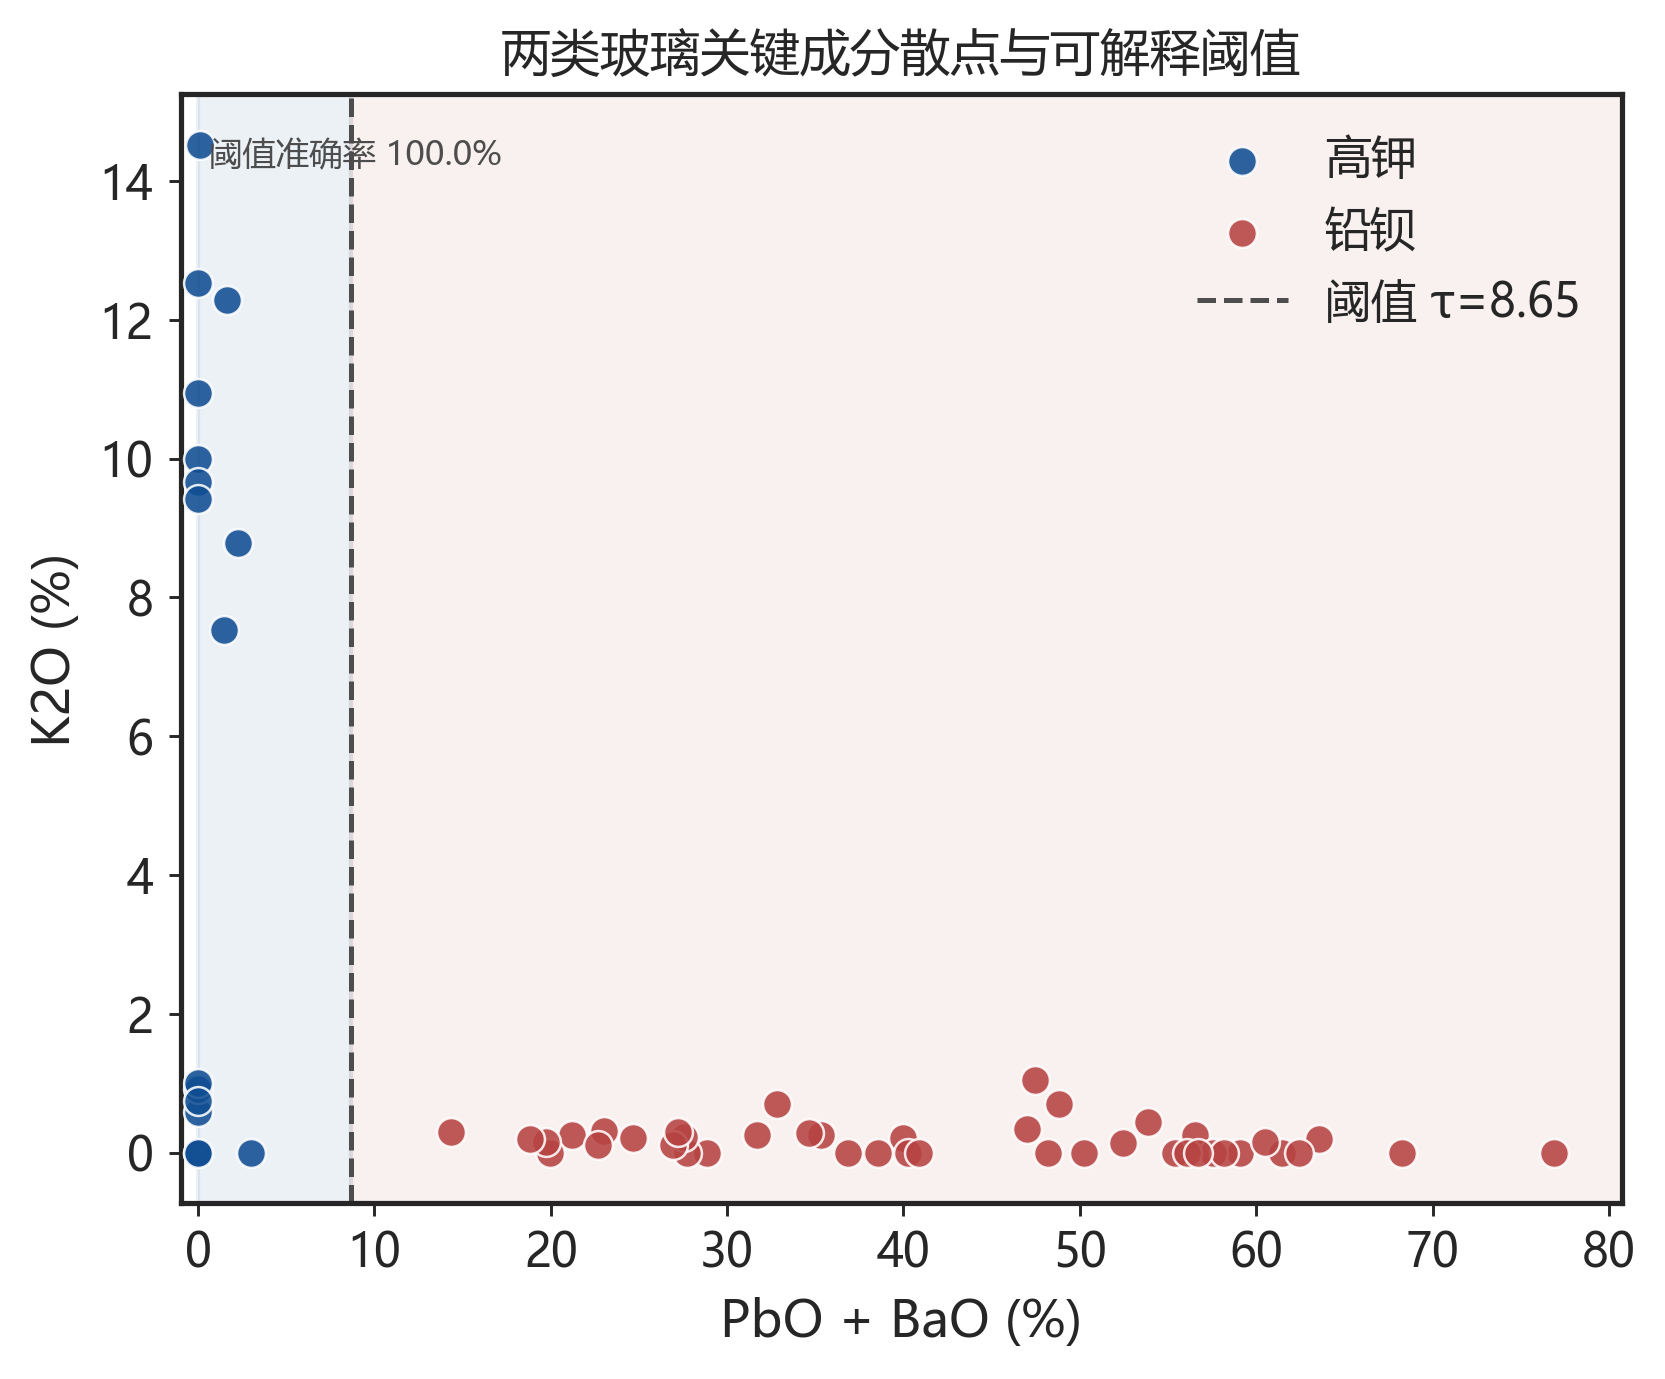
\includegraphics[width=0.72\textwidth]{fig2_3_scatter_rule.png}
\caption{两类玻璃在 $\mathrm{PbO}+\mathrm{BaO}$--$\mathrm{K_2O}$ 平面上的可解释分离（阈值仅在训练折内寻优）}
\label{fig:overview-rule}
\end{figure}

\textbf{问题一}属于分类变量关联 + 成分对比 + 逆向还原。先在文物层面做列联分析，再在采样点层面按“类型$\times$风化”分组比较 14 维成分，最后用组间风化系数把风化检测值映射回风化前状态。因无“风化前后成对”真值，还原结果应理解为\textbf{同类型平均意义下}的校正，而非个体埋藏史的精确反演。

\textbf{问题二}是有监督分类规律提取 + 无监督亚类发现。分类侧强调可解释规则（阈值/决策树）并与集成模型对照；亚类侧需处理成分数据的定和约束，故先对未检出做成分自适应小值替换并闭合，再引入 CLR 变换后聚类，并用轮廓系数与扰动 ARI 评价。

\textbf{问题三}是迁移预测：用已标注样本训练分类器，输出模型支持度及 bootstrap 区间，再在与问题二一致的 CLR 标准化空间按亚类质心归属；同时用 $\mathrm{PbO}+\mathrm{BaO}$ 阈值、输入扰动和适用域距离交叉核验。

\textbf{问题四}是成分关联及其组间差异。原始百分比相关会受定和约束和风化混杂影响，故以控制风化后的比例协调系数为主、Spearman 为对照，并用保持类型$\times$风化构成的分层标签置换直接检验两类关联矩阵之差。

% =========================================================
\section{模型假设与符号说明}
% =========================================================

\subsection{模型假设}
\begin{enumerate}[leftmargin=2em]
  \item 空白（未检出）成分按 $0$ 处理；累加和在 $[85,105]$ 内的采样点为有效数据。
  \item 表单 2 中“严重风化点”视为风化，“未风化点”视为无风化；其余采样点风化属性与表单 1 一致。
  \item 同一类型玻璃的风化过程具有统计上可迁移的平均规律，可用组间风化系数近似个体风化前成分；个体埋藏环境差异未观测，故预测为平均意义下的还原。
  \item 风化主要改变各氧化物相对比例，检测误差相对风化效应为小量。
  \item 亚类划分在给定类型内部进行，反映原料配比、工艺差异或风化程度差异，而非新的大类；小样本簇仅作候选亚型解释。
  \item CLR 变换前，各成分零值用该成分最小正检出值的一半替换；该规则随检测尺度自适应，且只由训练数据估计。
\end{enumerate}

\subsection{符号说明}
\begin{table}[H]
\centering
\caption{主要符号}
\begin{tabular}{cl}
\toprule
符号 & 含义 \\
\midrule
$x_{ij}$ & 第 $i$ 个采样点第 $j$ 种成分含量（\%） \\
$\mathcal{C}$ & 14 种氧化物指标集合 \\
$f_j^{(t)}$ & 类型 $t$ 下成分 $j$ 的风化系数 \\
$\hat{x}_{ij}^{(0)}$ & 风化前成分预测值 \\
$\mathrm{clr}(\cdot)$ & 中心对数比变换 \\
$V$ & Cramer's $V$ 关联系数 \\
ARI & 调整兰德指数 \\
FDR & 错误发现率（Benjamini--Hochberg） \\
\bottomrule
\end{tabular}
\end{table}

% =========================================================
\section{数据预处理}
% =========================================================

对表单 2 空白填 0，计算成分总和
\[
S_i=\sum_{j\in\mathcal{C}} x_{ij},
\]
保留 $S_i\in[85,105]$ 的样本。由“文物采样点”解析文物编号与特殊标记（部位1/2、未风化点、严重风化点），并与表单 1 合并。空白记 0 而非均值填补，是因为题面明确“空白表示未检出”；若用均值填补会虚构“已检出”信息。

\textbf{处理结果：}69 个采样点中有效 67 个；无效点为编号 15、17（总和越界）。后续描述性图件保留采样点信息；凡涉及显著性、泛化性能或类别间比较，均以文物编号分组或先合并为文物级单元，避免重复采样导致伪增样本量。

% =========================================================
\section{问题一：风化关系、成分规律与风化前预测}
% =========================================================

\subsection{风化与类型/纹饰/颜色的关联模型}

对因素 $A\in\{\text{类型},\text{纹饰},\text{颜色}\}$ 与表面风化做列联表，并报告 Cramer's $V$。考虑纹饰和颜色表中存在较多期望频数小于 5 的单元格，$2\times2$ 的“类型$\times$风化”采用 Fisher 精确检验，其余采用固定边际的 9999 次标签置换；渐近 $\chi^2$ 仅保留为统计量：
\[
\chi^2=\sum_{u,v}\frac{(O_{uv}-E_{uv})^2}{E_{uv}},\qquad
V=\sqrt{\frac{\chi^2}{n\cdot(\min(r,k)-1)}}.
\]

\begin{table}[H]
\centering
\caption{表面风化与各因素的关联检验}
\label{tab:p1-assoc}
\begin{tabular}{cccccc}
\toprule
因素 & $\chi^2$ & 自由度 & 稳健 $p$ 值 & Cramer's $V$ & 样本量 \\
\midrule
类型 & 6.880 & 1 & 0.0113（Fisher） & 0.344 & 58 \\
纹饰 & 4.957 & 2 & 0.1055（置换） & 0.292 & 58 \\
颜色 & 6.287 & 7 & 0.5860（置换） & 0.341 & 54 \\
\bottomrule
\end{tabular}
\end{table}

\begin{figure}[H]
\centering
\begin{subfigure}{0.48\textwidth}
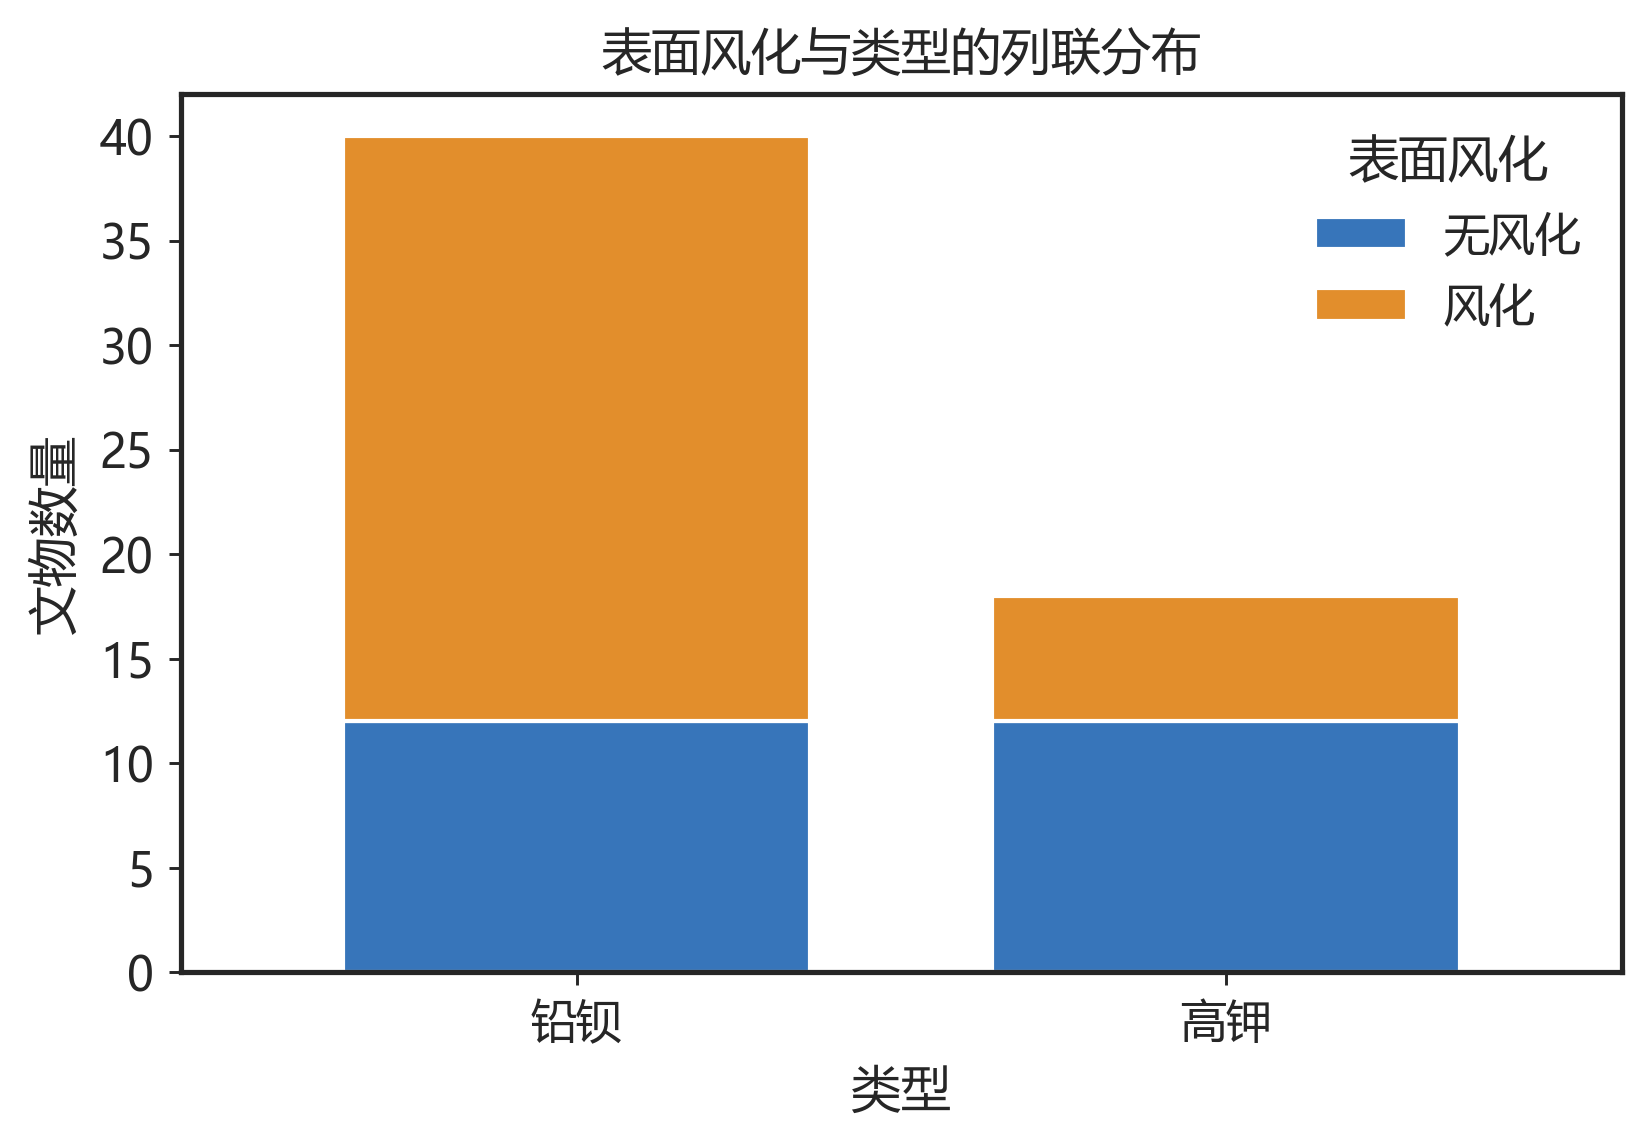
\includegraphics[width=\linewidth]{fig1_1_weather_类型.png}
\caption{与类型}
\end{subfigure}
\begin{subfigure}{0.48\textwidth}
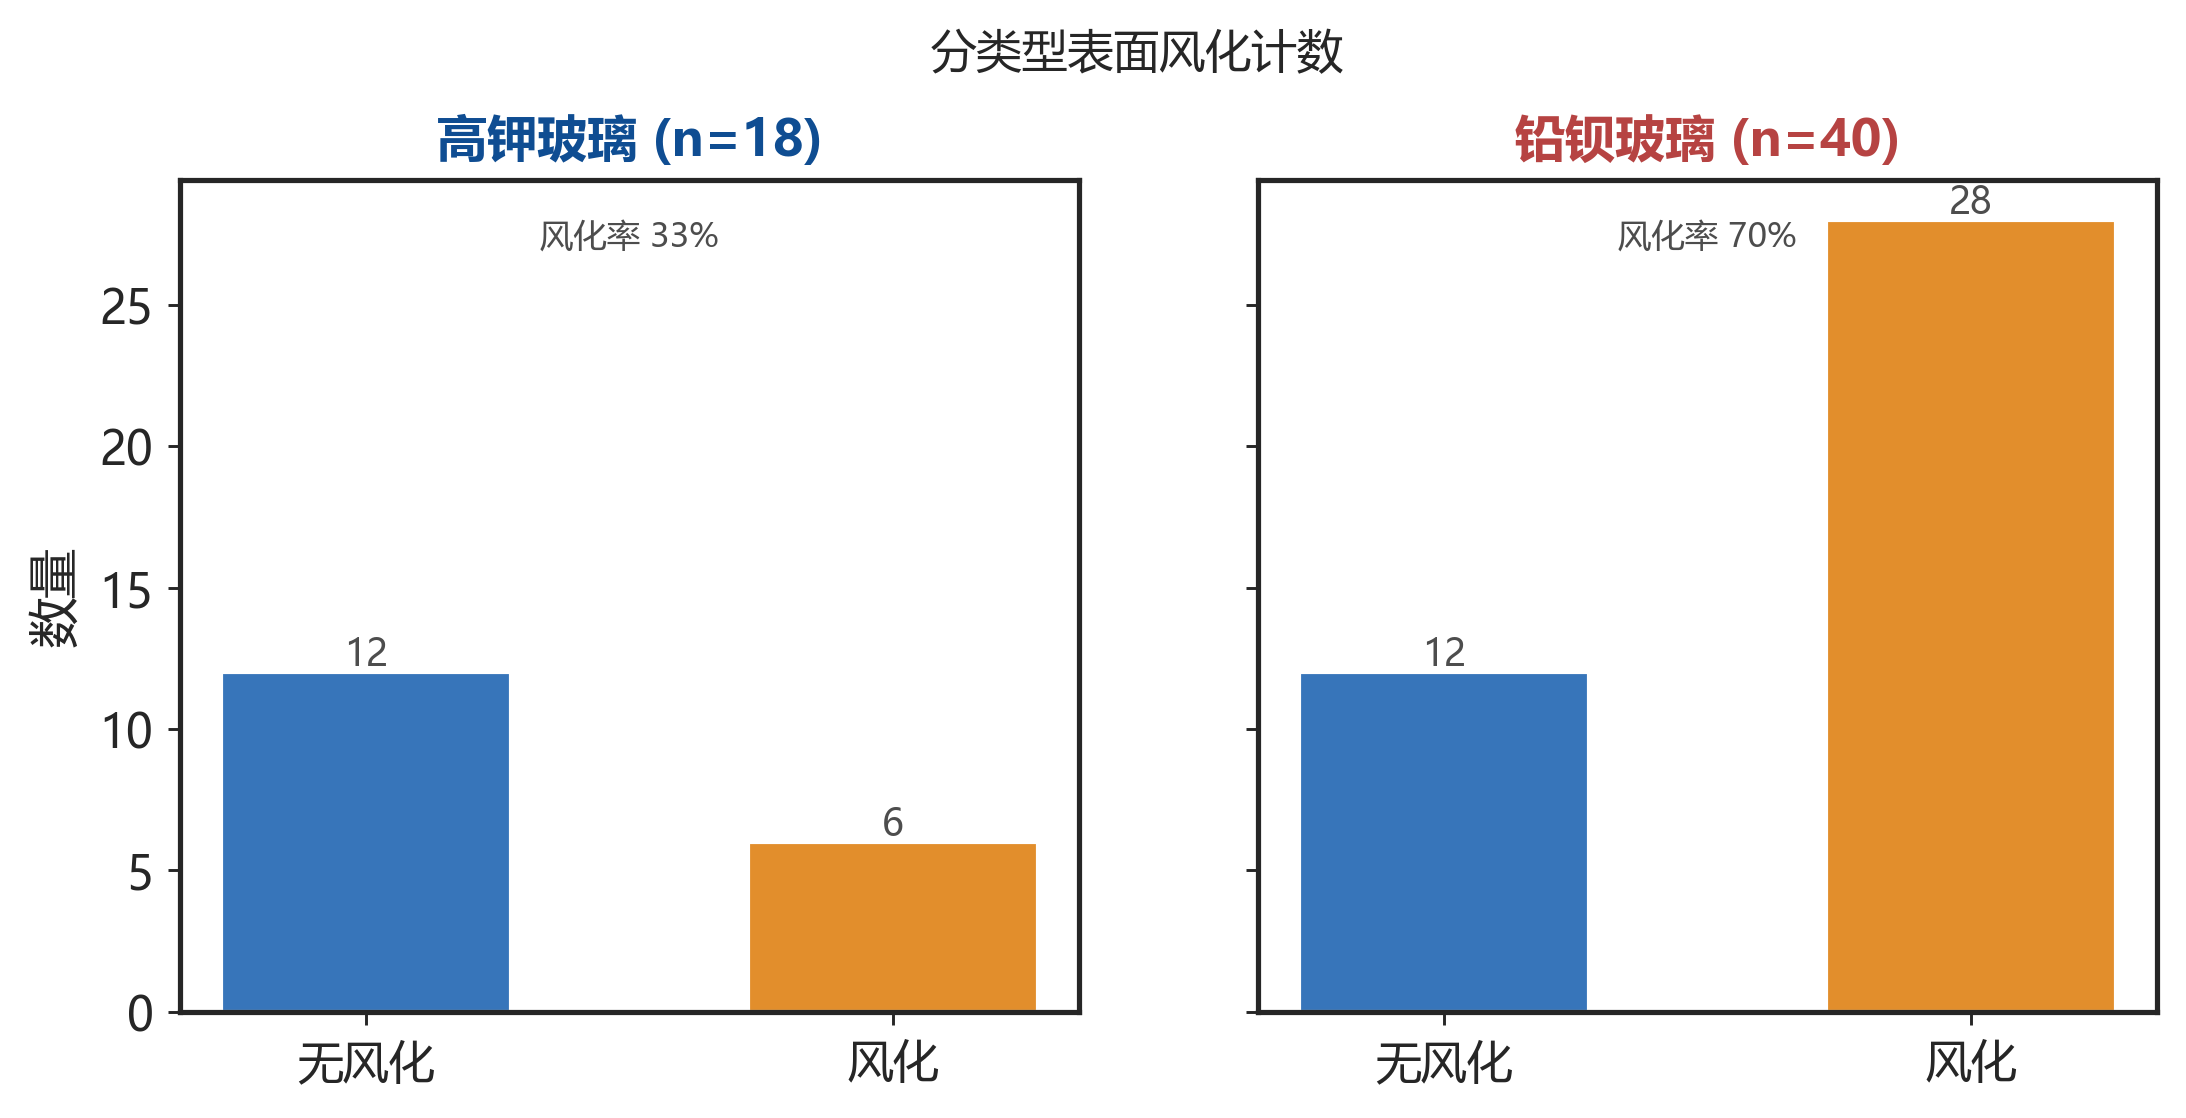
\includegraphics[width=\linewidth]{fig1_2_type_weather_count.png}
\caption{分类型计数}
\end{subfigure}
\caption{表面风化与玻璃类型的关系}
\label{fig:p1-type}
\end{figure}

\textbf{结论：}风化与\textbf{类型显著相关}（$p=0.0113$，中等效应）；稳健检验下纹饰（$p=0.1055$）与颜色（$p=0.5860$）均未达显著，不能再把纹饰表述为“边缘显著”。铅钡玻璃风化比例更高，但该结果是关联而非材料脆弱性的因果证明。

\subsection{分类型的有无风化成分统计规律}

对类型 $t\in\{\text{高钾},\text{铅钡}\}$，先将同一文物、同一风化状态的重复采样取均值。编号49、50同时含风化与未风化点，为避免在独立样本检验中重复计权，将其留作风化位移估计但不进入 Mann--Whitney $U$ 检验；其余文物各贡献一个独立单元。对每一类型的 14 次检验分别采用 Benjamini--Hochberg 程序控制 FDR。用于描述的\textbf{风化系数}定义为
\[
f_j^{(t)}=\frac{\bar{x}_{j,w}^{(t)}}{\bar{x}_{j,u}^{(t)}},
\]
并用 bootstrap（$B=1000$）估计其 $95\%$ 置信区间。若某成分在两组中检出率均过低、系数极端（$>8$ 或 $\le0$）或置信区间过宽，则标记为\textbf{不稳定}，预测阶段取 $f_j^{(t)}=1$（不校正），避免稀有检出（如 $\mathrm{SO_2}$）拉爆系数。

\begin{figure}[H]
\centering
\begin{subfigure}{0.48\textwidth}
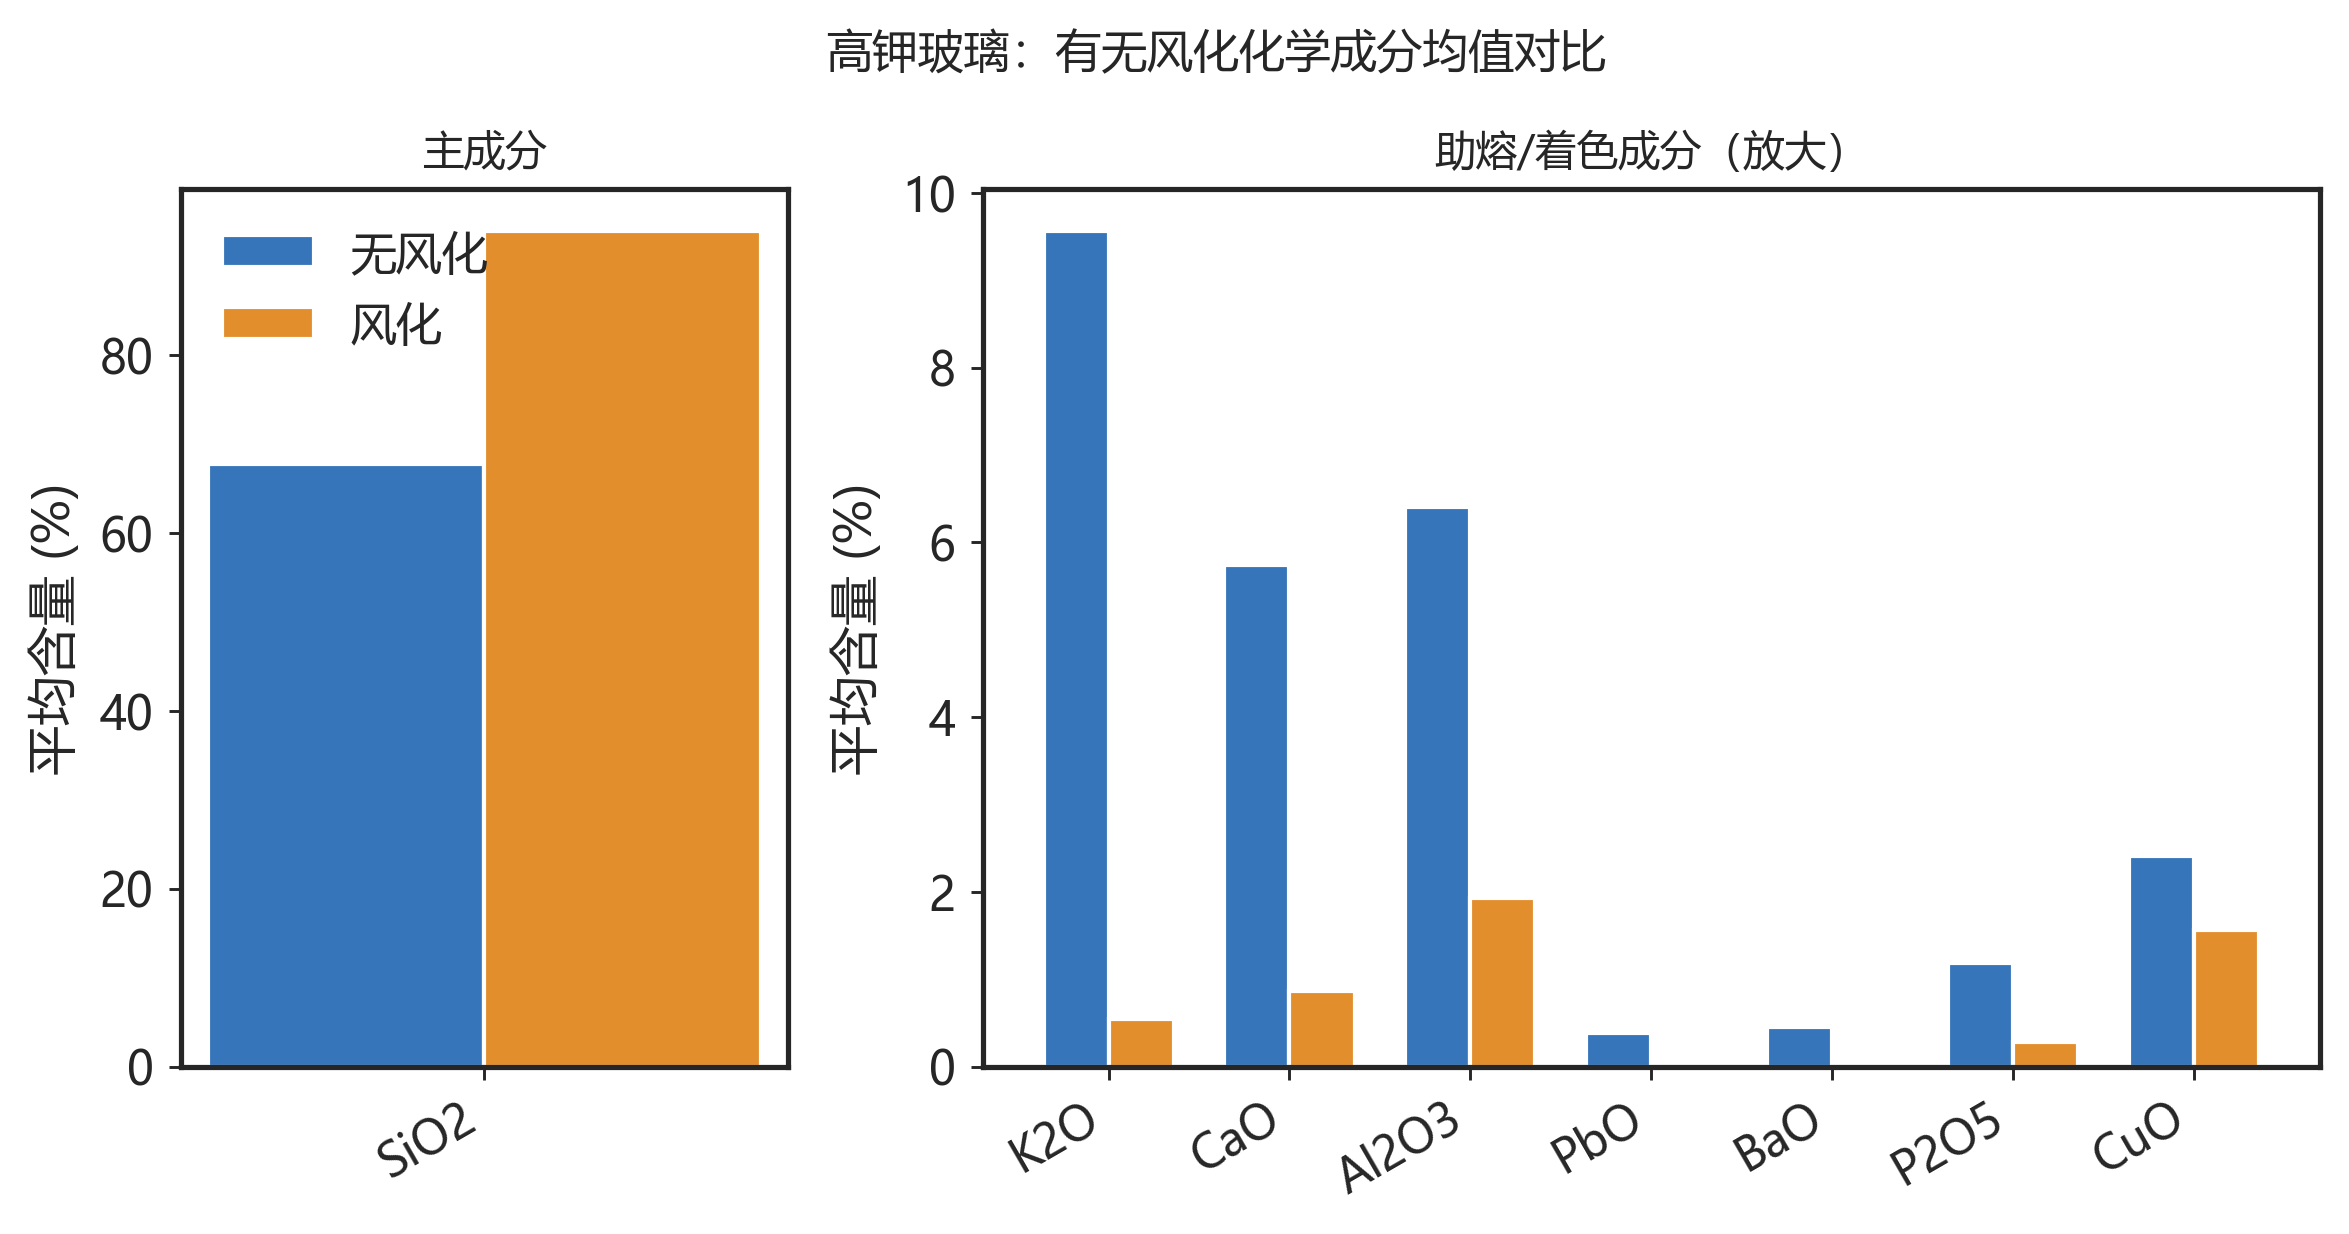
\includegraphics[width=\linewidth]{fig1_3_mean_高钾.png}
\caption{高钾}
\end{subfigure}
\begin{subfigure}{0.48\textwidth}
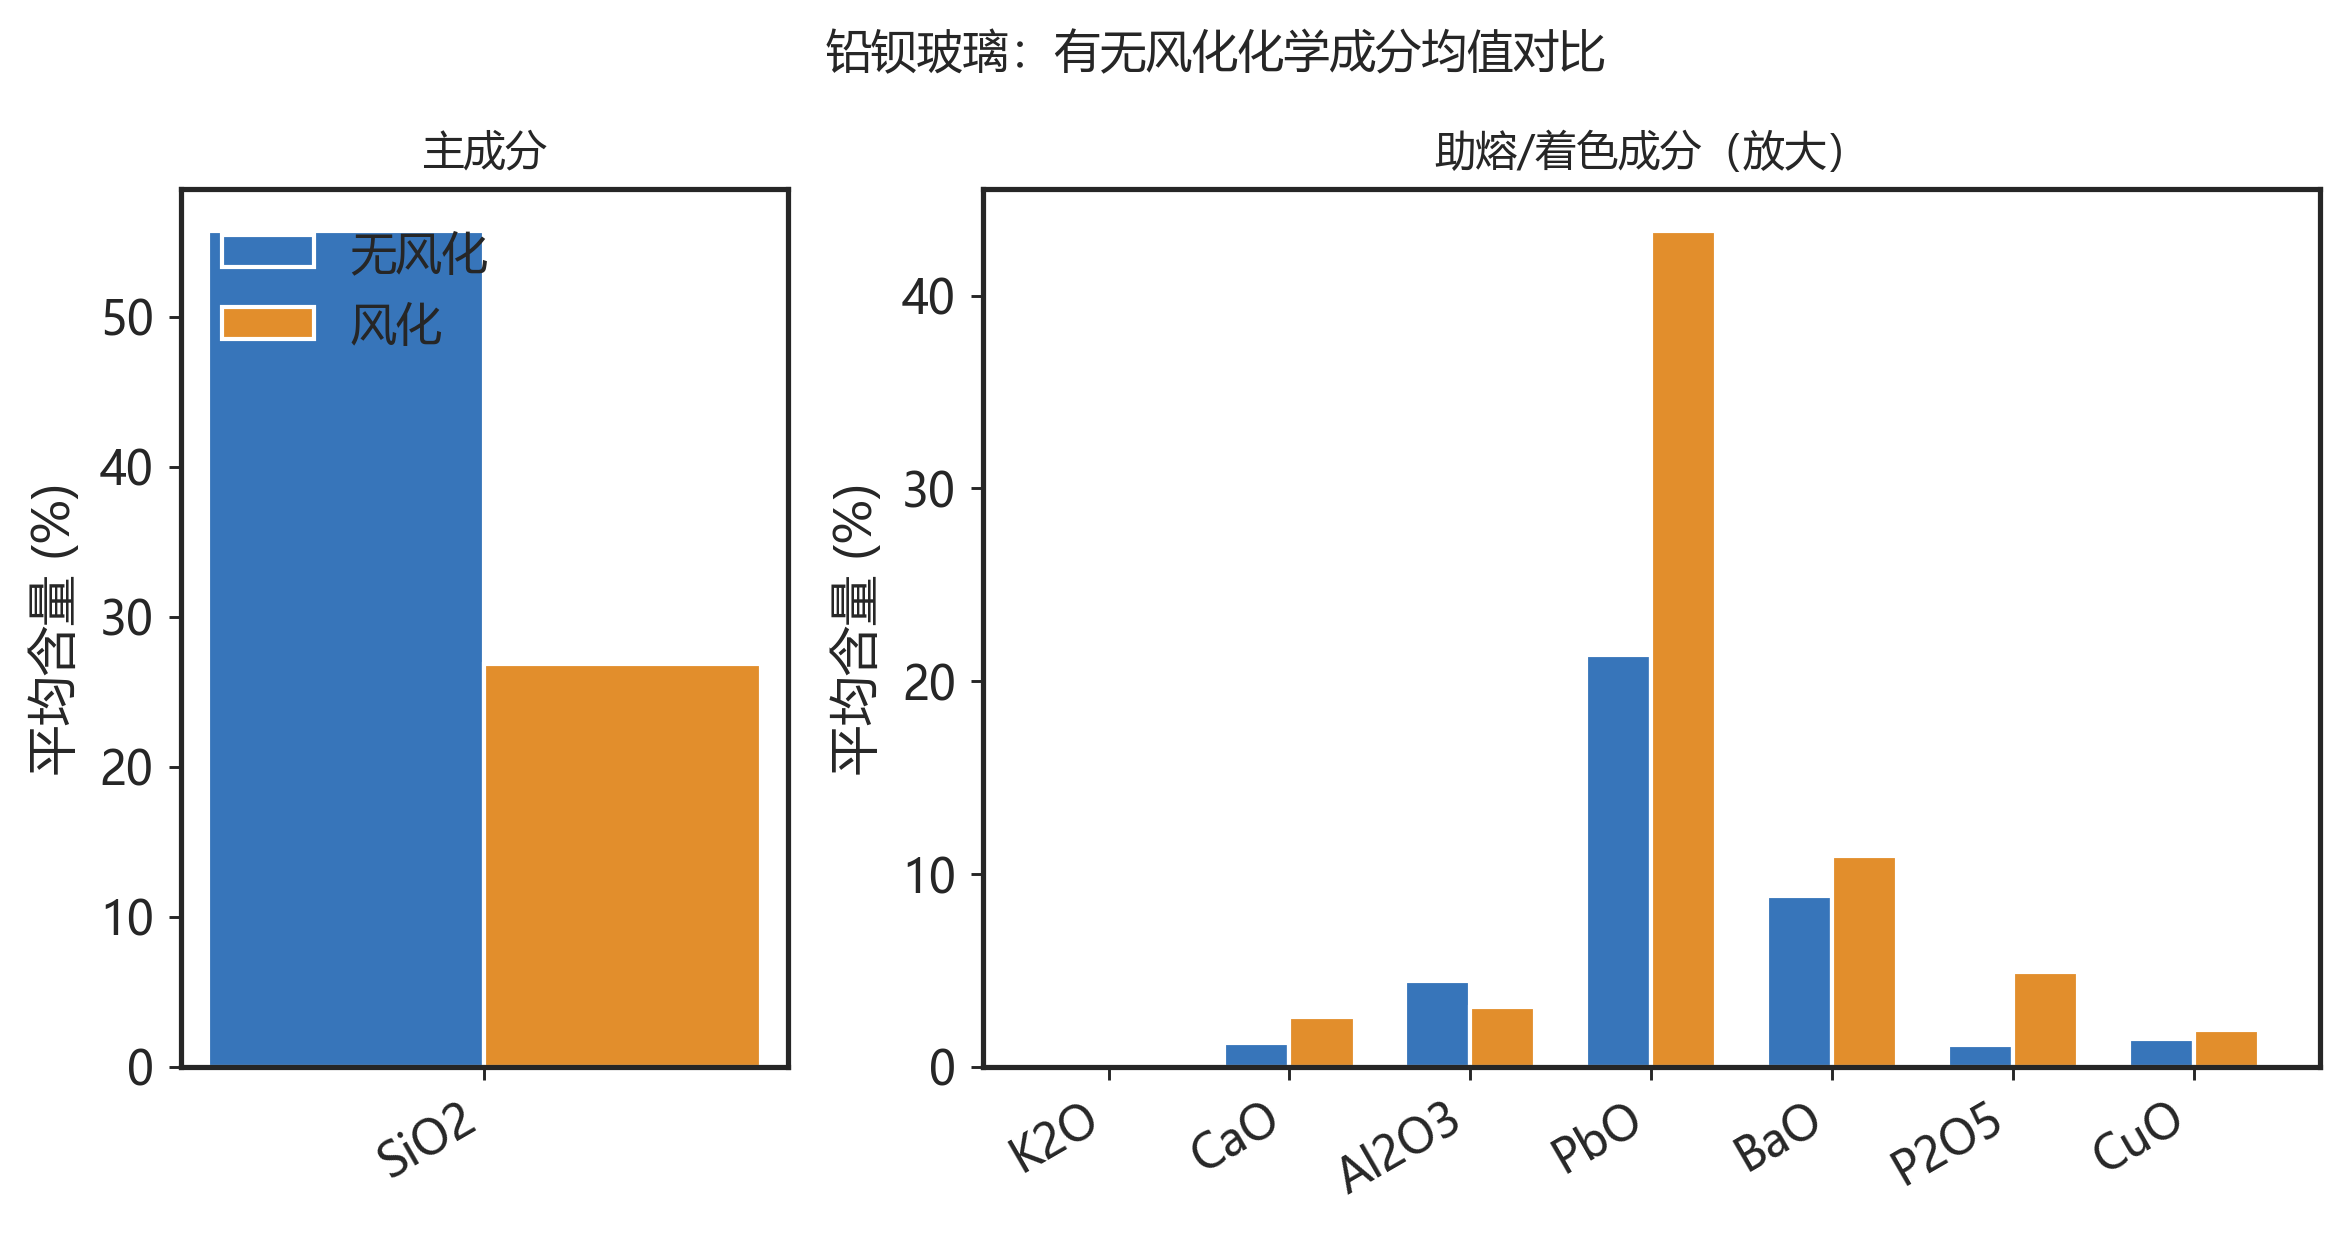
\includegraphics[width=\linewidth]{fig1_3_mean_铅钡.png}
\caption{铅钡}
\end{subfigure}
\caption{两类玻璃有无风化主要成分均值对比（右面板放大助熔/着色成分）}
\label{fig:p1-mean}
\end{figure}

\begin{figure}[H]
\centering
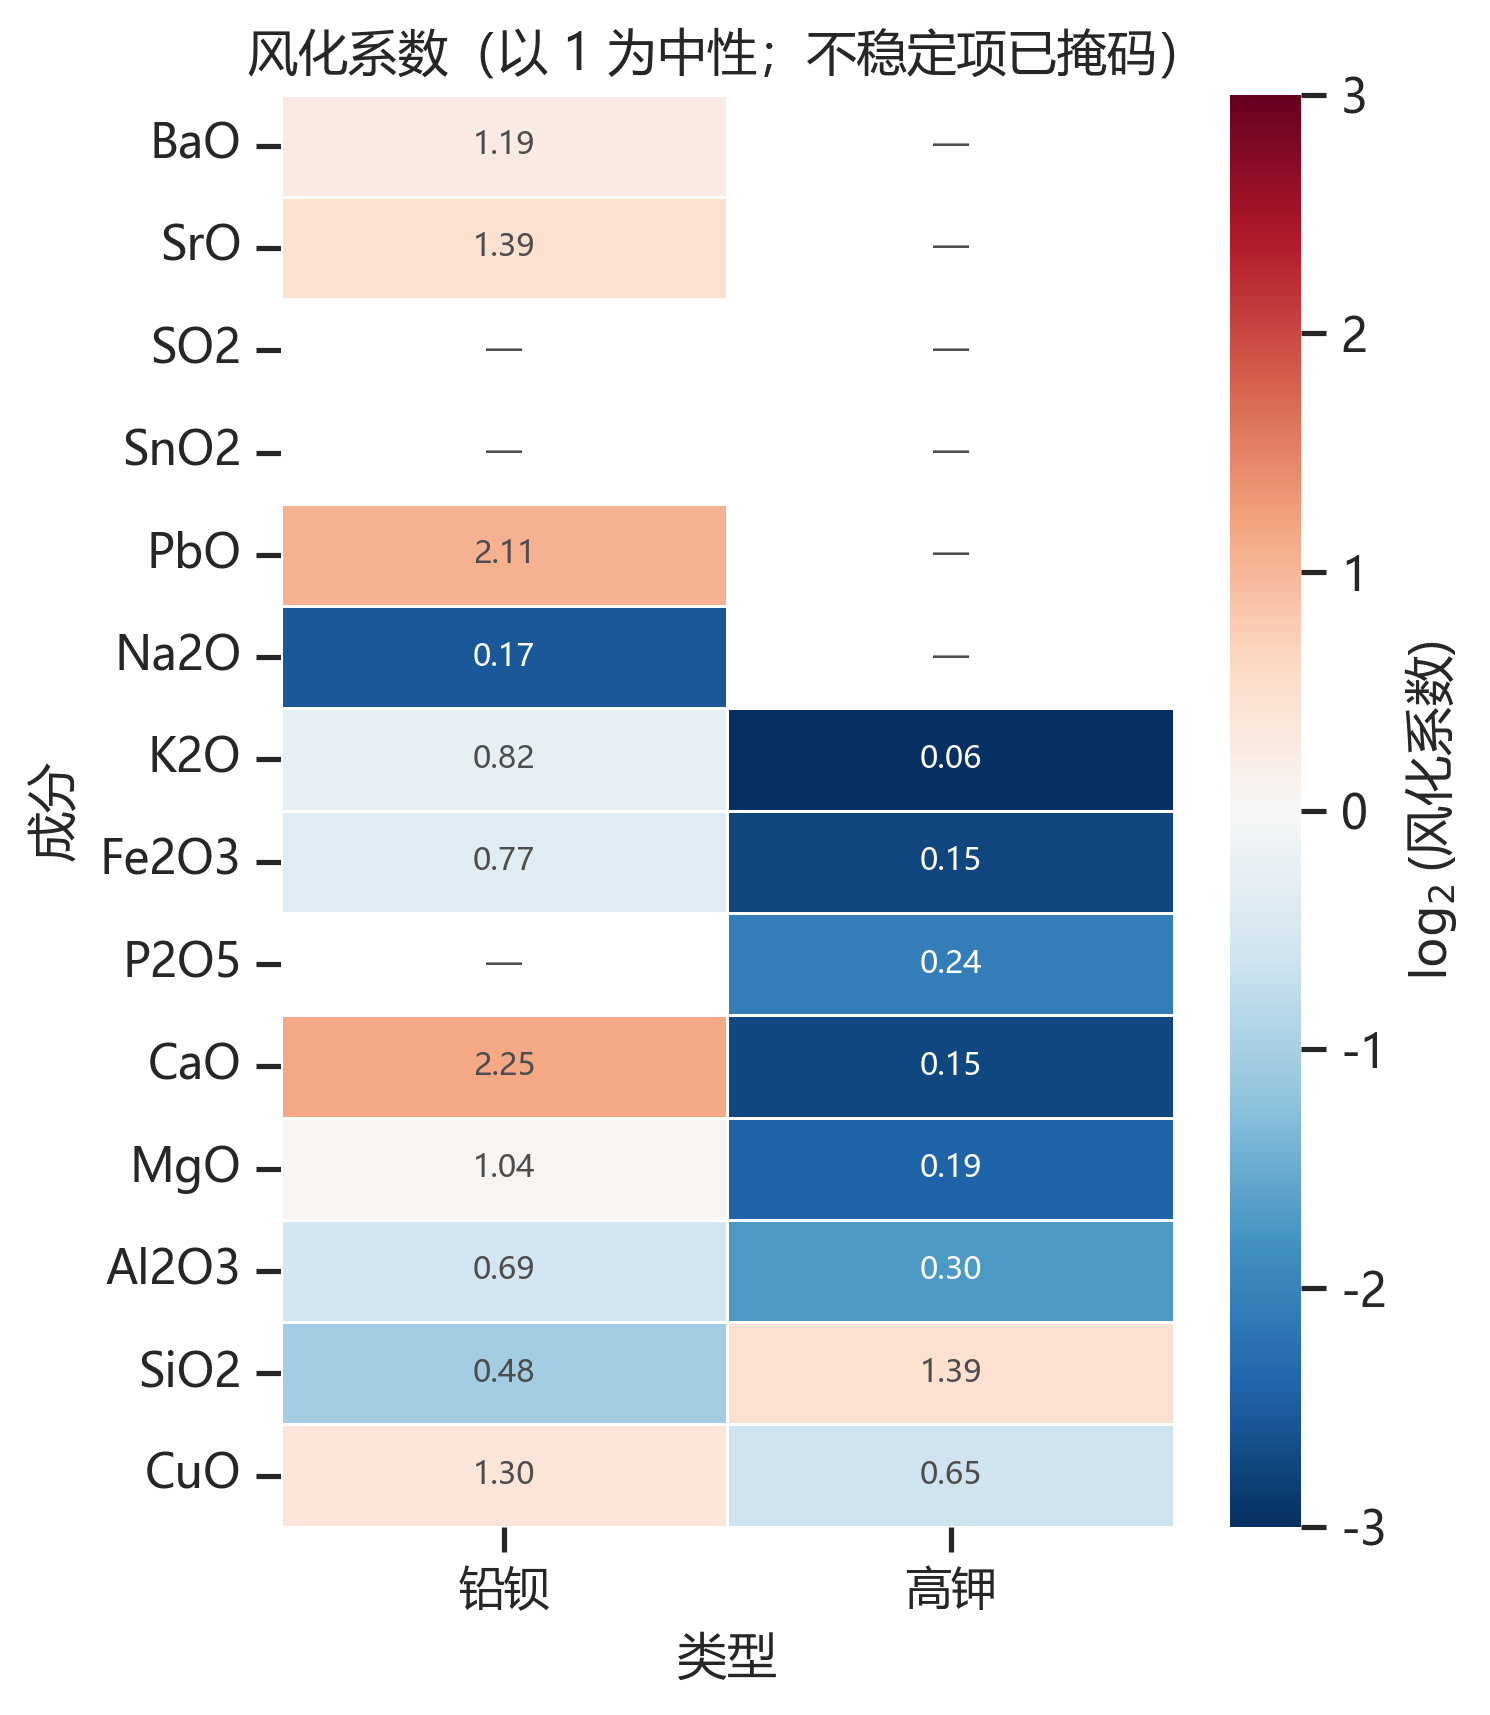
\includegraphics[width=0.52\textwidth]{fig1_4_weather_factor.png}
\caption{风化系数热图（色标为 $\log_2 f$，以 $f=1$ 为中性；不稳定项掩码为“---”）}
\label{fig:p1-factor}
\end{figure}

\begin{table}[H]
\centering
\caption{FDR 显著变化成分摘要（$\mathrm{FDR}<0.05$）}
\label{tab:p1-sig}
\small
\begin{tabular}{llcccc}
\toprule
类型 & 成分 & 无风化均值 & 风化均值 & 风化系数 & 变化方向 \\
\midrule
高钾 & $\mathrm{SiO_2}$ & 67.77 & 93.96 & 1.39 & 显著升高 \\
高钾 & $\mathrm{K_2O}$ & 9.57 & 0.54 & 0.06 & 显著流失 \\
高钾 & $\mathrm{CaO}$ & 5.73 & 0.87 & 0.15 & 显著流失 \\
高钾 & $\mathrm{MgO}$ & 1.05 & 0.20 & 0.19 & 显著流失 \\
高钾 & $\mathrm{Al_2O_3}$ & 6.41 & 1.93 & 0.30 & 显著流失 \\
高钾 & $\mathrm{Fe_2O_3}$ & 1.79 & 0.27 & 0.15 & 显著流失 \\
铅钡 & $\mathrm{SiO_2}$ & 56.35 & 27.22 & 0.48 & 显著下降 \\
铅钡 & $\mathrm{CaO}$ & 1.07 & 2.42 & 2.25 & 显著升高 \\
铅钡 & $\mathrm{PbO}$ & 20.78 & 43.82 & 2.11 & 显著富集 \\
铅钡 & $\mathrm{P_2O_5}$ & 0.67 & 4.50 & 6.73 & 显著富集 \\
\bottomrule
\end{tabular}
\end{table}

\textbf{规律解读（化学含义）：}
\begin{itemize}[leftmargin=2em]
  \item \textbf{高钾玻璃：}风化使碱金属与碱土助熔剂大量淋失，$\mathrm{SiO_2}$ 相对残留升高，表面呈现“高硅贫钾”。这与钾玻璃网络中可迁移阳离子易被地下水带走的机制一致。
  \item \textbf{铅钡玻璃：}硅酸盐网络破坏后，$\mathrm{PbO}$、$\mathrm{P_2O_5}$ 等在风化层相对富集，$\mathrm{SiO_2}$ 反而下降。路径与高钾相反，说明两类玻璃不能共用同一套风化校正公式，必须\textbf{分类型}估计风化系数。
\end{itemize}

\subsection{风化前化学成分预测模型}

逐成分相除后再闭合并不遵守 Aitchison 几何，且零值会使比例爆炸。本文改在 CLR 空间估计类型 $t$ 的平均风化位移
\[
\bm{\delta}^{(t)}
=\lambda_t\!\left(\overline{\mathrm{clr}(\bm{x})}_{w,t}
-\overline{\mathrm{clr}(\bm{x})}_{u,t}\right),\qquad
\lambda_t=\frac{n_{\mathrm{eff}}}{n_{\mathrm{eff}}+4},
\]
其中 $\lambda_t$ 将小样本估计收缩到“无风化效应”。对风化点的还原为
\[
\hat{\bm{x}}_i^{(0)}
=\mathcal{C}_{S_i}\!\left[
\exp\!\left(\mathrm{clr}(\bm{x}_i)-\bm{\delta}^{(t)}\right)\right],
\]
$\mathcal{C}_{S_i}$ 表示闭合到原检测总和 $S_i$。描述性风化系数仍用于解释升降方向，但不再直接充当逆变换。

\begin{figure}[H]
\centering
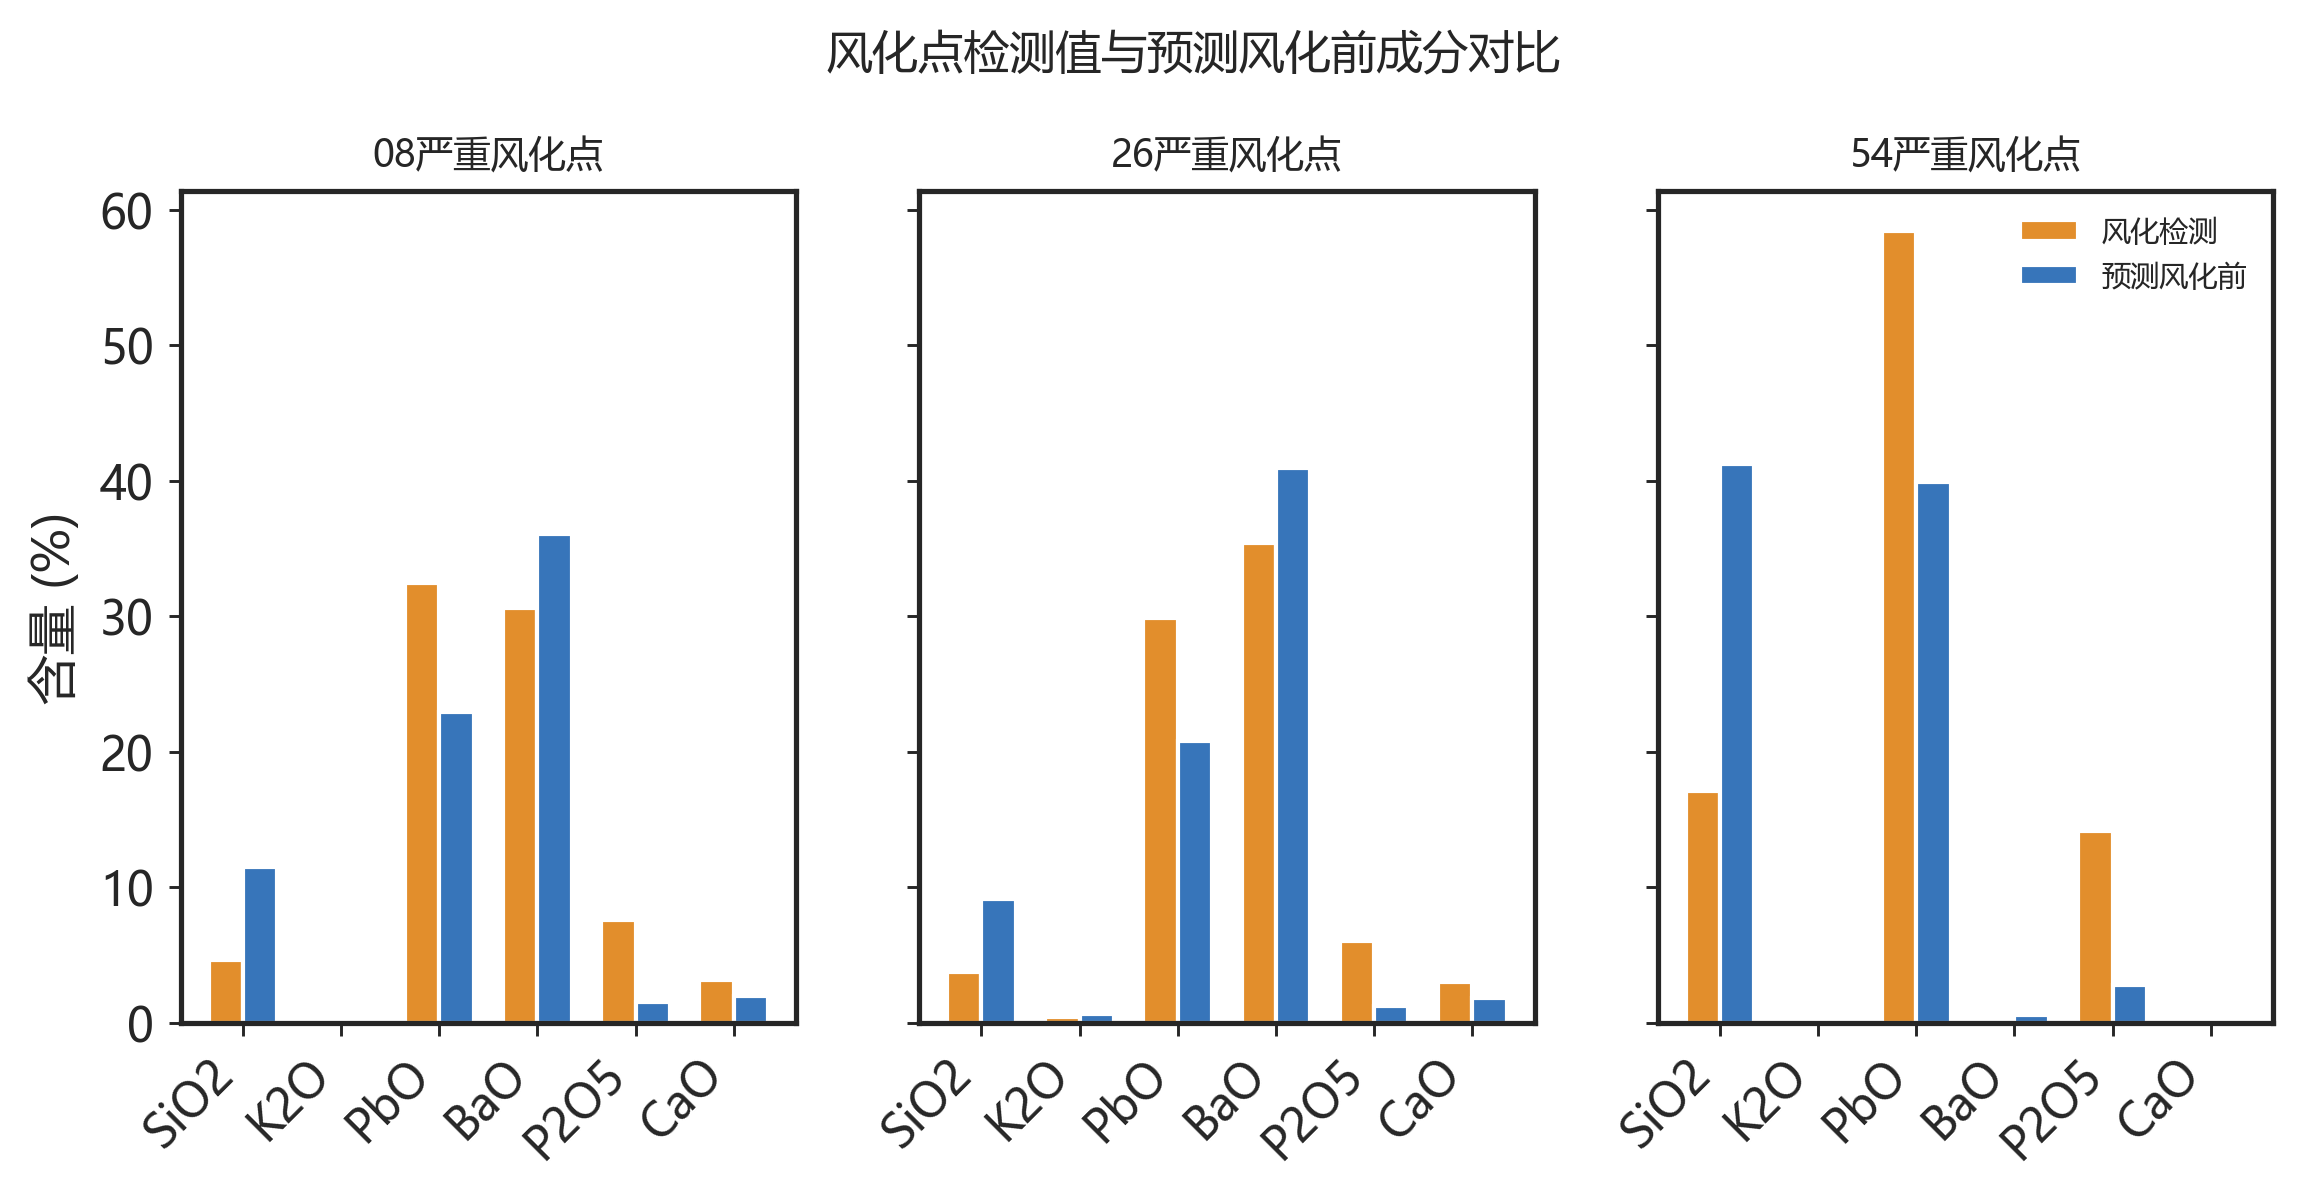
\includegraphics[width=0.95\textwidth]{fig1_5_preweather_pred.png}
\caption{典型风化点：检测值与预测风化前成分对比}
\label{fig:p1-pred}
\end{figure}

\begin{table}[H]
\centering
\caption{部分风化点风化前预测结果（\%，节选）}
\label{tab:p1-pred}
\small
\begin{tabular}{llcccccc}
\toprule
采样点 & 类型 & $\mathrm{SiO_2}$ & $\mathrm{K_2O}$ & $\mathrm{CaO}$ & $\mathrm{PbO}$ & $\mathrm{BaO}$ & $\mathrm{P_2O_5}$ \\
\midrule
02 & 铅钡 & 62.28 & 1.22 & 1.00 & 23.06 & 0.40 & 0.51 \\
07 & 高钾 & 80.65 & 1.68 & 3.49 & 0.12 & 0.67 & 1.40 \\
09 & 高钾 & 84.21 & 3.41 & 2.06 & 0.13 & 0.68 & 0.82 \\
08严重风化点 & 铅钡 & 11.52 & 0.09 & 1.98 & 22.96 & 36.06 & 1.56 \\
\bottomrule
\end{tabular}
\end{table}

完整 32 个风化点预测见支撑材料 \texttt{p1\_predict\_preweather.csv}。需强调：该方法给出的是“若该点遵循同类型平均风化轨迹，其风化前成分应大致如何”，而非对单件文物埋藏史的唯一真值。

% =========================================================
\section{问题二：分类规律与亚类划分}
% =========================================================

\subsection{高钾/铅钡分类规律}

以 14 维成分为特征，类型为标签。采用：
\begin{enumerate}[leftmargin=2em]
  \item 深度受限决策树（可解释规则）；
  \item 原始成分随机森林与 CLR--Logistic 的等权集成（降低单一模型偏差）；
  \item 单指标阈值规则：$\mathrm{PbO}+\mathrm{BaO}\ge \tau$。
\end{enumerate}

关键改进是验证单位。表单2含同一文物的多采样点，普通逐点留一会把同源信息同时放入训练集和验证集。本文使用 Leave-One-Group-Out，以文物编号为组；每一折的零值替换、标准化、模型拟合及阈值寻优均只使用训练文物。决策树（分组留一准确率 $98.3\%$）给出核心规则：
\[
\begin{cases}
\mathrm{PbO}\le 5.46 &\Rightarrow \text{高钾},\\
\mathrm{PbO}>5.46 &\Rightarrow \text{铅钡}.
\end{cases}
\]
随机森林重要性排序前五为 $\mathrm{BaO},\mathrm{PbO},\mathrm{SrO},\mathrm{SiO_2},\mathrm{K_2O}$。最终全训练集阈值为 $\tau^*=8.655$；更重要的是，阈值在每一验证折内重新选择后仍取得 $100\%$ 的分组留一准确率，集成模型也为 $100\%$（Brier 分数 $0.0096$）。这说明两类在该数据中分离很强，但由于样本少，$100\%$ 仅代表内部验证，不能外推为真实考古样本的无误差率。

\begin{figure}[H]
\centering
\begin{subfigure}{0.48\textwidth}
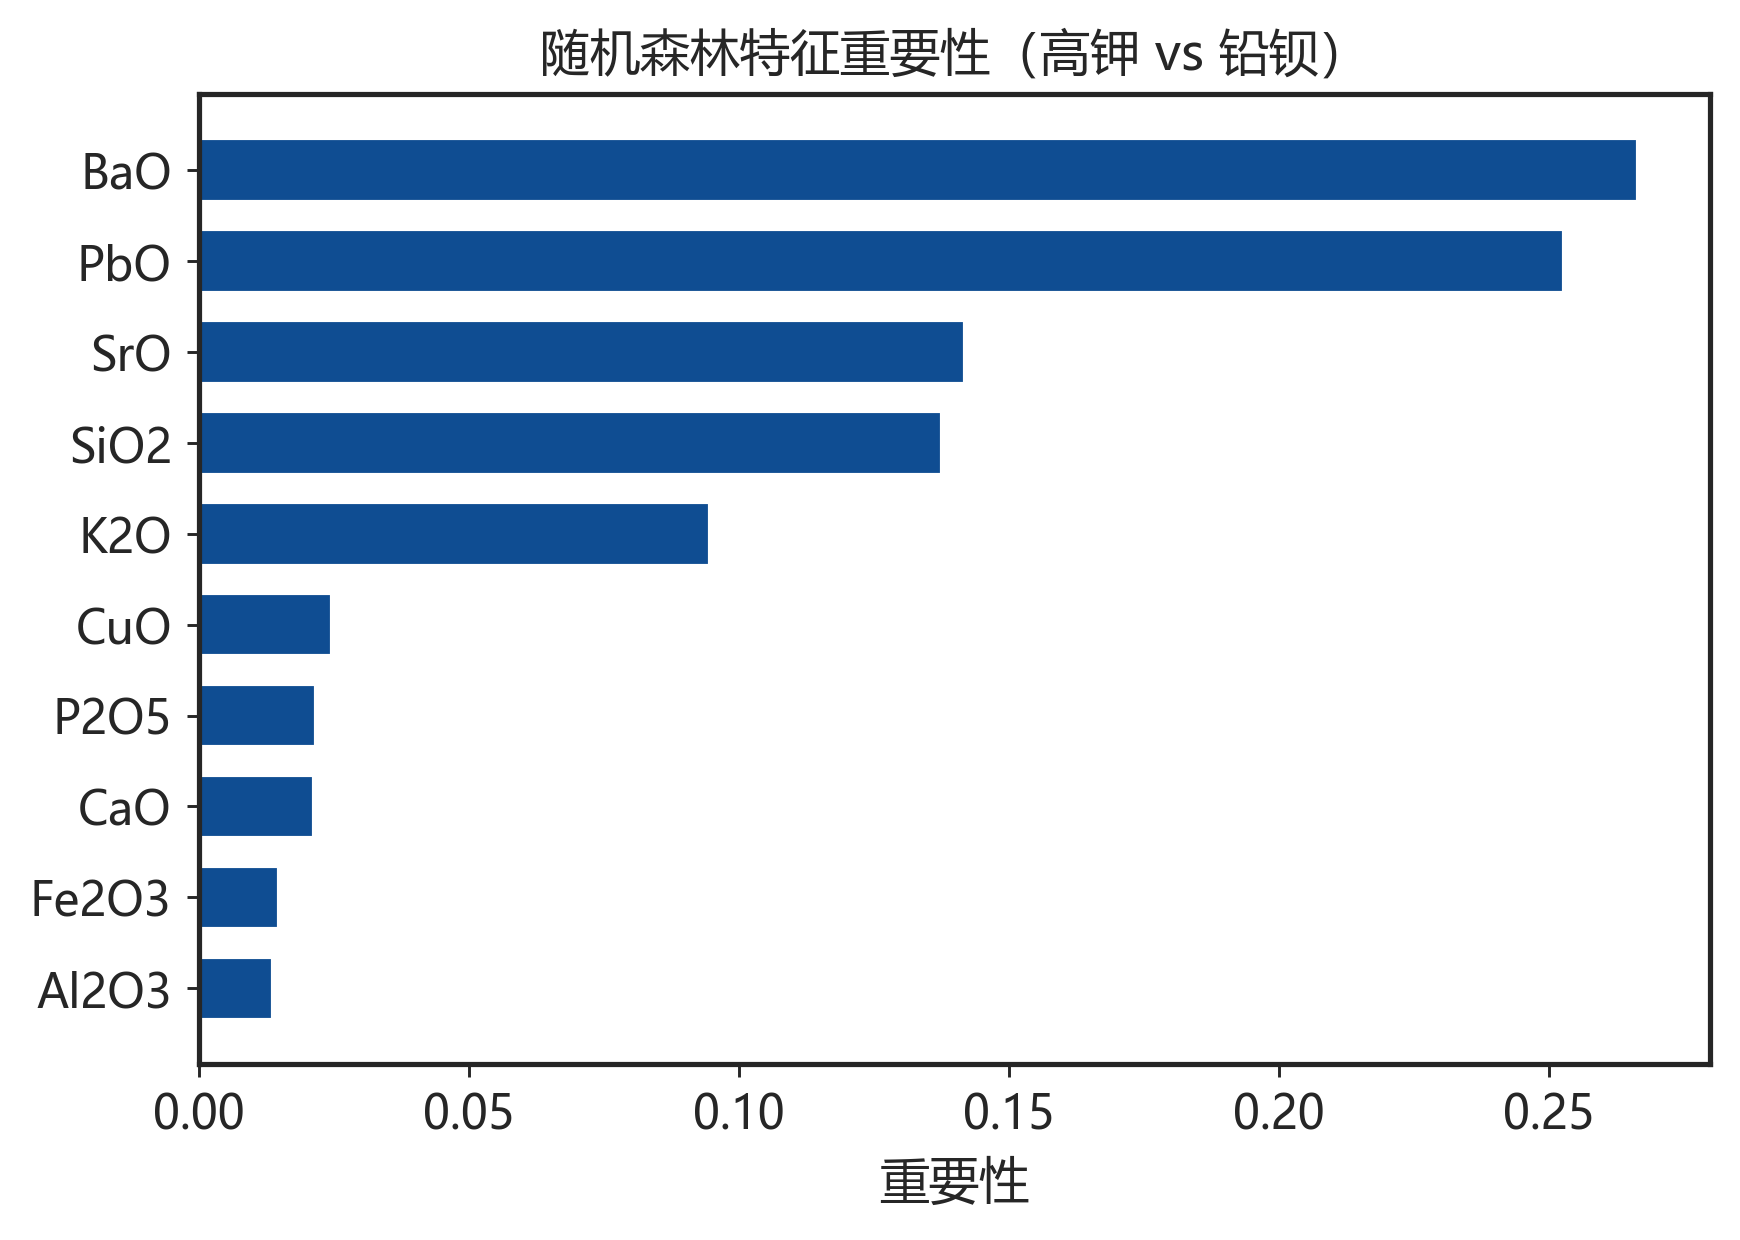
\includegraphics[width=\linewidth]{fig2_1_feature_importance.png}
\caption{特征重要性}
\end{subfigure}
\begin{subfigure}{0.48\textwidth}
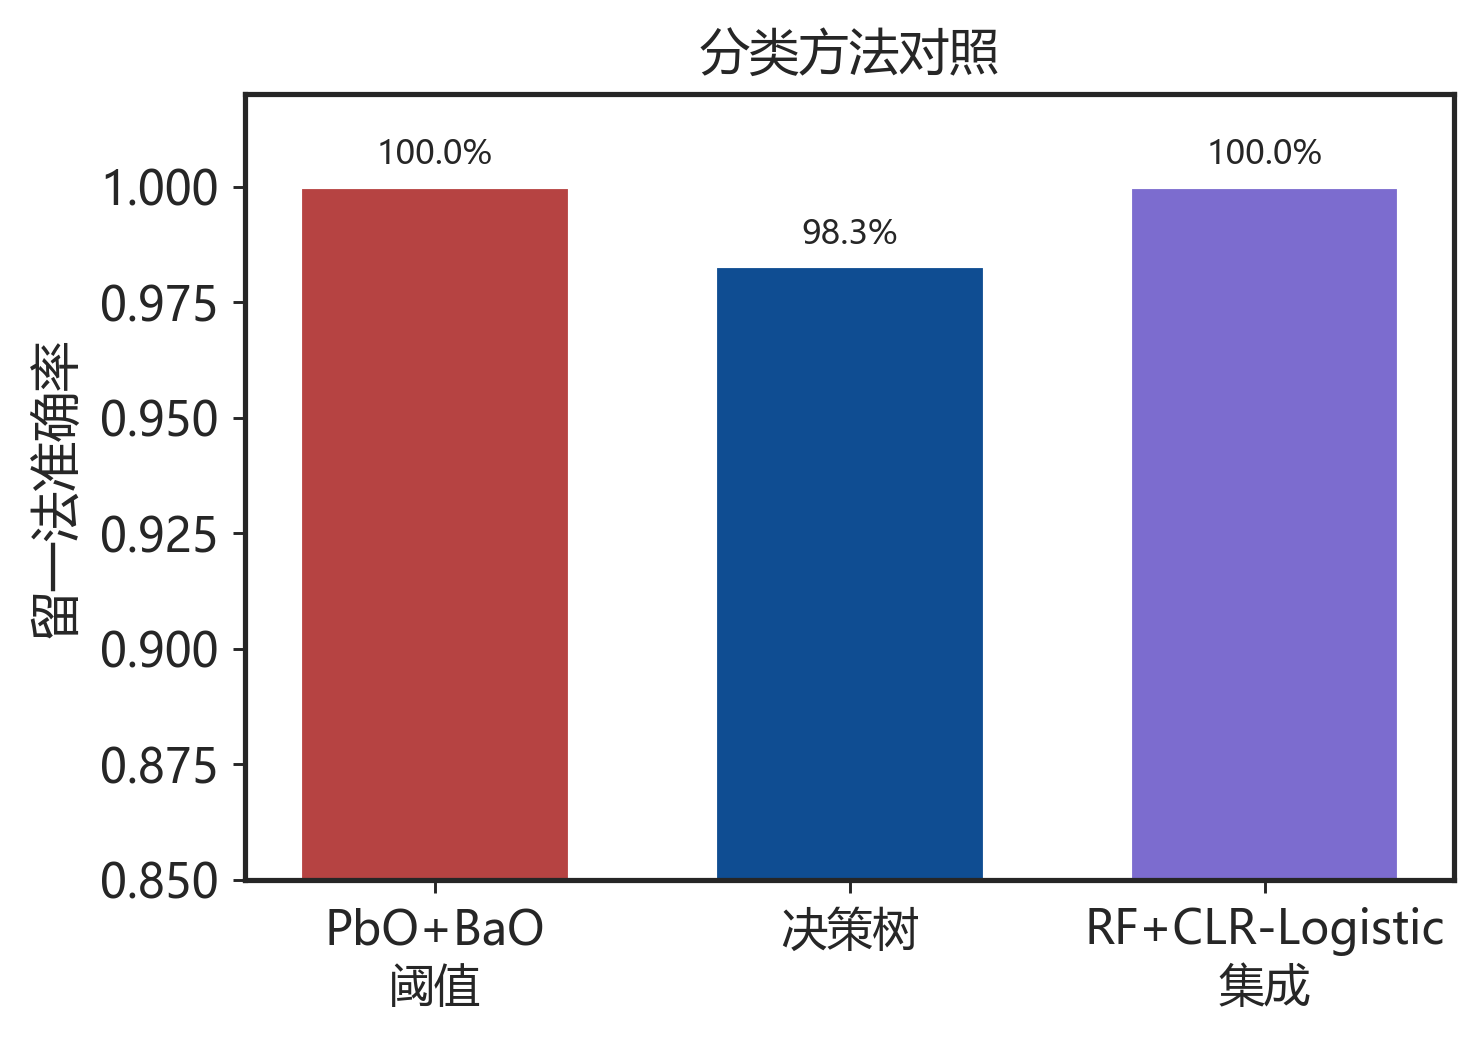
\includegraphics[width=\linewidth]{fig2_9_method_compare.png}
\caption{方法对照}
\end{subfigure}
\caption{分类规律：重要性与方法准确率对照}
\label{fig:p2-rule}
\end{figure}

\begin{figure}[H]
\centering
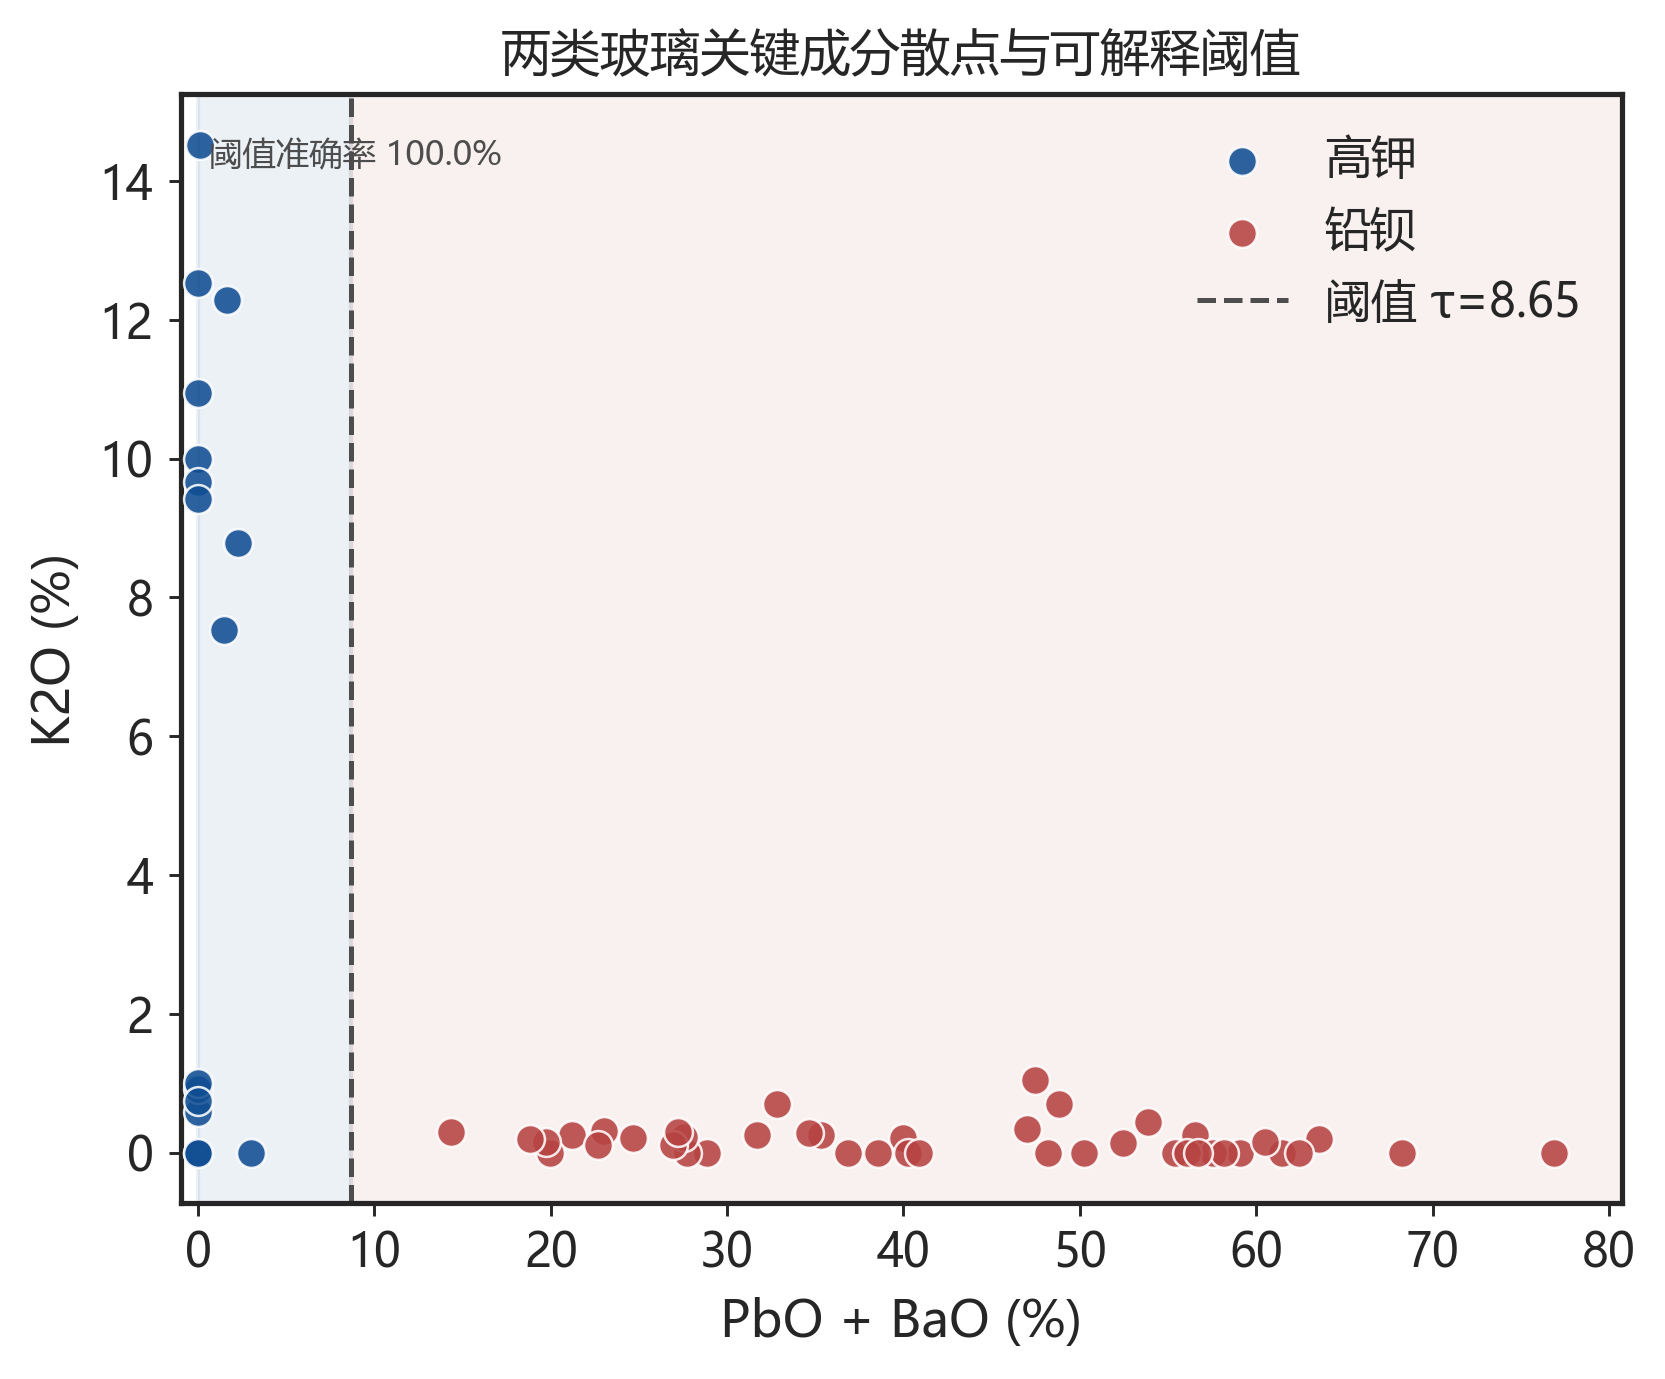
\includegraphics[width=0.72\textwidth]{fig2_3_scatter_rule.png}
\caption{$\mathrm{PbO}+\mathrm{BaO}$ 阈值判别（阴影为分区；标注了落在阈值右侧的高钾例外点）}
\label{fig:p2-scatter}
\end{figure}

图~\ref{fig:p2-scatter} 显示两类在 $\mathrm{PbO}+\mathrm{BaO}$ 轴上近乎线性可分。阈值图用于解释“铅钡助熔剂”这一判别规律；正式未知样本鉴别仍由集成支持度、阈值一致性和适用域三项共同决定。

作为对照，标准化成分的 PCA 前两维累计方差约 $46.5\%$（PC1 主载荷为 $\mathrm{BaO},\mathrm{SiO_2},\mathrm{PbO}$），只能作整体可分性示意，\textbf{不宜单独作为分类依据}。

\subsection{亚类划分方法}

成分数据满足定和约束，直接欧氏聚类易产生假结构。先将未检出替换为 $\varepsilon$，再对选定成分向量 $\bm{x}$ 做 CLR：
\[
\mathrm{clr}(\bm{x})=\left(\ln\frac{x_1}{g(\bm{x})},\ldots,\ln\frac{x_p}{g(\bm{x})}\right),
\quad g(\bm{x})=\big(\prod_{j=1}^p x_j\big)^{1/p}.
\]
为避免把“风化程度”误分成“工艺亚类”，先用问题一的分类型 CLR 位移校正所有风化点，再将同一文物多点取均值。在校正后的文物级 CLR 标准化空间使用 Ward 层次聚类；考虑高钾仅 16 件，最小簇规模设为 2、搜索 $k=2,3$，铅钡最小簇规模设为 3、搜索 $k=2,3,4$。完全按轮廓系数选型，不再人为偏好 $k=3$；亚类编号按 $\mathrm{SiO_2}$ 均值从高到低排列。

\textbf{结果：}高钾取 $k=2$（$14/2$，轮廓系数 $0.341$），铅钡取 $k=4$（$3/5/16/16$，轮廓系数 $0.321$）。与旧流程强行偏好 $k=3$ 相比，新结果更忠实反映数据：高钾的第二组仅 2 件，属于离群型候选组；铅钡存在中等偏弱的四组结构，其中 $n=3,5$ 的小组仍不可作确定工艺类型。

\begin{figure}[H]
\centering
\begin{subfigure}{0.48\textwidth}
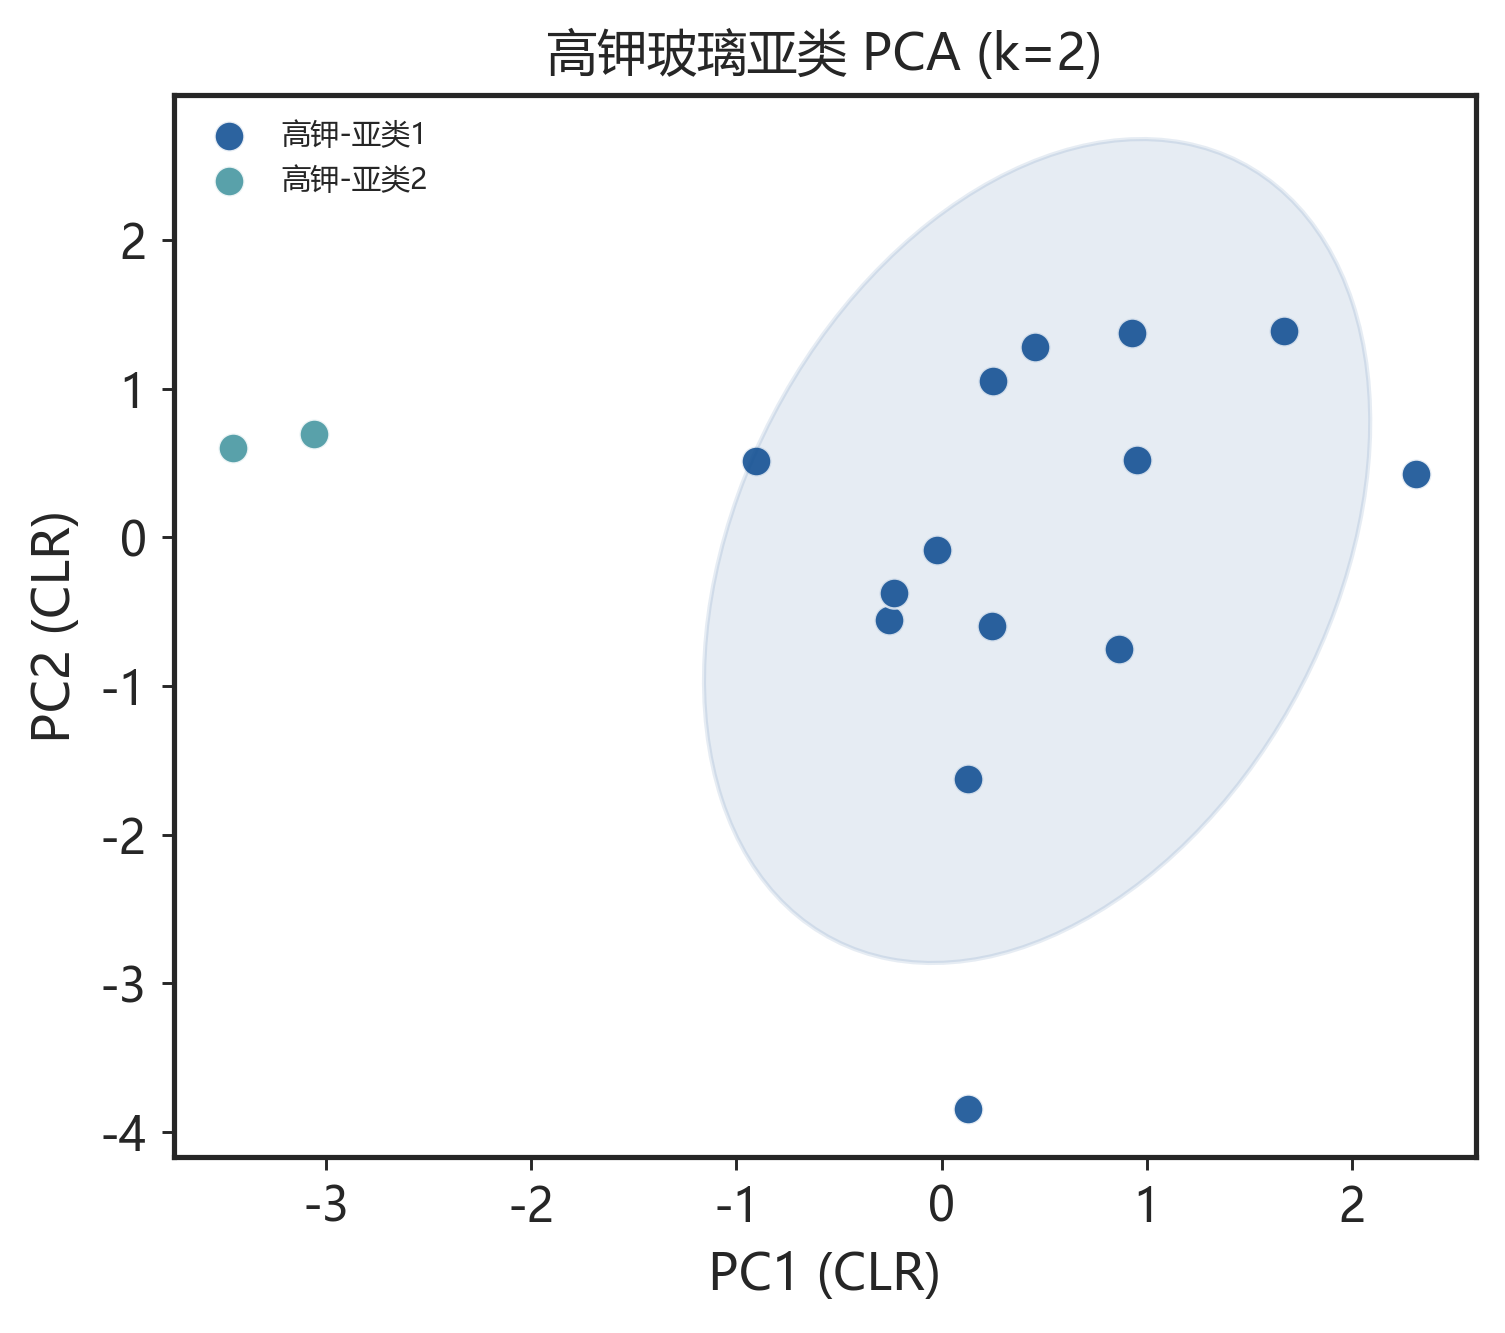
\includegraphics[width=\linewidth]{fig2_5_subclass_pca_高钾.png}
\caption{高钾亚类}
\end{subfigure}
\begin{subfigure}{0.48\textwidth}
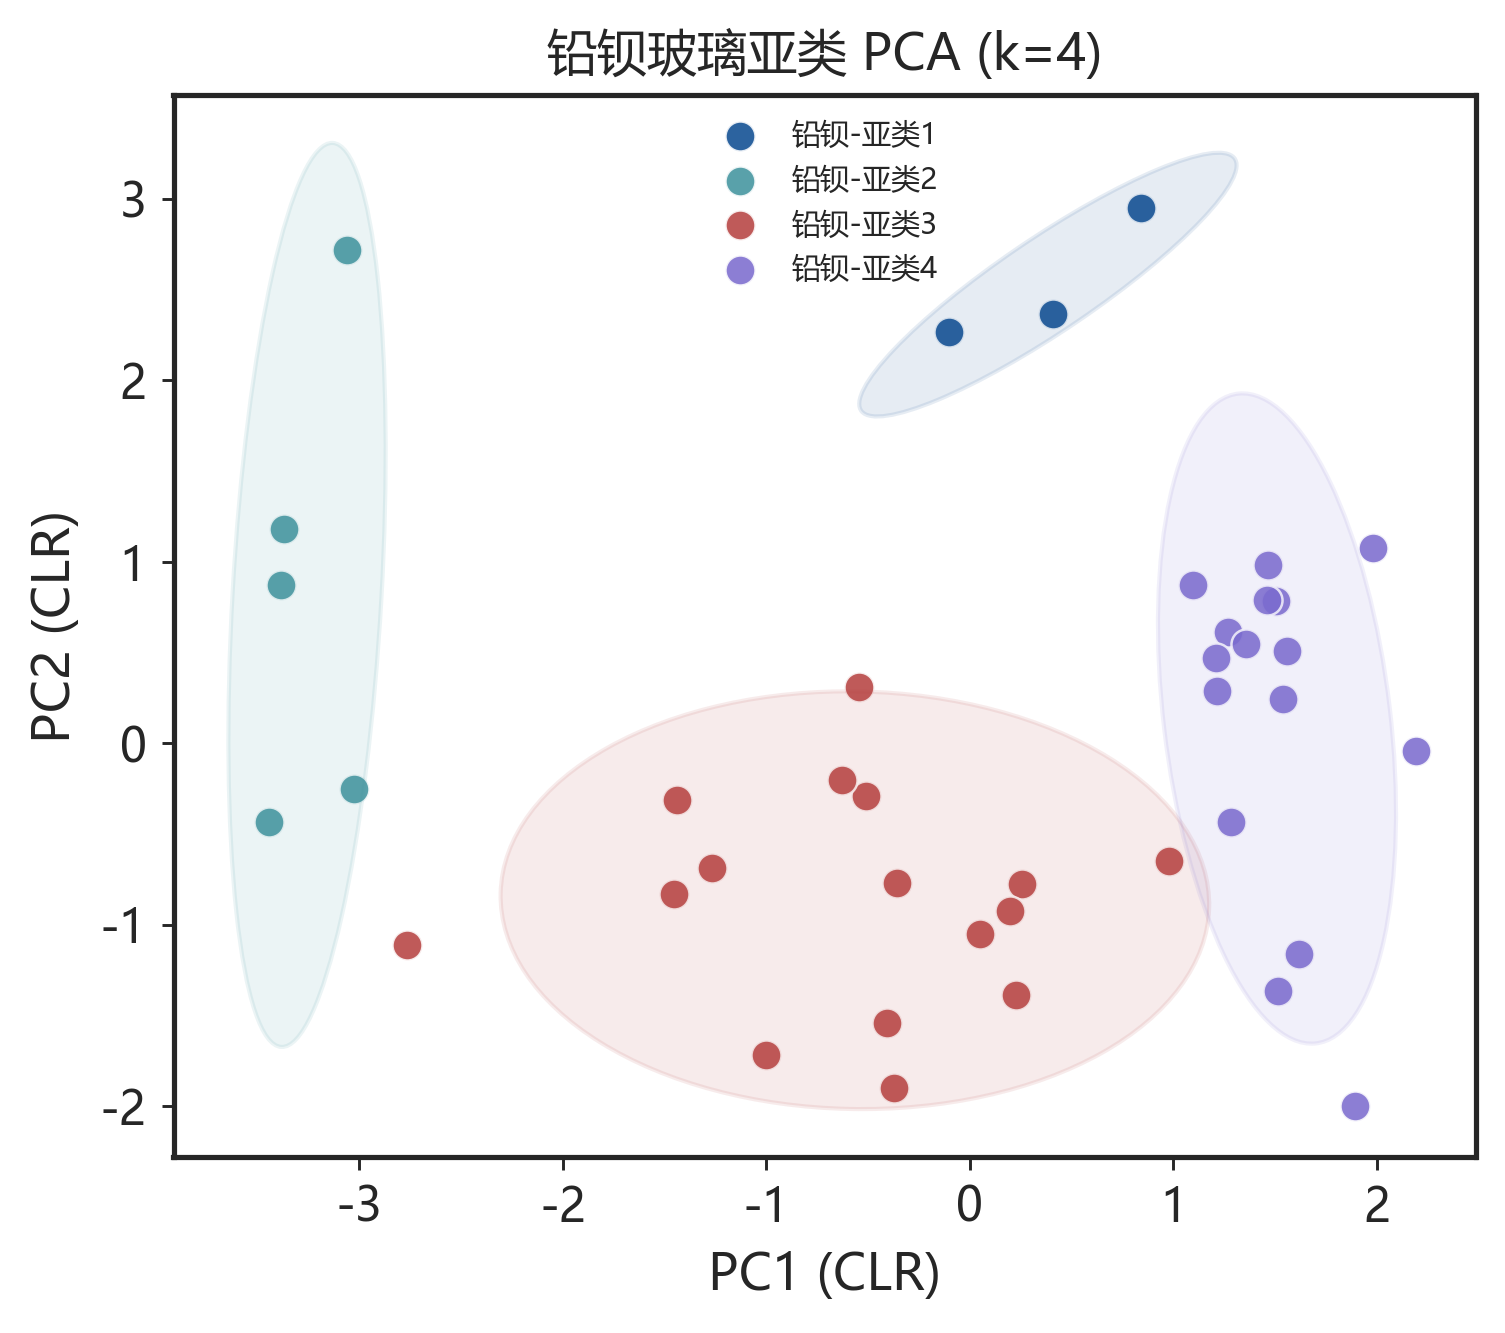
\includegraphics[width=\linewidth]{fig2_5_subclass_pca_铅钡.png}
\caption{铅钡亚类}
\end{subfigure}
\caption{亚类 PCA 可视化（含 $95\%$ 协方差椭圆）}
\label{fig:p2-pca}
\end{figure}

\begin{figure}[H]
\centering
\begin{subfigure}{0.48\textwidth}
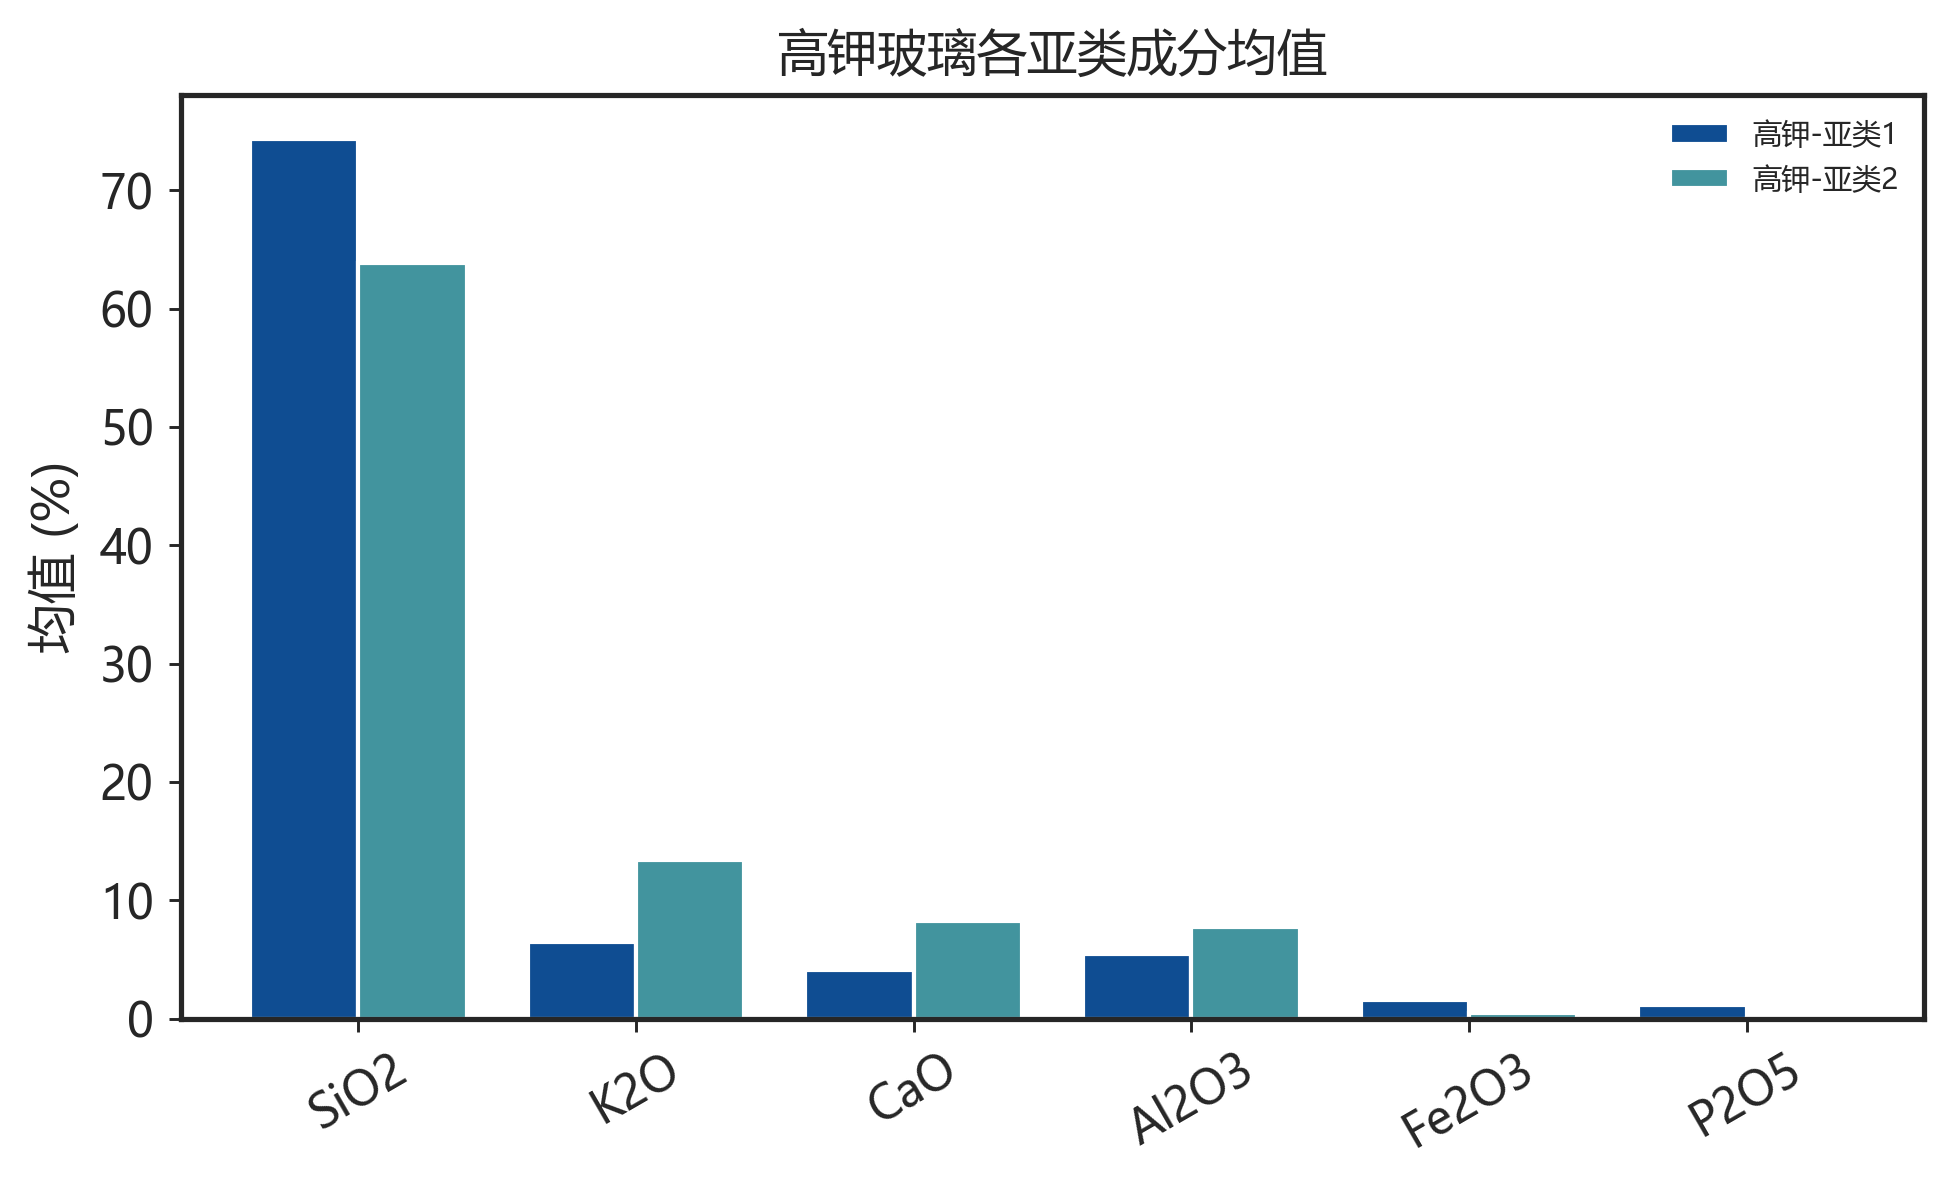
\includegraphics[width=\linewidth]{fig2_6_subclass_means_高钾.png}
\caption{高钾亚类均值}
\end{subfigure}
\begin{subfigure}{0.48\textwidth}
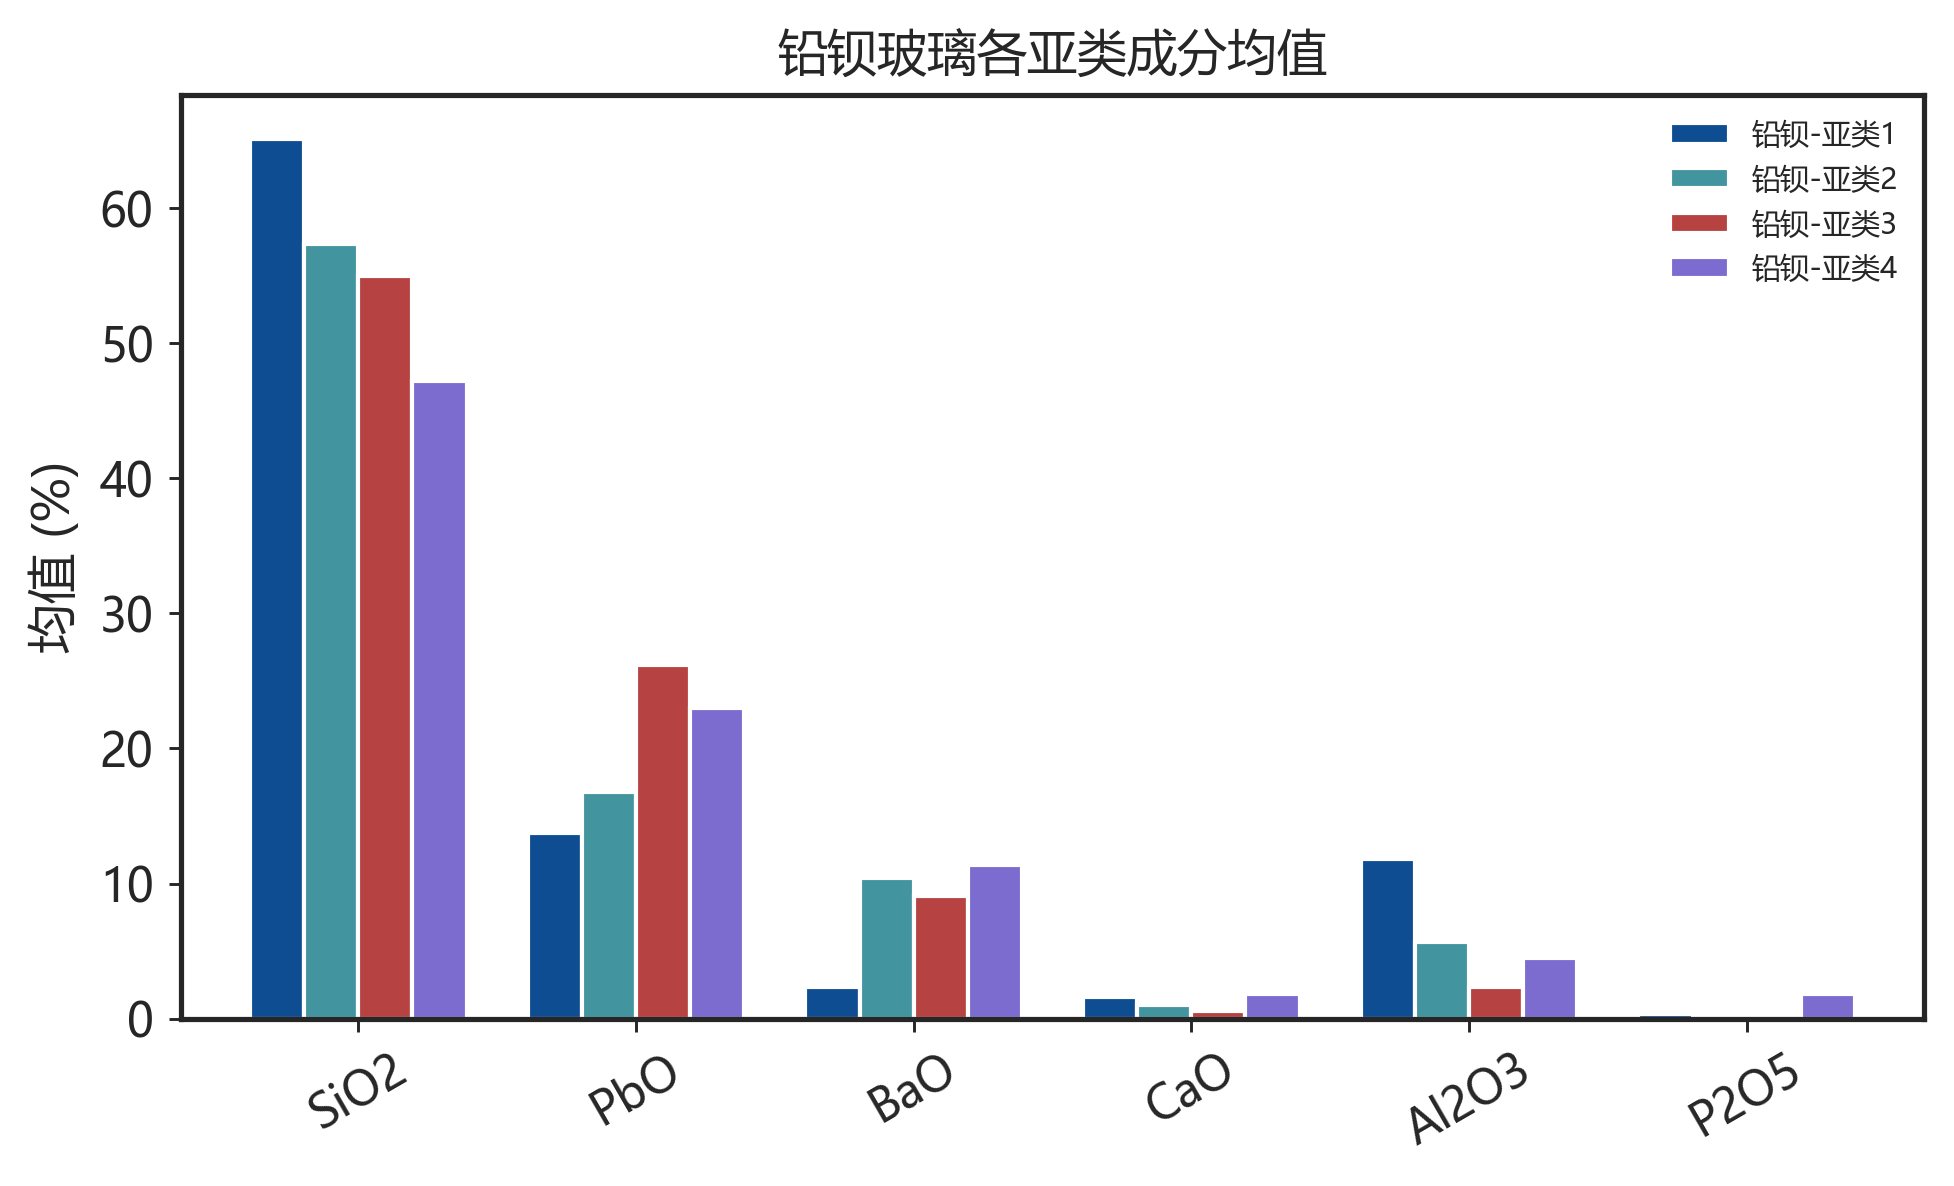
\includegraphics[width=\linewidth]{fig2_6_subclass_means_铅钡.png}
\caption{铅钡亚类均值}
\end{subfigure}
\caption{各亚类关键成分均值对比}
\label{fig:p2-means}
\end{figure}

\begin{table}[H]
\centering
\caption{亚类质心（主要成分，\%）与解释}
\label{tab:p2-center}
\footnotesize
\begin{tabular}{llccp{2.8cm}p{4.0cm}}
\toprule
类型 & 亚类 & $\mathrm{SiO_2}$ & $n$ & 关键特征 & 解释 \\
\midrule
高钾 & 亚类1 & 74.37 & 14 & K2O 6.48, CaO 4.12 & 高钾主组 \\
高钾 & 亚类2 & 63.83 & 2 & K2O 13.40, CaO 8.25 & 低硅富钾钙离群组 \\
铅钡 & 亚类1 & 65.16 & 3 & PbO 13.73, Al2O3 11.85 & 高硅高铝小样本组 \\
铅钡 & 亚类2 & 57.36 & 5 & PbO 16.80, BaO 10.44 & 中硅低铅小样本组 \\
铅钡 & 亚类3 & 54.95 & 16 & PbO 26.18, BaO 9.05 & 中硅中铅主组 \\
铅钡 & 亚类4 & 47.23 & 16 & PbO 22.98, BaO 11.40 & 低硅富钡磷主组 \\
\bottomrule
\end{tabular}
\end{table}

风化校正后，铅钡旧分群中“某簇几乎全为风化点”的现象明显减弱；高钾主组含 8 个无风化、6 个风化文物，小组仅含 2 个无风化文物。平均校正降低了风化分层，却不能把 $n=2$ 小组证实为真实工艺类别，因此只描述成分端元，不赋予产地语义。

\subsection{合理性与敏感性}

合理性用轮廓系数与校正后原空间方差削减比衡量。高钾方差削减比为 $0.486$、CLR 轮廓 $0.341$，但结果依赖仅 2 件的小组；铅钡方差削减比 $0.335$、轮廓 $0.321$，同样属于可讨论但不强的结构。

对成分施加相对高斯扰动 $x\leftarrow x(1+\varepsilon)$，$\varepsilon\sim\mathcal{N}(0,\sigma^2)$，计算与原划分的 ARI。结果应结合均值和标准差解释：低扰动下较稳定，但随 $\sigma$ 增大 ARI 下降且高钾波动明显，进一步说明小簇归属不应作确定结论。

\begin{figure}[H]
\centering
\begin{subfigure}{0.48\textwidth}
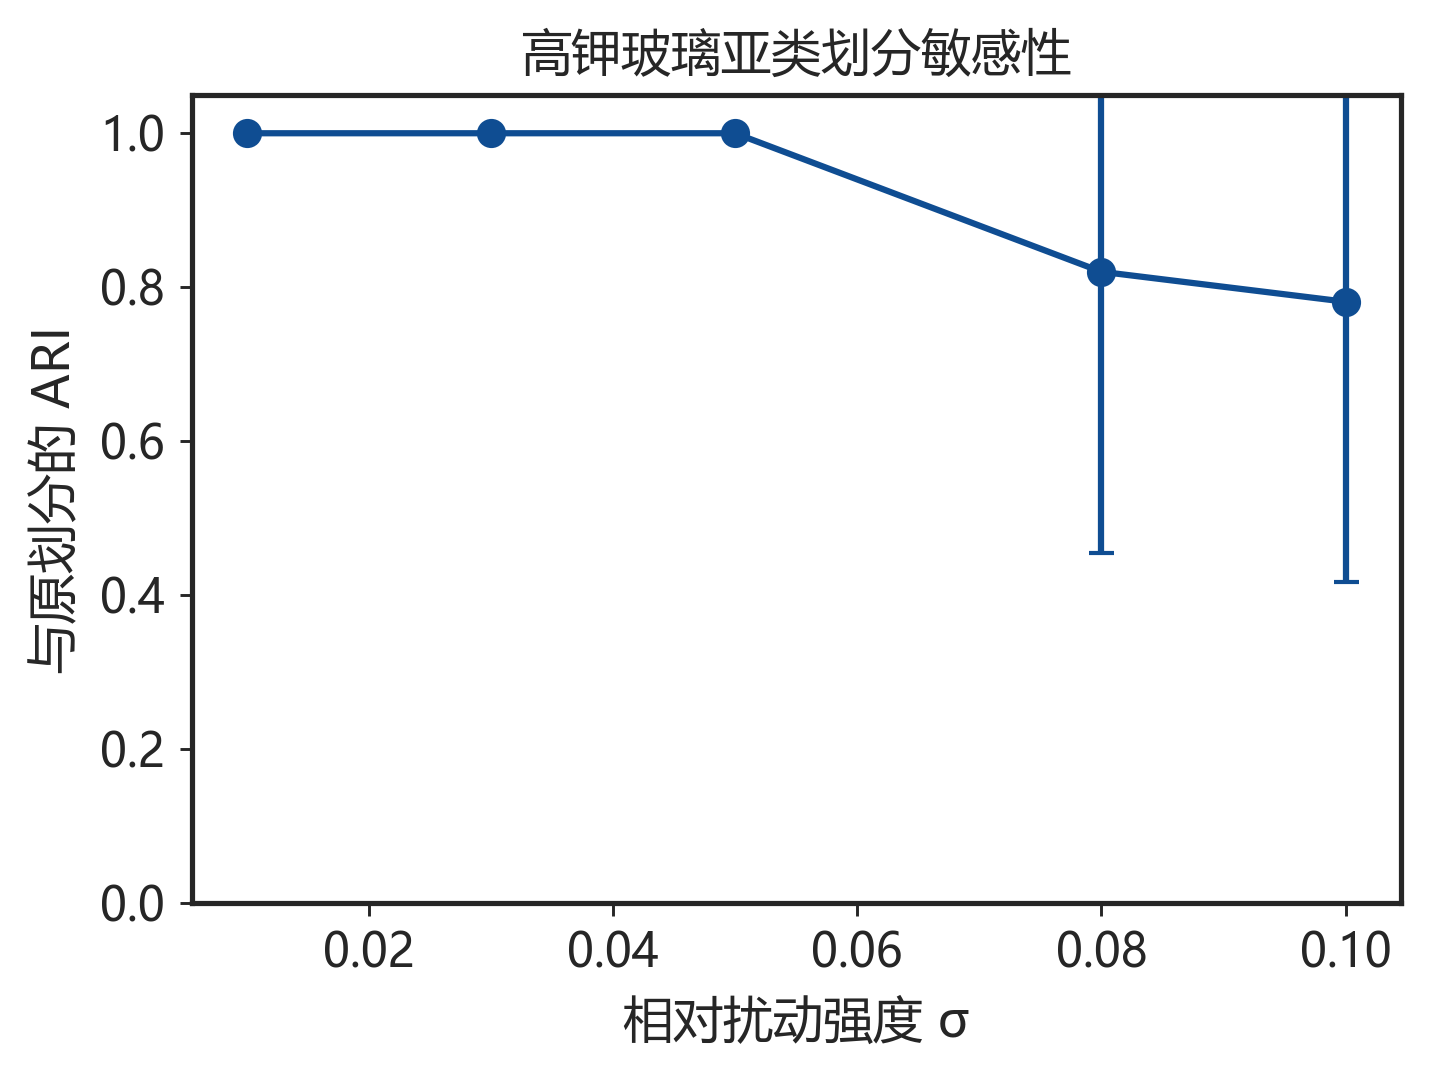
\includegraphics[width=\linewidth]{fig2_7_sensitivity_高钾.png}
\caption{高钾}
\end{subfigure}
\begin{subfigure}{0.48\textwidth}
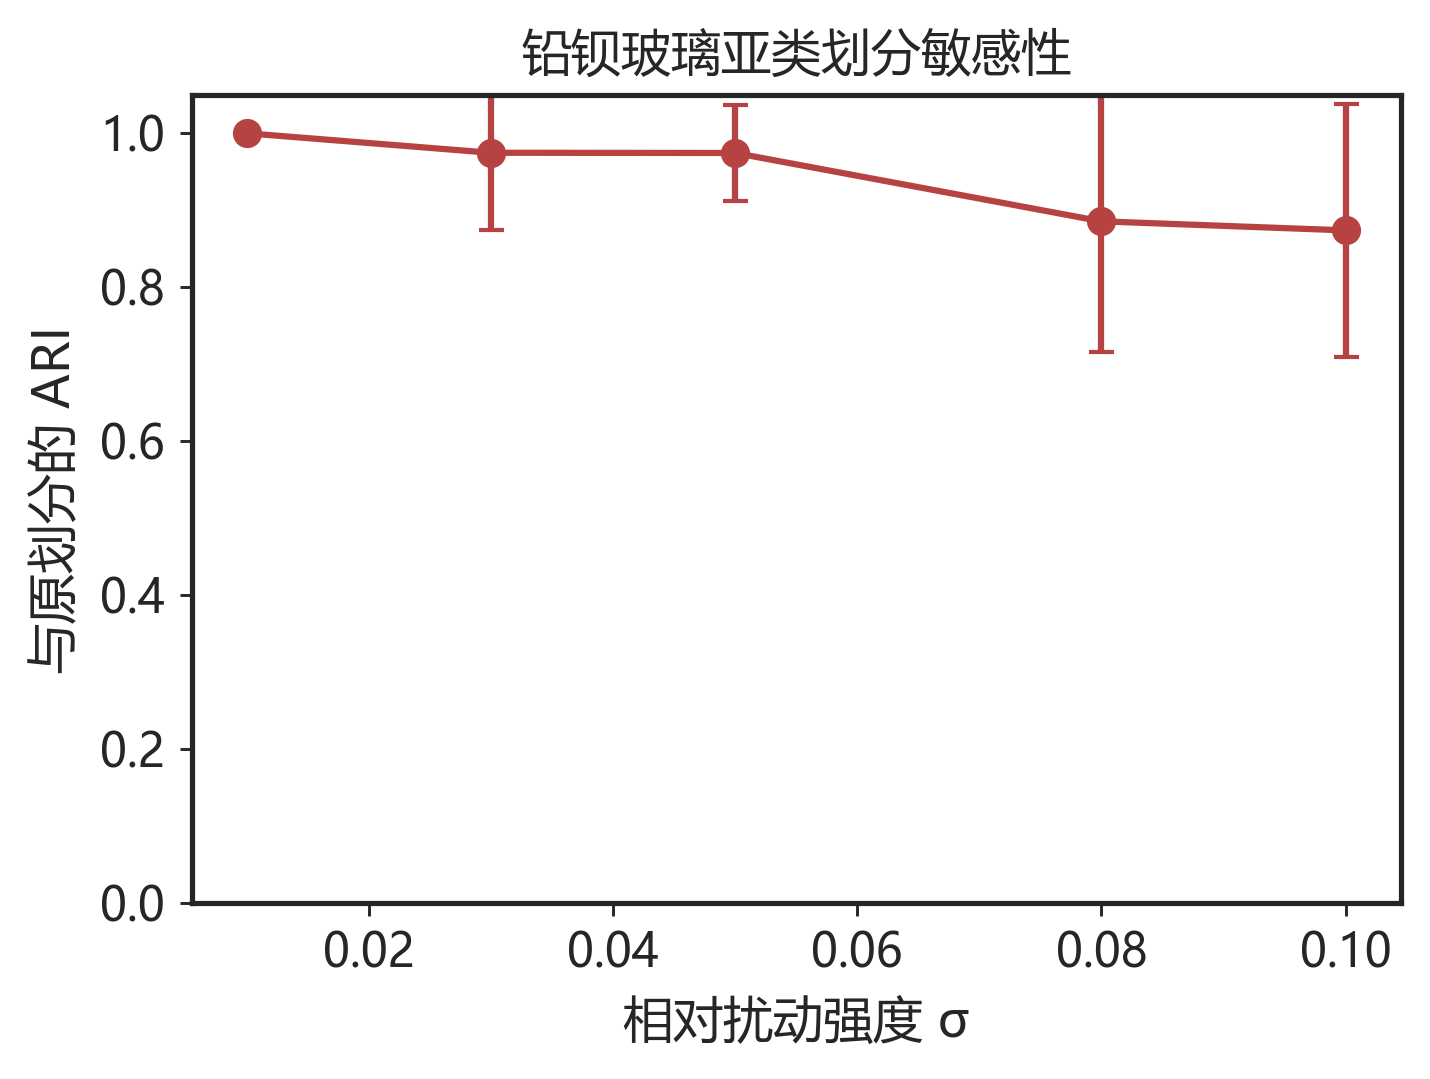
\includegraphics[width=\linewidth]{fig2_7_sensitivity_铅钡.png}
\caption{铅钡}
\end{subfigure}
\caption{亚类划分敏感性（ARI--$\sigma$）}
\label{fig:p2-sens}
\end{figure}

\begin{figure}[H]
\centering
\begin{subfigure}{0.48\textwidth}
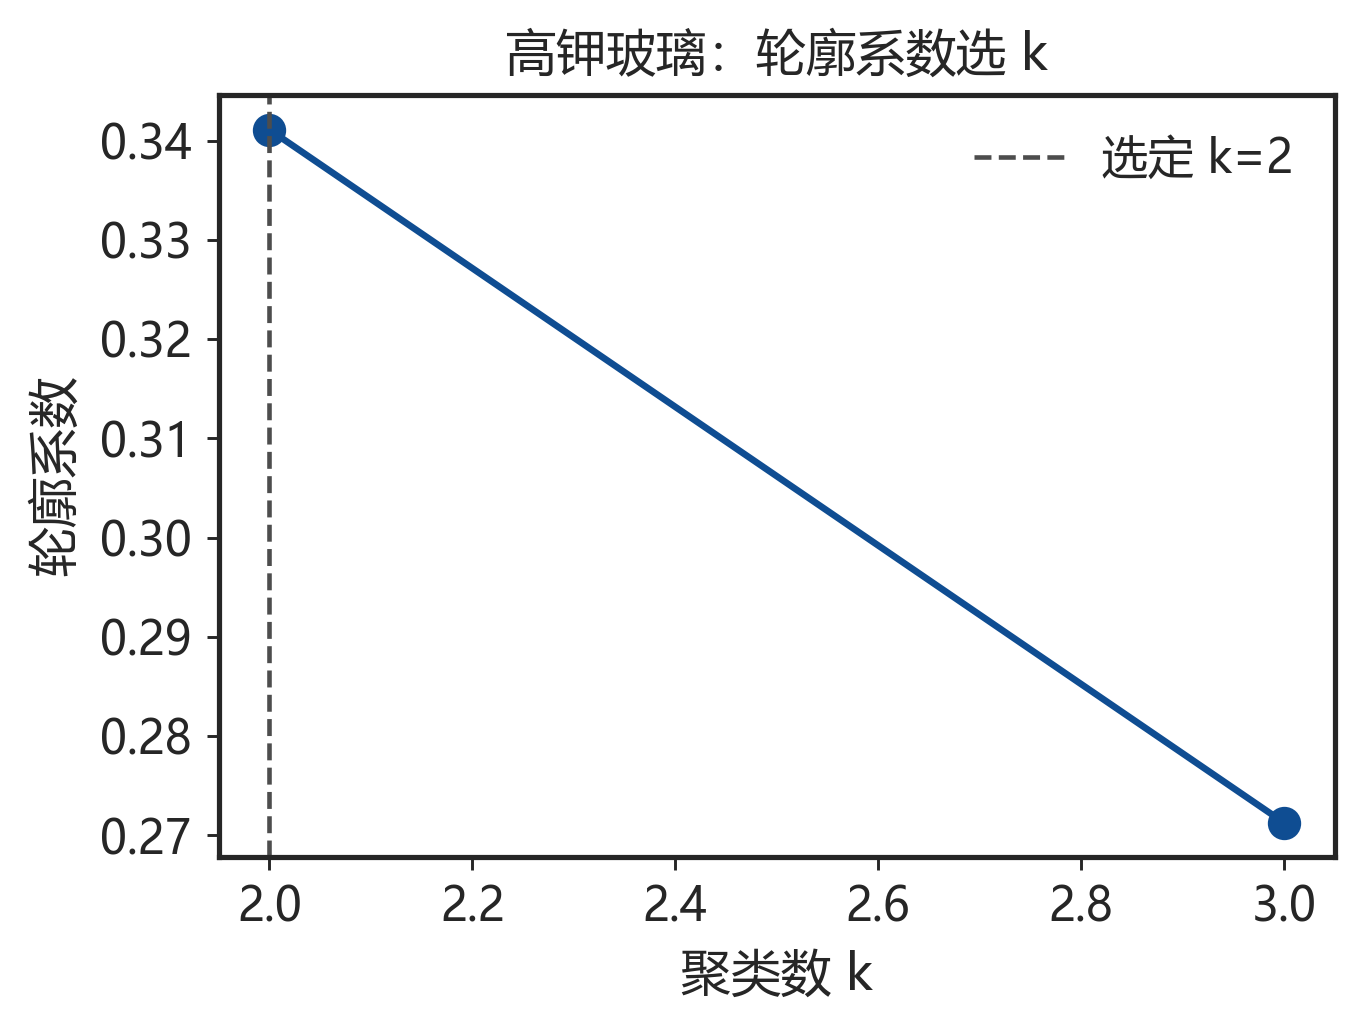
\includegraphics[width=\linewidth]{fig2_8_silhouette_高钾.png}
\caption{高钾}
\end{subfigure}
\begin{subfigure}{0.48\textwidth}
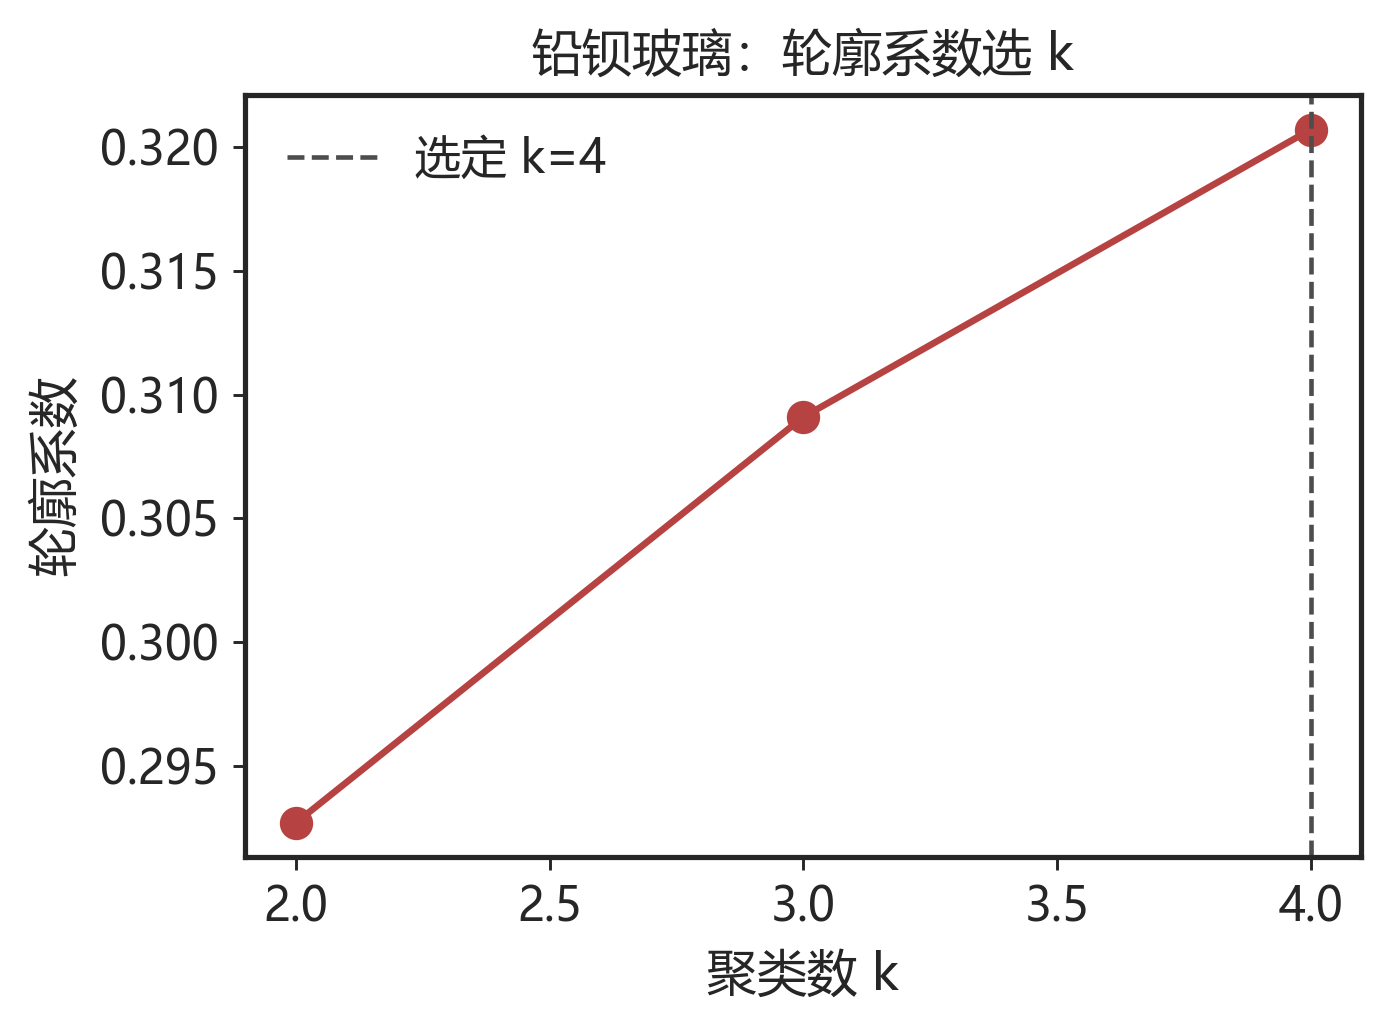
\includegraphics[width=\linewidth]{fig2_8_silhouette_铅钡.png}
\caption{铅钡}
\end{subfigure}
\caption{轮廓系数随 $k$ 变化（高钾 $k=2$，铅钡 $k=4$）}
\label{fig:p2-sil}
\end{figure}

% =========================================================
\section{问题三：未知样品鉴别}
% =========================================================

\subsection{鉴别模型}

在文物分组验证通过后，用全训练集拟合“随机森林+CLR--Logistic”集成，输出铅钡支持度
\[
s(\bm{x})=\frac{P_{\mathrm{RF}}(\text{铅钡}\mid\bm{x})
+P_{\mathrm{LR}}(\text{铅钡}\mid\mathrm{clr}(\bm{x}))}{2}.
\]
由于小样本下树投票和 Logistic 输出均未经过独立校准，本文不把 $s$ 称为“真实概率”。以 $s\ge0.5$ 判铅钡，并报告 200 次文物级 bootstrap 的 $95\%$ 区间和判别一致率。亚类归属先按预测类型校正风化位移，再在问题二同一 CLR 标准化空间取最近质心；这修复了“训练在 CLR 空间、预测却在原始百分比空间量距”的不一致。另用阈值规则及同类最近邻距离百分位交叉核验。

\begin{figure}[H]
\centering
\begin{subfigure}{0.48\textwidth}
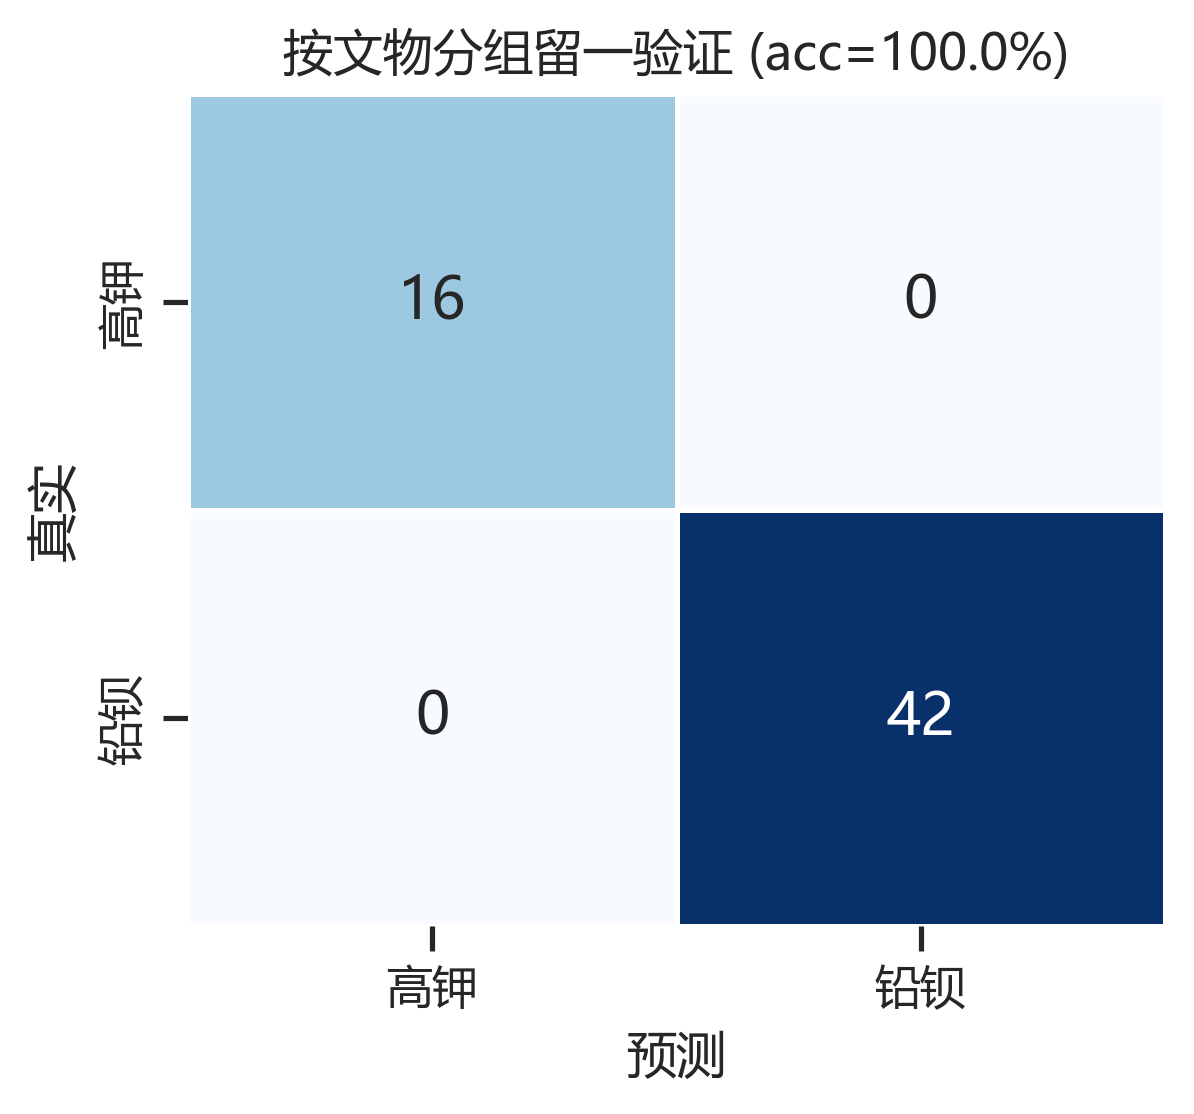
\includegraphics[width=\linewidth]{fig3_3_loo_cm.png}
\caption{按文物分组留一混淆矩阵}
\end{subfigure}
\begin{subfigure}{0.48\textwidth}
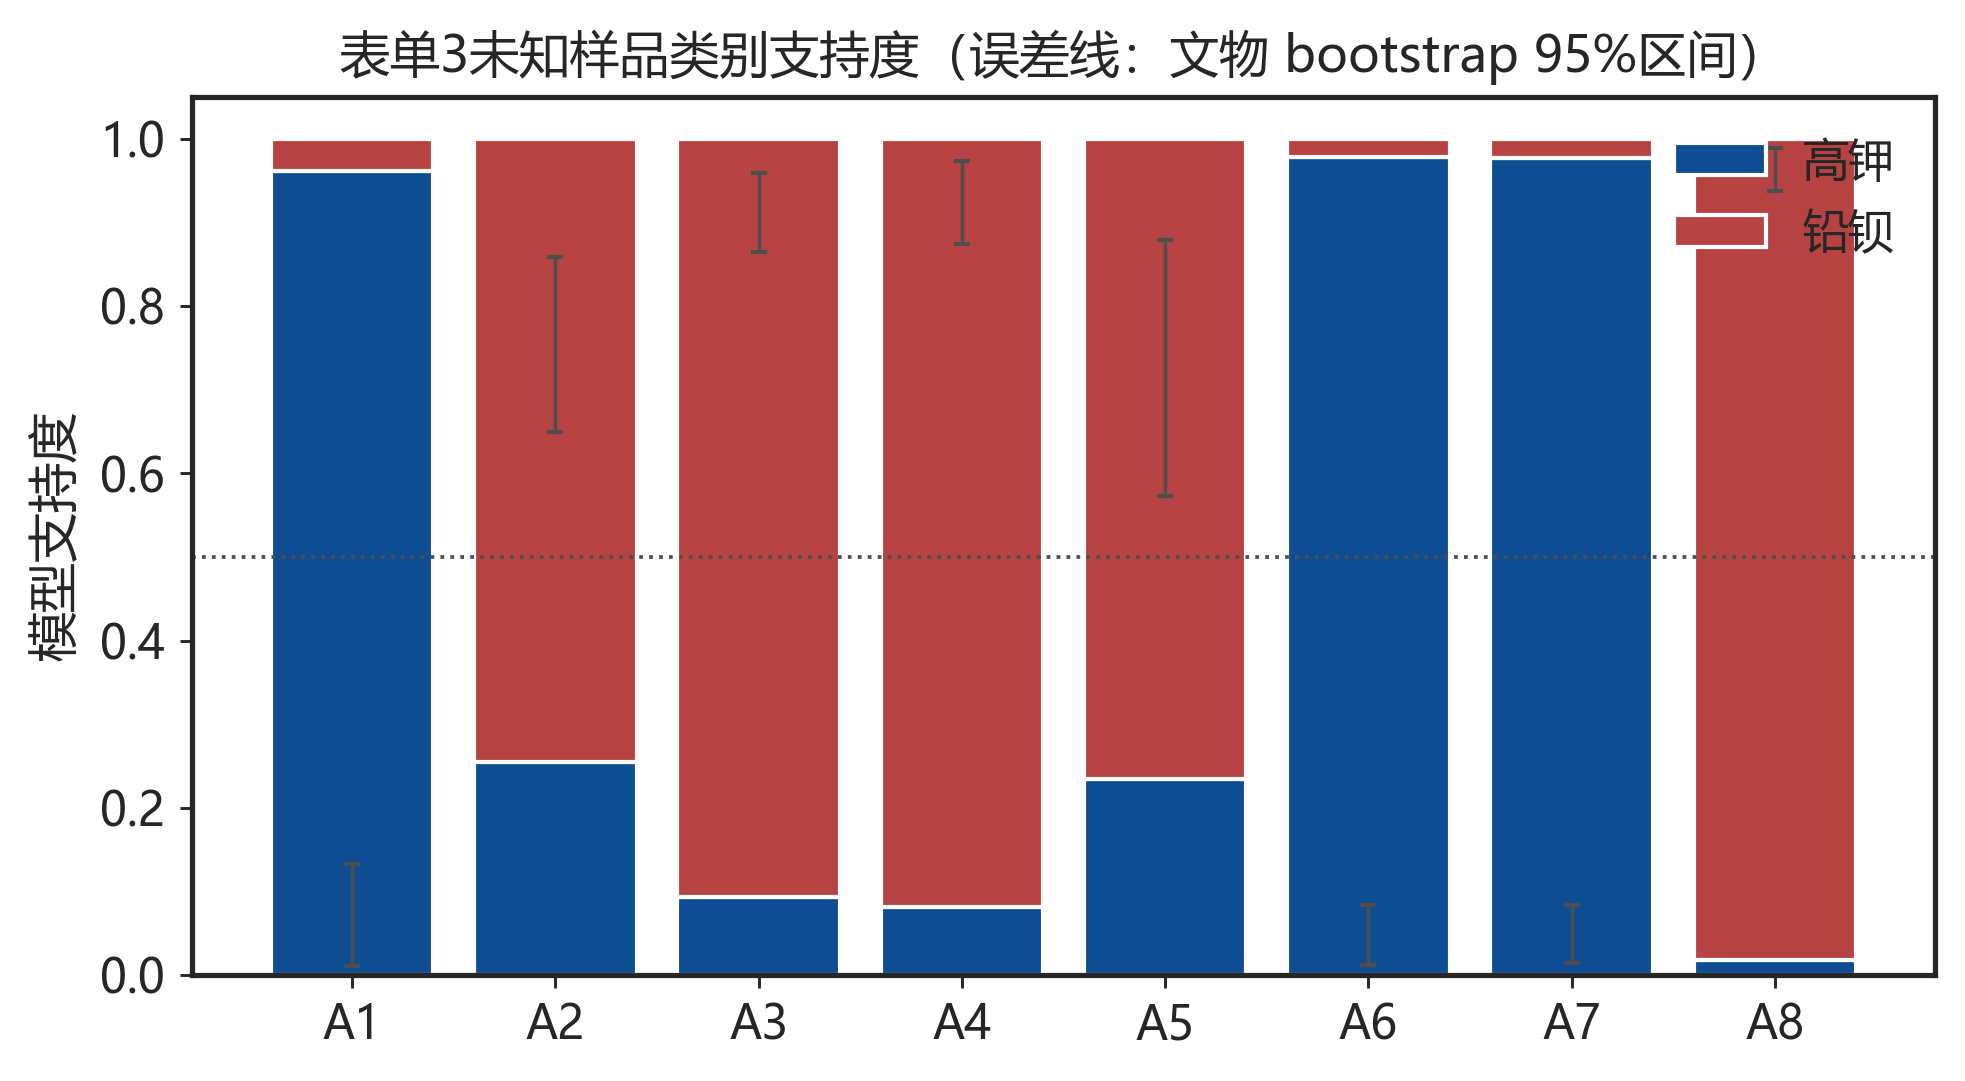
\includegraphics[width=\linewidth]{fig3_1_predict_proba.png}
\caption{未知样品模型支持度及 bootstrap 区间}
\end{subfigure}
\caption{分类器可靠性与表单3预测}
\label{fig:p3-main}
\end{figure}

\begin{table}[H]
\centering
\caption{表单3未知样品鉴别结果}
\label{tab:p3}
\begin{tabular}{ccccccc}
\toprule
编号 & 表面风化 & 预测类型 & 阈值规则 & 高钾支持度 & 铅钡支持度 & 预测亚类 \\
\midrule
A1 & 无风化 & \textbf{高钾} & 高钾 & 0.962 & 0.038 & 高钾-亚类1 \\
A2 & 风化 & \textbf{铅钡} & 铅钡 & 0.255 & 0.745 & 铅钡-亚类1 \\
A3 & 无风化 & \textbf{铅钡} & 铅钡 & 0.094 & 0.906 & 铅钡-亚类4 \\
A4 & 无风化 & \textbf{铅钡} & 铅钡 & 0.082 & 0.918 & 铅钡-亚类4 \\
A5 & 风化 & \textbf{铅钡} & 铅钡 & 0.234 & 0.766 & 铅钡-亚类1 \\
A6 & 风化 & \textbf{高钾} & 高钾 & 0.979 & 0.021 & 高钾-亚类1 \\
A7 & 风化 & \textbf{高钾} & 高钾 & 0.977 & 0.023 & 高钾-亚类2 \\
A8 & 无风化 & \textbf{铅钡} & 铅钡 & 0.018 & 0.982 & 铅钡-亚类4 \\
\bottomrule
\end{tabular}
\end{table}

\textbf{依据与交叉印证：}集成模型与阈值规则对 8 件样品完全一致，且 200 次文物 bootstrap 的类别一致率均为 1。A6、A7 的 $\mathrm{SiO_2}>90\%$ 且几乎无 $\mathrm{PbO/BaO}$，符合风化高钾特征；A2--A5、A8 的 $\mathrm{PbO}+\mathrm{BaO}$ 高于阈值；A1 无铅钡成分，判为高钾。A2 的适用域距离位于训练同类最近邻分布的 $97.6\%$ 分位，略超预设 $97.5\%$ 边界，因此其“铅钡”大类结论稳定，但细亚类和支持度应谨慎解释。

\subsection{敏感性分析}

对输入施加 $1\%\sim15\%$ 相对高斯扰动并统计翻转率；所有 8 件样品在各档扰动的 100 次重复中均未翻转。该结论只说明对设定的独立乘性检测误差稳定，不覆盖系统偏差、成分漏检机制改变或训练分布之外的新玻璃体系。

\begin{figure}[H]
\centering
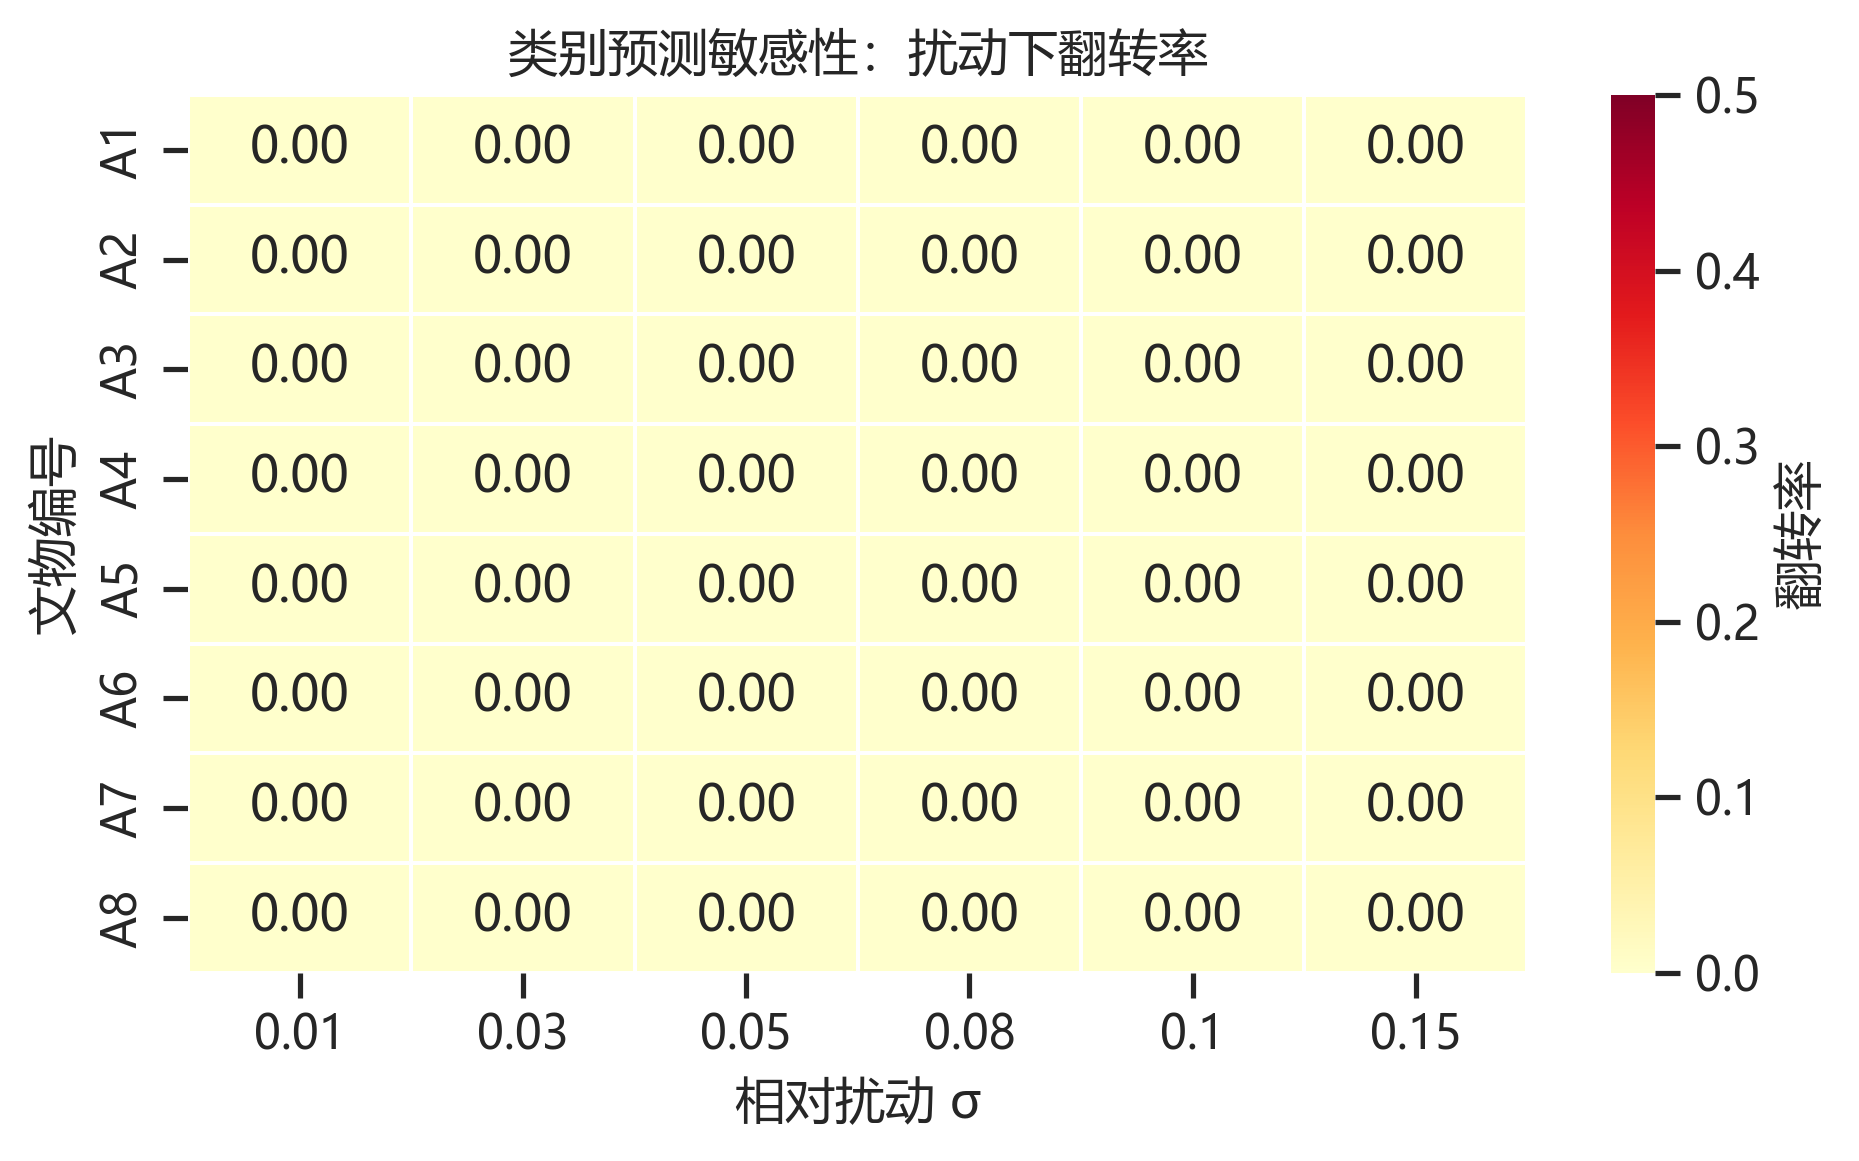
\includegraphics[width=0.75\textwidth]{fig3_2_sensitivity_flip.png}
\caption{未知样品类别预测翻转率热图}
\label{fig:p3-sens}
\end{figure}

% =========================================================
\section{问题四：成分关联及其类别差异}
% =========================================================

\subsection{组内关联模型}

先在采样点层面校正分类型平均风化位移，再将同一文物的多点取均值；文物级风化标签取表单1的「表面风化」，避免编号49、50的风化/未风化点被多数票混成采样标签后再做层内置换。仅保留两类中检出率均不低于 $20\%$ 且有足够变异的成分。对零值作成分自适应替换并闭合后，令 $l_j=\log x_j$；在每一类型内再按风化状态减去组均值，以控制残余风化差异。主关联指标采用比例协调系数
\[
\rho_{jk}=\frac{2\operatorname{cov}(l_j,l_k)}
{\operatorname{var}(l_j)+\operatorname{var}(l_k)},\qquad -1\le\rho_{jk}\le1.
\]
$\rho$ 接近 1 表示两成分近似按固定比例共同变化，接近 $-1$ 表示对数尺度反向变化。对每对成分在风化层内置换其中一列 499 次得到 $p$ 值并作 FDR 校正，另以 500 次文物 bootstrap 给出区间；原始 Spearman 只作为未处理定和约束和风化混杂的敏感性对照。

\begin{figure}[H]
\centering
\begin{subfigure}{0.48\textwidth}
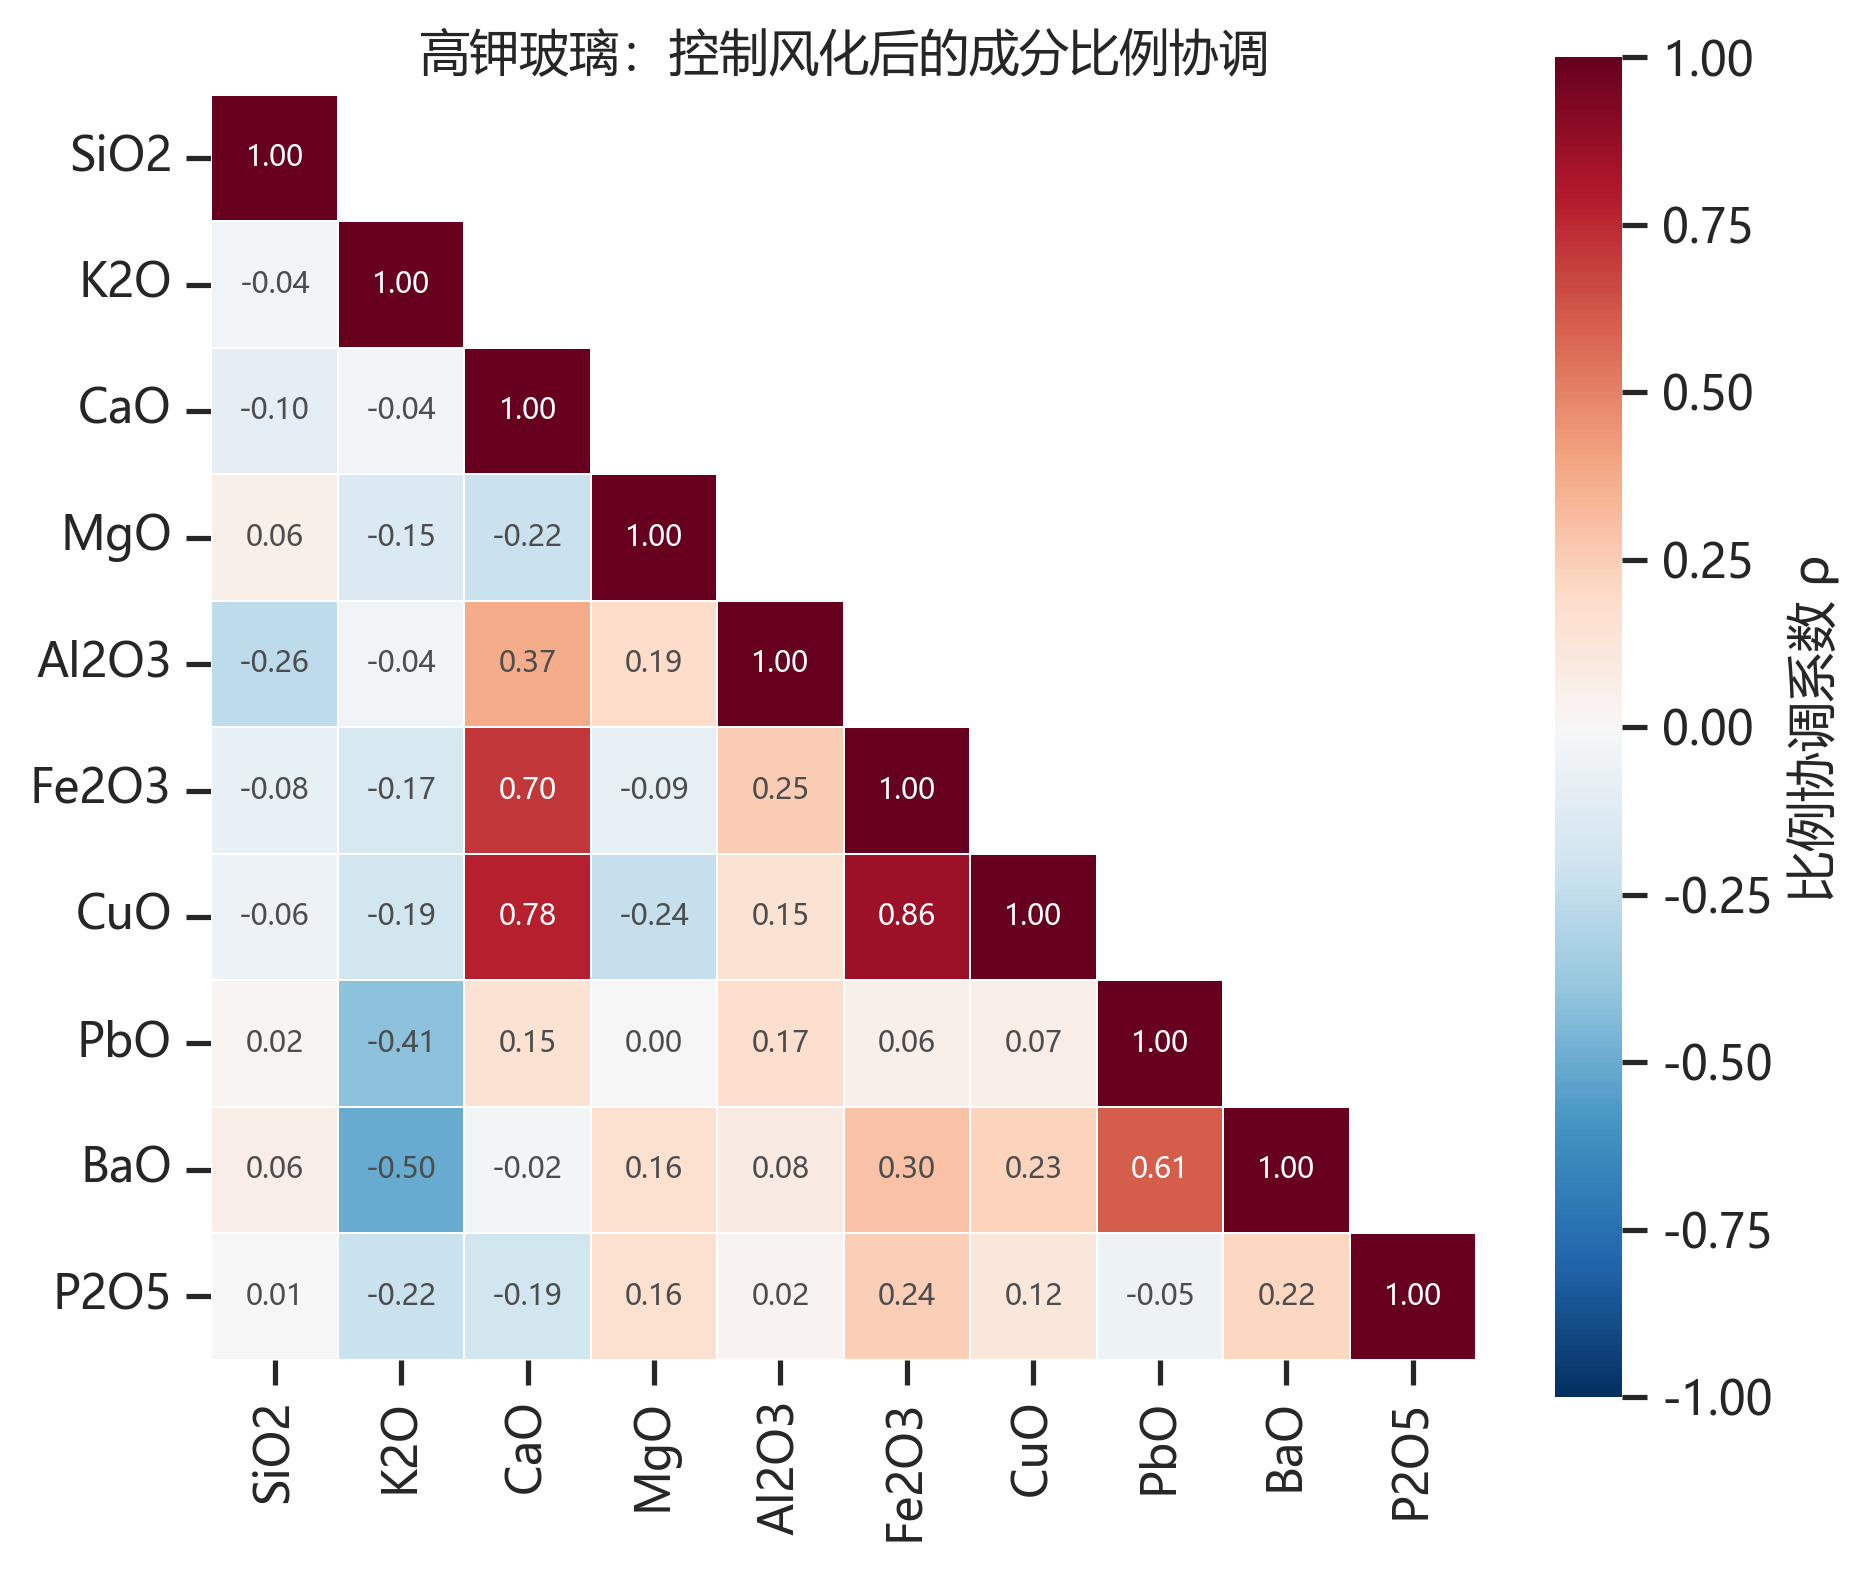
\includegraphics[width=\linewidth]{fig4_1_corr_高钾.png}
\caption{高钾比例协调}
\end{subfigure}
\begin{subfigure}{0.48\textwidth}
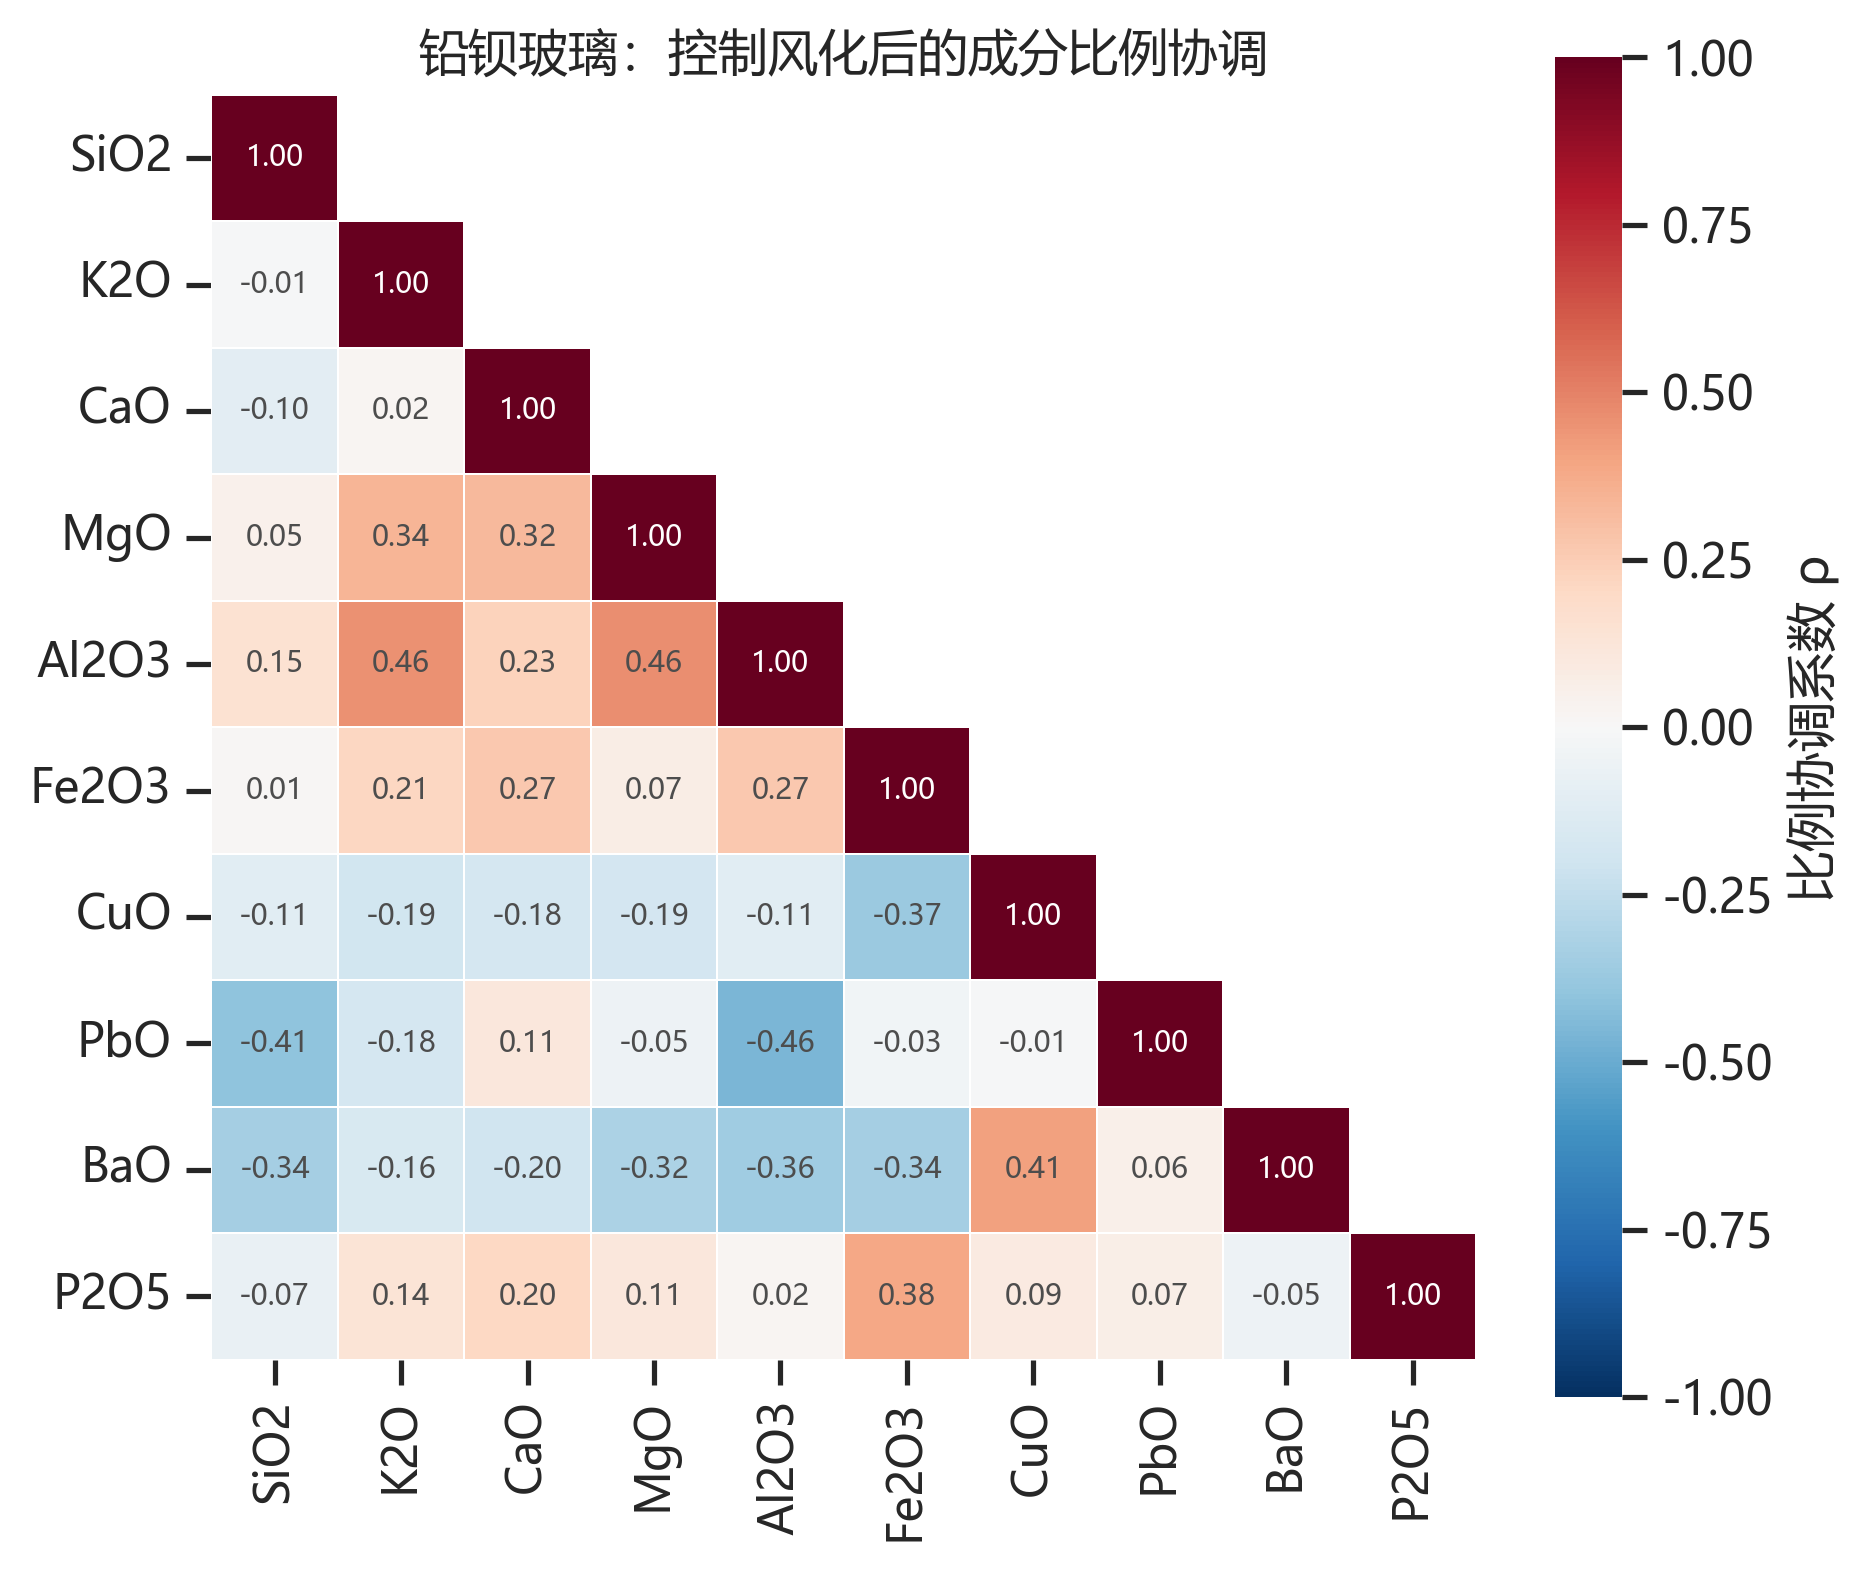
\includegraphics[width=\linewidth]{fig4_1_corr_铅钡.png}
\caption{铅钡比例协调}
\end{subfigure}
\caption{控制风化后的两类玻璃成分比例协调矩阵}
\label{fig:p4-corr}
\end{figure}

\begin{figure}[H]
\centering
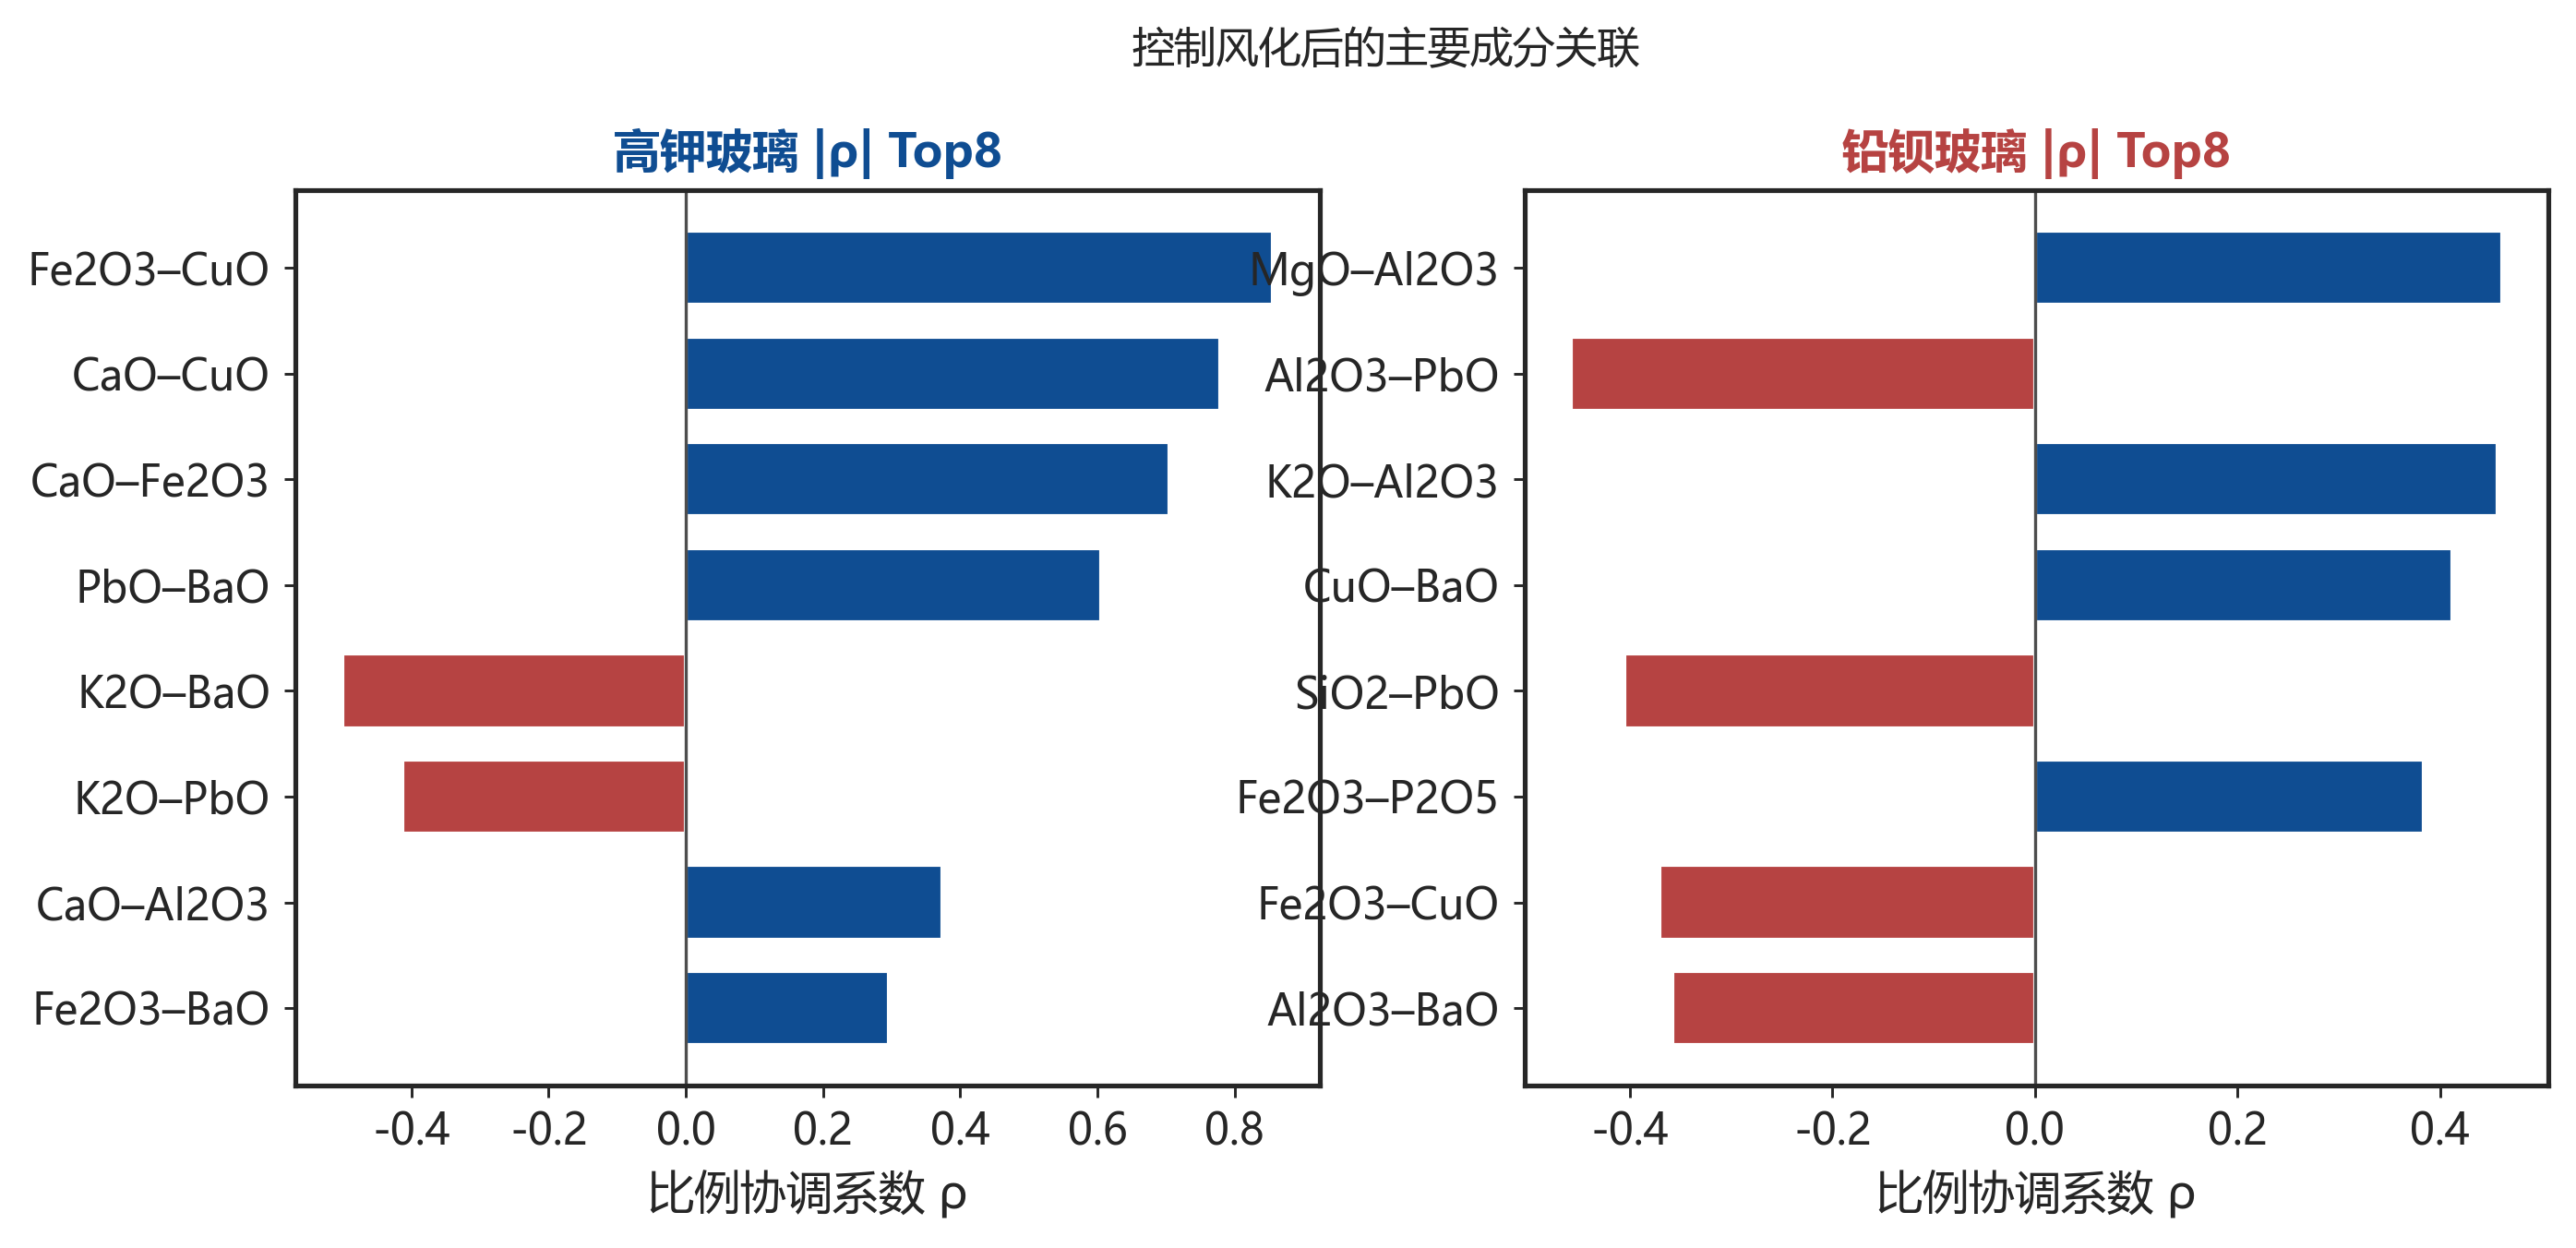
\includegraphics[width=0.85\textwidth]{fig4_4_top_pairs.png}
\caption{两类玻璃主要比例协调对（按 $|\rho|$ Top8）}
\label{fig:p4-top}
\end{figure}

\subsection{主要关联结论}
\begin{itemize}[leftmargin=2em]
  \item \textbf{高钾：}最强比例协调为 $\mathrm{Fe_2O_3}$--$\mathrm{CuO}$（$\rho=0.856$，bootstrap 95\% CI $[0.271,0.944]$）；但组内成对置换经 FDR 后 $q=0.072$，故只视为候选协同，不能写成已确认机制。FDR 显著的组内关联为 $\mathrm{K_2O}$--$\mathrm{BaO}$（$\rho=-0.501$）与 $\mathrm{SiO_2}$--$\mathrm{Al_2O_3}$（$\rho=-0.262$）。
  \item \textbf{铅钡：}$\mathrm{MgO}$--$\mathrm{Al_2O_3}$ 呈稳健正向协调（$\rho=0.461$，CI $[0.190,0.700]$）；$\mathrm{Al_2O_3}$--$\mathrm{PbO}$ 呈反向协调（$\rho=-0.458$，CI $[-0.624,-0.168]$）；$\mathrm{SiO_2}$--$\mathrm{PbO}$ 亦呈反向协调（$\rho=-0.405$，CI $[-0.616,-0.189]$），组内 FDR 分别为 $0.0225$、$0.0225$、$0.045$。
  \item \textbf{敏感性对照：}原始 Spearman 中若干“高硅--低助熔”强负相关在比例协调分析中明显减弱，说明旧结论主要混合了定和约束与风化组间差异；化学解释应以控制风化后的 $\rho$ 为主。
\end{itemize}

\subsection{类别间差异性}

旧流程把相关矩阵上三角元素任意打乱，既未保持矩阵对称/半正定结构，也不对应 Mantel 的行列同步置换，因此原 $p=0.161$ 无效。本文直接检验
\[
T=\left\|\operatorname{upper}\!\left(
R_{\rho}^{\text{高钾}}-R_{\rho}^{\text{铅钡}}\right)\right\|_2.
\]
在每个风化层内整体置换“类型”标签，保持类型$\times$风化样本构成；每次重新残差化并计算两张完整矩阵。观察到 $T=2.535$，999 次分层置换得 $p=0.002$，支持两类总体关联结构存在差异。逐对差异再作 FDR，确认 8 对：$\mathrm{SiO_2}$--$\mathrm{PbO}$、$\mathrm{SiO_2}$--$\mathrm{BaO}$、$\mathrm{K_2O}$--$\mathrm{Al_2O_3}$、$\mathrm{Al_2O_3}$--$\mathrm{PbO}$、$\mathrm{PbO}$--$\mathrm{BaO}$、$\mathrm{Fe_2O_3}$--$\mathrm{CuO}$、$\mathrm{CaO}$--$\mathrm{CuO}$（均 $q=0.0064$）以及 $\mathrm{Al_2O_3}$--$\mathrm{BaO}$（$q=0.017$）。

\begin{figure}[H]
\centering
\begin{subfigure}{0.48\textwidth}
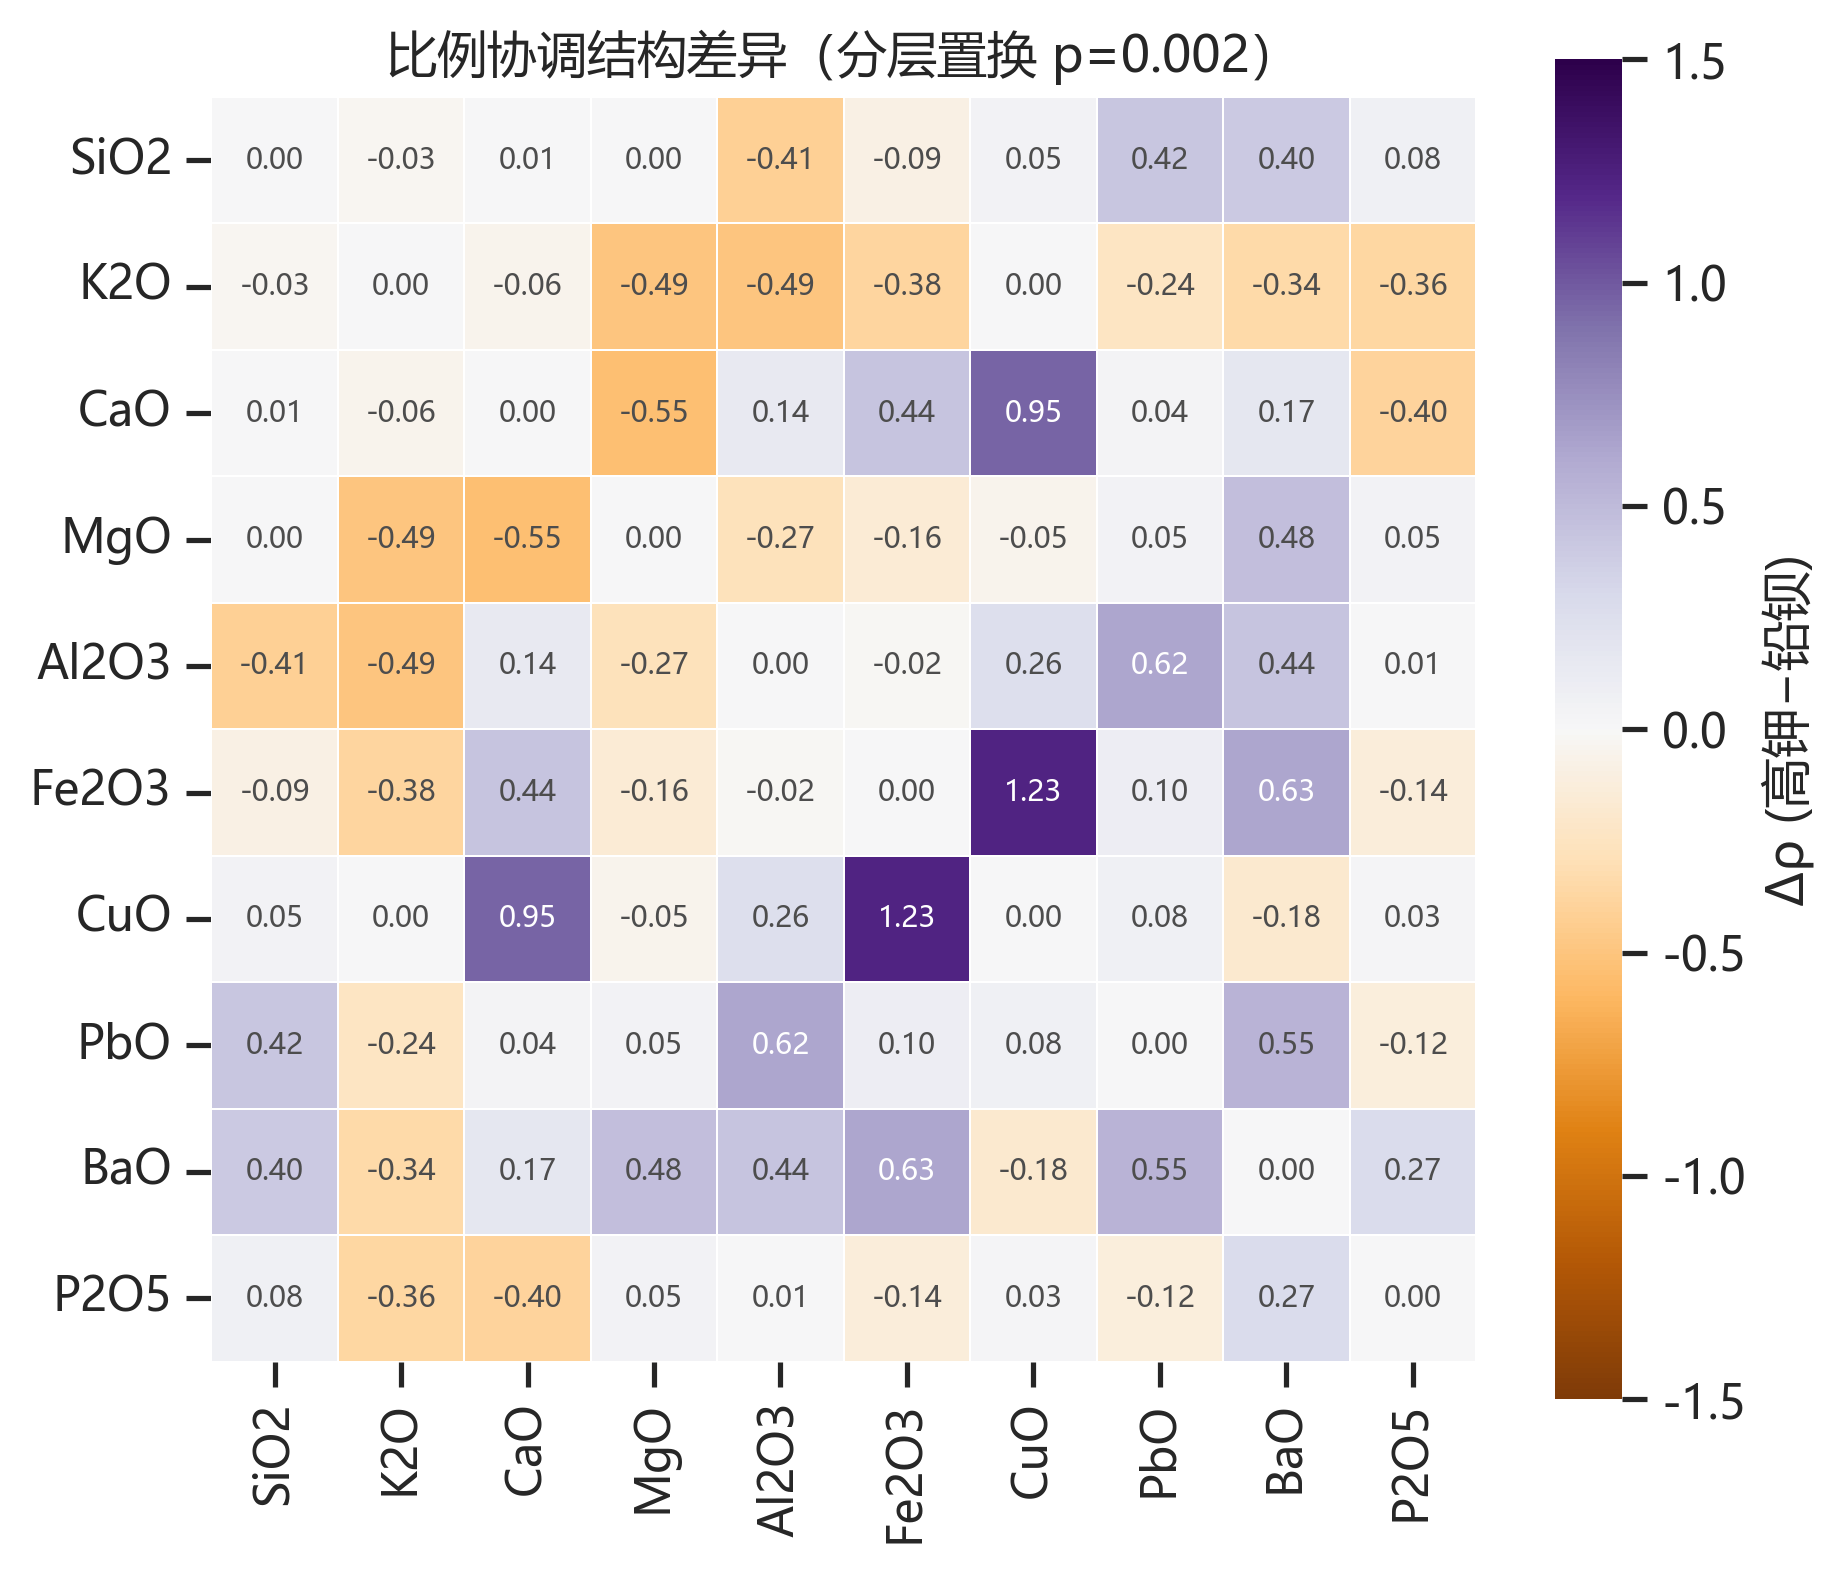
\includegraphics[width=\linewidth]{fig4_3_corr_diff.png}
\caption{比例协调差矩阵}
\end{subfigure}
\begin{subfigure}{0.48\textwidth}
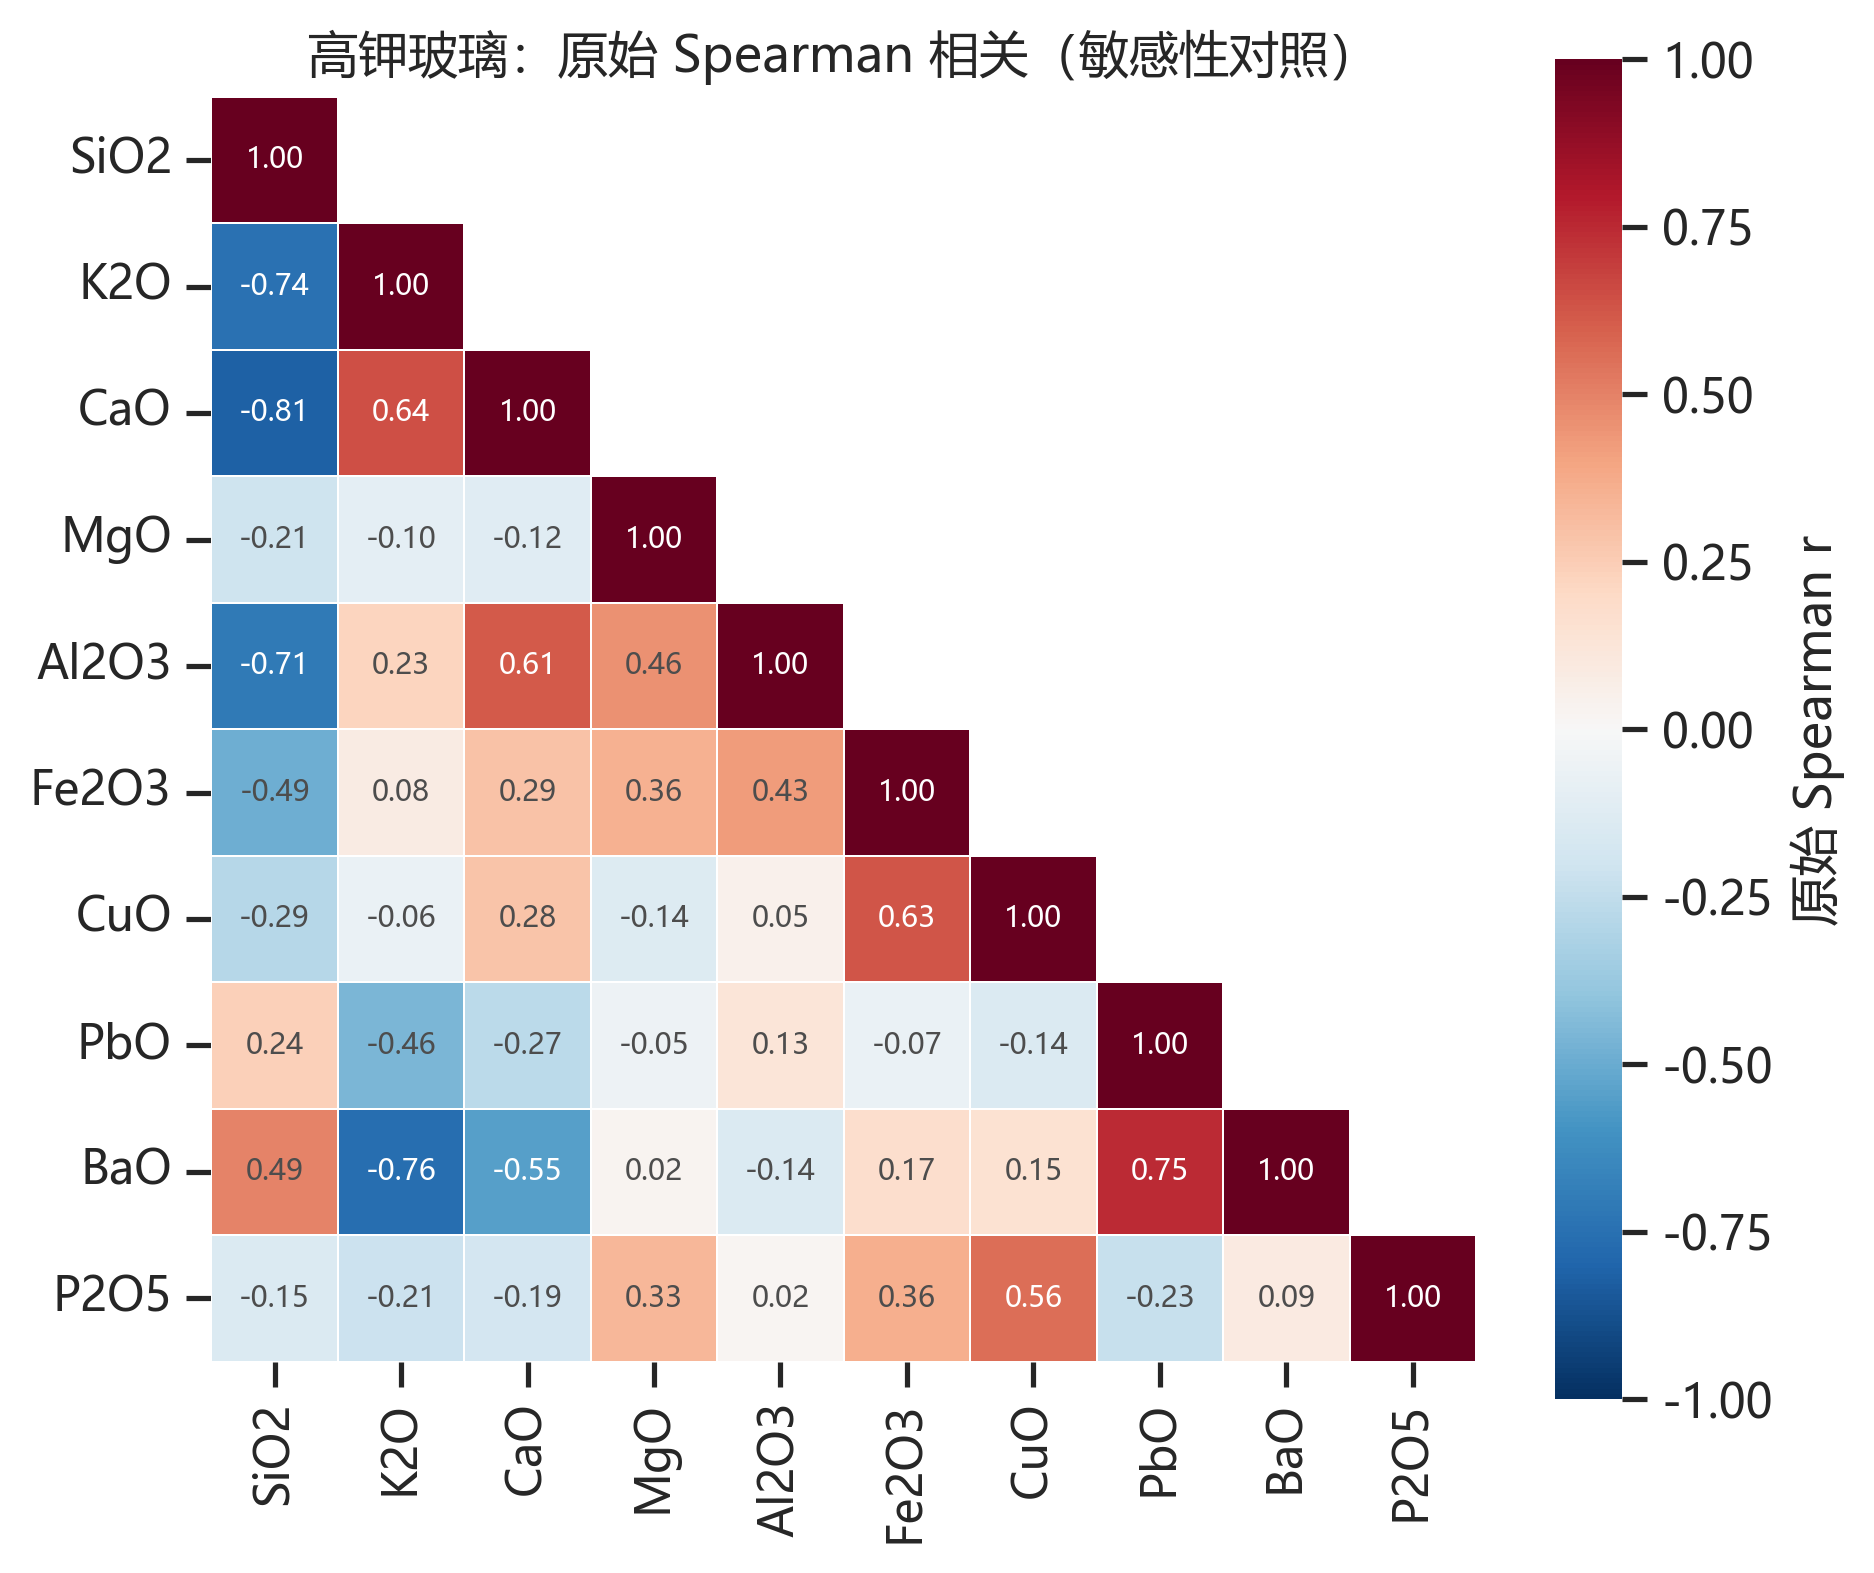
\includegraphics[width=\linewidth]{fig4_2_clr_corr_高钾.png}
\caption{高钾原始 Spearman（对照）}
\end{subfigure}
\caption{类别关联差异与原始相关敏感性对照}
\label{fig:p4-diff}
\end{figure}

% =========================================================
\section{模型评价与推广}
% =========================================================

\subsection{优点}
\begin{enumerate}[leftmargin=2em]
  \item 明确区分采样点与文物：推断使用文物级单元，验证按文物分组，消除了伪重复和跨折泄漏；
  \item 风化还原、亚类距离和未知归属统一在 CLR 几何中完成，训练与预测空间一致；
  \item 问题三同时报告 bootstrap、扰动和适用域；问题四使用保持实验结构的分层置换，结论均可复核。
\end{enumerate}

\subsection{不足与改进}
\begin{enumerate}[leftmargin=2em]
  \item 风化前预测仍是类型平均位移，缺少同一位置风化前后的真值；收缩只能降低方差，不能消除埋藏环境偏差；
  \item 高钾文物数较少，亚类轮廓系数不高，亚类只能称为数据驱动候选组，不能直接解释为产地或工艺流派；
  \item 模型支持度未在独立外部样本上校准；A2 略超训练适用域，需优先增加相似样本或人工复核；
  \item 零值替换依赖“最小正检出值的一半”这一近似；若获得实验室检测限，应改用真实检测限及其不确定性。
\end{enumerate}

\subsection{推广}
方法可迁移至陶瓷、青铜锈蚀产物等成分型文物分析：先做定和检验与风化校正，再用 CLR+聚类发现工艺亚型，最后以可解释分类器辅助考古鉴别。

% =========================================================
\section{结论}
% =========================================================

\begin{enumerate}[leftmargin=2em]
  \item Fisher/置换检验确认表面风化与玻璃类型相关（$p=0.0113$），纹饰和颜色证据不足；分类型风化方向不同，CLR 收缩位移给出了满足成分性的平均还原。
  \item $\mathrm{PbO}$ 与 $\mathrm{BaO}$ 是大类鉴别的核心指标；严格按文物分组并嵌套寻阈值后，阈值和集成模型在内部验证中均完全区分两类，但不把内部 $100\%$ 外推为普遍准确率。
  \item 表单3中 A1、A6、A7 为高钾，A2、A3、A4、A5、A8 为铅钡；bootstrap 与扰动结论稳定，A2 因适用域距离偏高需谨慎。
  \item 控制风化后的比例协调结构在两类间存在总体差异（分层置换 $p=0.002$），FDR 确认 8 个差异成分对。
\end{enumerate}

% =========================================================
\clearpage
\phantomsection
\addcontentsline{toc}{section}{参考文献}
\begin{center}{\fontsize{15pt}{20pt}\heiti 参考文献}\end{center}
\vspace{0.6em}
\begin{thebibliography}{99}
\setlength{\itemsep}{0.35em}
\bibitem{aitchison1986}
J.~Aitchison.
\newblock \emph{The Statistical Analysis of Compositional Data}.
\newblock Chapman \& Hall, 1986.

\bibitem{breiman2001}
L.~Breiman.
\newblock Random forests.
\newblock \emph{Machine Learning}, 45(5):5--32, 2001.

\bibitem{bh1995}
Y.~Benjamini and Y.~Hochberg.
\newblock Controlling the false discovery rate: a practical and powerful approach to multiple testing.
\newblock \emph{Journal of the Royal Statistical Society: Series B}, 57(1):289--300, 1995.

\bibitem{cumcm2022c}
全国大学生数学建模竞赛组委会.
\newblock 2022 高教社杯全国大学生数学建模竞赛题目 C 题.
\newblock 2022.

\bibitem{lovell2015}
D.~Lovell, V.~Pawlowsky-Glahn, J.~J. Egozcue, S.~Marguerat, and J.~Bähler.
\newblock Proportionality: A valid alternative to correlation for relative data.
\newblock \emph{PLoS Computational Biology}, 11(3):e1004075, 2015.
\end{thebibliography}

\clearpage
\phantomsection
\addcontentsline{toc}{section}{附录\quad 支撑材料清单}
\begin{center}{\fontsize{15pt}{20pt}\heiti 附录\quad 支撑材料清单}\end{center}
\vspace{0.6em}
\begin{itemize}
  \item 代码：\texttt{code/solve\_all.py}
  \item 结果表：\texttt{results/*.csv, *.json}
  \item 图件：\texttt{figures/*.png}（含方法对照图 \texttt{fig2\_9\_method\_compare.png}）
\end{itemize}

\end{document}
